\chapter{IGA based optimisation scheme}
%The way to build the optimization chain with metamodelisation Paper2

\subsection{IGA optimization setting}

In this section, we detail the shape optimization defined through NURBS parameterization of shapes for the pad, with its associated constraints and objectives for optimization. We also provide a short description of parameterization and refinement strategy for the disc-pad system domain $\Omega^{(\mathrm{d-p})}$.\\

The optimization is defined for the boundary $\partial \Gamma_{C}^{(\mathrm p)}$ of the planar surface $\Gamma_{C}^{(\mathrm p)}$ of the pad which is in contact with the disc, where the thickness of the pad and the design parameters of the disc are set to be constant. The geometry of $\Gamma_{C}^{(\mathrm{p})}$ can be parameterized through NURBS as

\begin{equation}
    \bm {\check{X}}_{s}^{(\mathrm p)}(\xi,\eta) = \sum_{i=0}^n \sum_{j=0}^m R_{i,p}(\xi)R_{j,q}(\eta)\bm{P}_{i,j}
\end{equation}

  Hence, in this setting, the shape optimization is defined for the shape of the NURBS curves $\bm X_{c}^{(1)}(s),\bm {\check{X}}_{c}^{(2)}(t),\bm {\check{X}}_{c}^{(3)}(u)$and $\bm X_{c}^{(4)}(v)$ which parameterizes $\partial \Gamma_{C}^{(\mathrm p)}$ that encloses the surface $\bm X_s^{(\mathrm p)}(\xi,\eta)$, as shown in Figure \ref{fig:Des_dom}, where the curves can be expressed as
  
  \begin{equation}\label{curves_bound}
    \begin{array}{lr}
    \bm {\check{X}}_{s}^{(\mathrm p)}(\xi,\eta|\xi=0)=\bm X_c^{(1)}(s)\\
    \bm {\check{X}}_{s}^{(\mathrm p)}(\xi,\eta|\eta=0)=\bm X_c^{(2)}(t)\\
    \bm {\check{X}}_{s}^{(\mathrm p)}(\xi,\eta|\xi=1)=\bm X_c^{(3)}(u)\\
    \bm {\check{X}}_{s}^{(\mathrm p)}(\xi,\eta|\eta=1)=\bm X_c^{(4)}(v)
    \end{array}
\end{equation}

\begin{figure}[h!]
    \centering
    \includegraphics[scale=0.3]{Chapter5/Pictures/des_dom.pdf}
    \caption{An illustration describing the parameterisation of $\Gamma_{c_{Pad}}$ and $\partial \Gamma_{c_{Pad}}.$  }
    \label{fig:Des_dom}
\end{figure}

This leads to the problem of defining the parameterisation $ \bm {\check{X}}_{s}^{(\mathrm p)}(\xi,\eta)$ given the four parametric curves $\bm X_c^{(1)}(s),\bm X_c^{(2)}(t),\bm X_c^{(3)}(u)$ and $\bm X_c^{(4)}(v)$.  The parameterisation should be characterized by injective mapping which is ensured if the Jacobian does not vanish. For $\bm X: \hat{\Omega}\rightarrow \Omega$, verifying Jacobian on $\hat{\Omega}$ in transfinite sense would be impossible, for which it can be verified in a finite sense with the property of determinant-Jacobian function for a NURBS parameterisation. The definition of determinant of Jacobian for a NURBS parameterisation can be expressed as a function of higher-order NURBS to the NURBS parameterisation, given as

\begin{equation}
|\bm J( \bm {\check{X}}_{s}(\xi,\eta) )|= \big|\begin{bmatrix}\frac{\partial \bm X_s}{\partial \xi} & \frac{\partial \bm X_s}{\partial \eta}\end{bmatrix}\big|= \sum_{i=1}^{2n-1}\sum_{j=1}^{2m-1}   R_{i,2p-1}(\xi)R_{j,2q-1}(\eta)\bm{O}_{i,j}
\end{equation}

The condition for injective mapping $|\bm J( \bm {\check{X}}_{s}(\xi,\eta) )|>0$ for $(\xi,\eta) \in [0,1]^2$ can be said to be satisfied if $\bm{O}_{i,j}>0$, which is  a sufficient condition but not a necessary one. This is because, if $|\bm J( \bm {\check{X}}_{s}(\xi,\eta) )|=0$ for any point on boundary, even though $|\bm J( \bm {\check{X}}_{s}(\xi,\eta) )|>0$ on $(0,1)^2$,  $\bm{O}_{i,j}<0$. Nevertheless, $\bm{O}_{i,j}$ is often considered to check the validity of a  parameterisation for injectivity, especially in the scope of defining optimisation to achieve an injective parameterisation.\\
 
The general idea behind Isogeometric approach is that given an initial parameterisation $\breve{\bm X}$ of a domain $\Omega$ with NURBS, analysis-suitable parameterisation $\bm X$ can be achieved with in the same parametric space, through addition or manipulation of knots and control points. But achieving initial parameterisation with injective mapping can be a difficult challenge especially for arbitrary definition of shapes in an optimisation, where to achieve a quality parameterisation with injective mapping can be even more challenging. The problem of defining $\breve{\bm X}$ is more related to computer-aided design (CAD), where the role of CAD is typically not focused on defining $\bm X$. This is because, for the illustration of CAD, there can be multiple ways to parametrise a domain, that may not necessarily be suited for defining an approximation space ${}_h \bm V$ in the context of isogeometric analysis as $\bm \Phi$ \footnote{To distinguish the space ${}_h \bm V$ in the context of isogeometric approach, we define $\bm \Phi$ to be ${}_h \bm V$}. A typical approach in CAD is that a complicated domain being defined as a trimmed domain\footnote{The definition of $\Omega$ as a trimmed domain can be defined as $\Omega \subset \Omega_{\uplus}$, where $\hat{\Omega}\rightarrow\Omega_{\uplus}$ } (Fig. \ref{fig:trimmed_dom}) or union of several trimmed domains. 

\begin{figure}[h!]
    \centering
    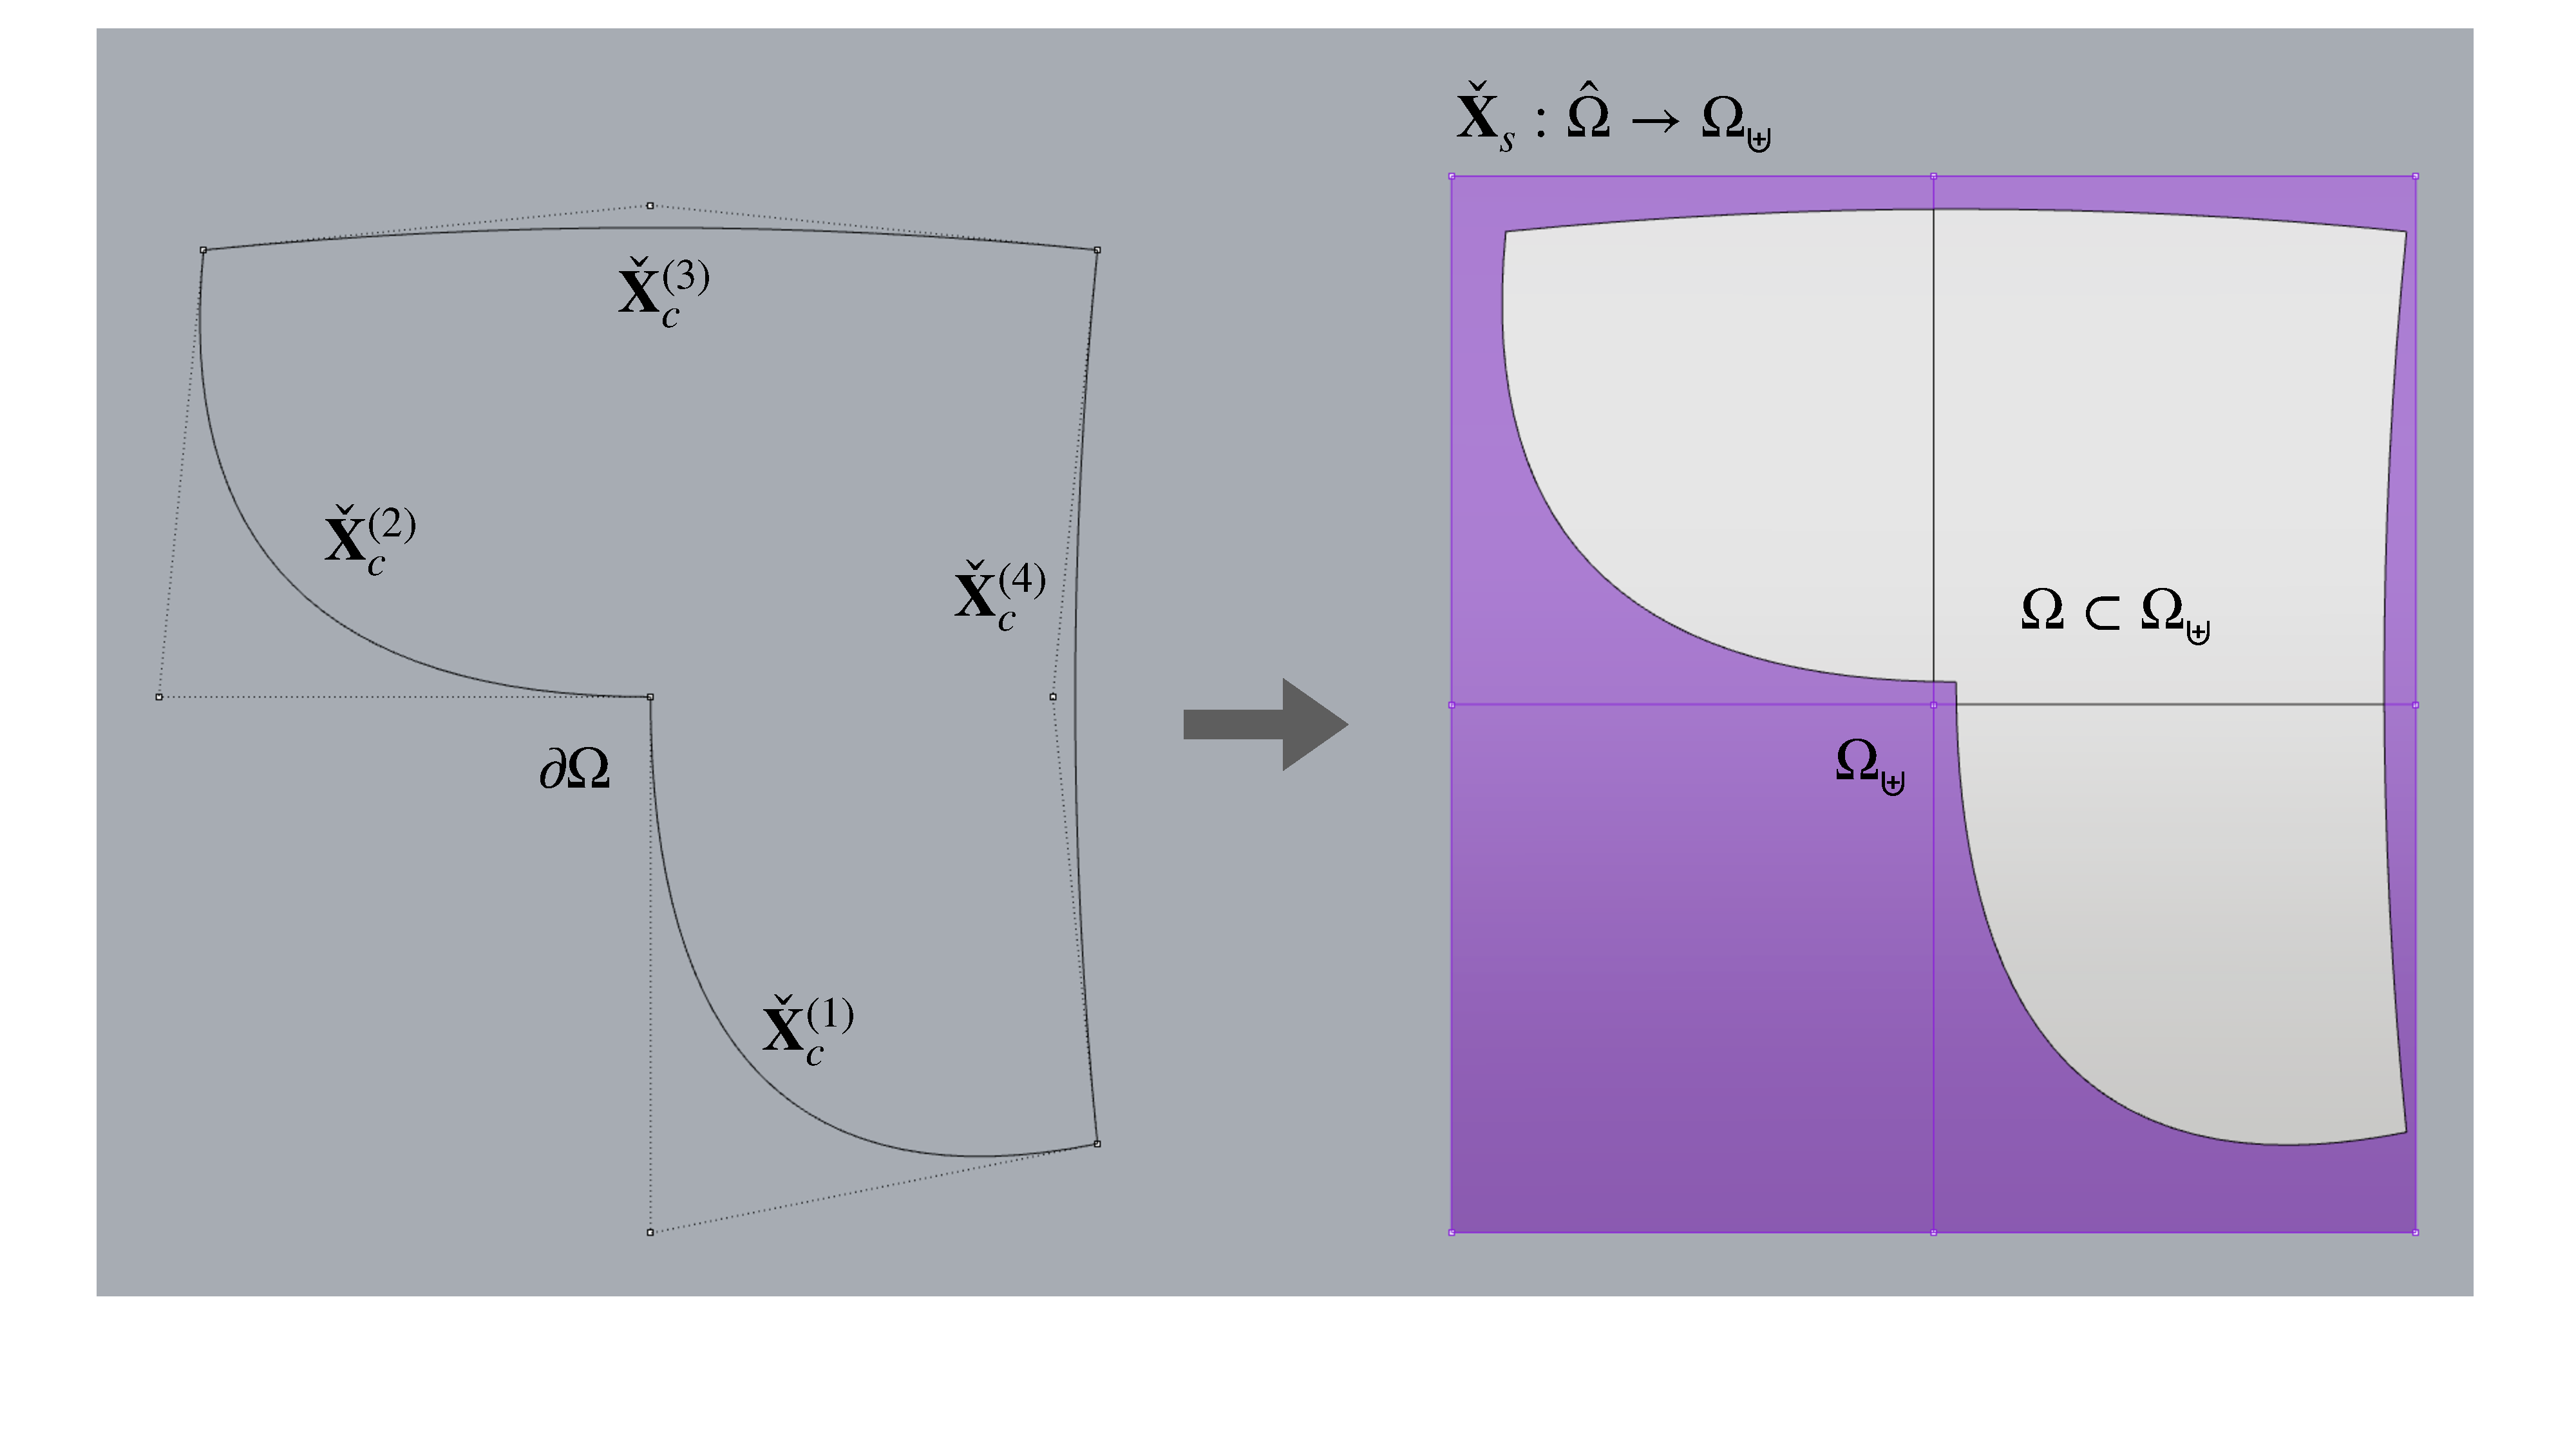
\includegraphics[scale=0.25]{Chapter5/Pictures/trimmed_dom}
    \caption{Parameterisation with trimmed domain }
    \label{fig:trimmed_dom}
\end{figure}


For the definition of a trimmed domain, since only essential part of the mapping that defines the domain from the parametric space to the physical space is considered, it does not place severe restriction over the complete parametric space to be mapped to the domain, illustrated in. This can be better in the context of designing where a surface can be loosely defined to contain a closed curve, but may not be suitable for defining $\bm \Phi$. One could say that for $\Omega \subset \Omega_{\uplus}$, with $\Omega_{\uplus}$ parameterised by $\bm X$, and given the bases $\bm \phi_\mathrm{i}:= \bm R_{i,j,k}(\mathbf{\Xi}) \circ \bm{X}^{-1}$, only the bases $\bm \phi_\mathrm{i}$ defining $\Omega$ can be considered for approximation. 
This is essentially the approach of the immersed methods, where typically the bases $\bm \phi_\mathrm{i}$ defining $\Omega$ is distinguished with material properties at the quadrature points, along with local refinement at the boundary of $\Omega\subset\Omega_{\uplus}$ through hierarchical refinement. Though immersed methods can have more flexibility in defining ${}_h \bm V$, we do not focus on such approaches owing to its novelty which can require immense time to develop.
 We purely focus on defining $\bm X:\hat\Omega\rightarrow\Omega$ which can be called body-fitted parameterisation. 
 The point is that to achieve body-fitted injective parameterisation for any shape as initial parameterisation can be too demanding from purely the perspective of CAD (Fig. (Fig. \ref{fig:body_neg}). 
 
 \begin{figure}[h!]
    \centering
    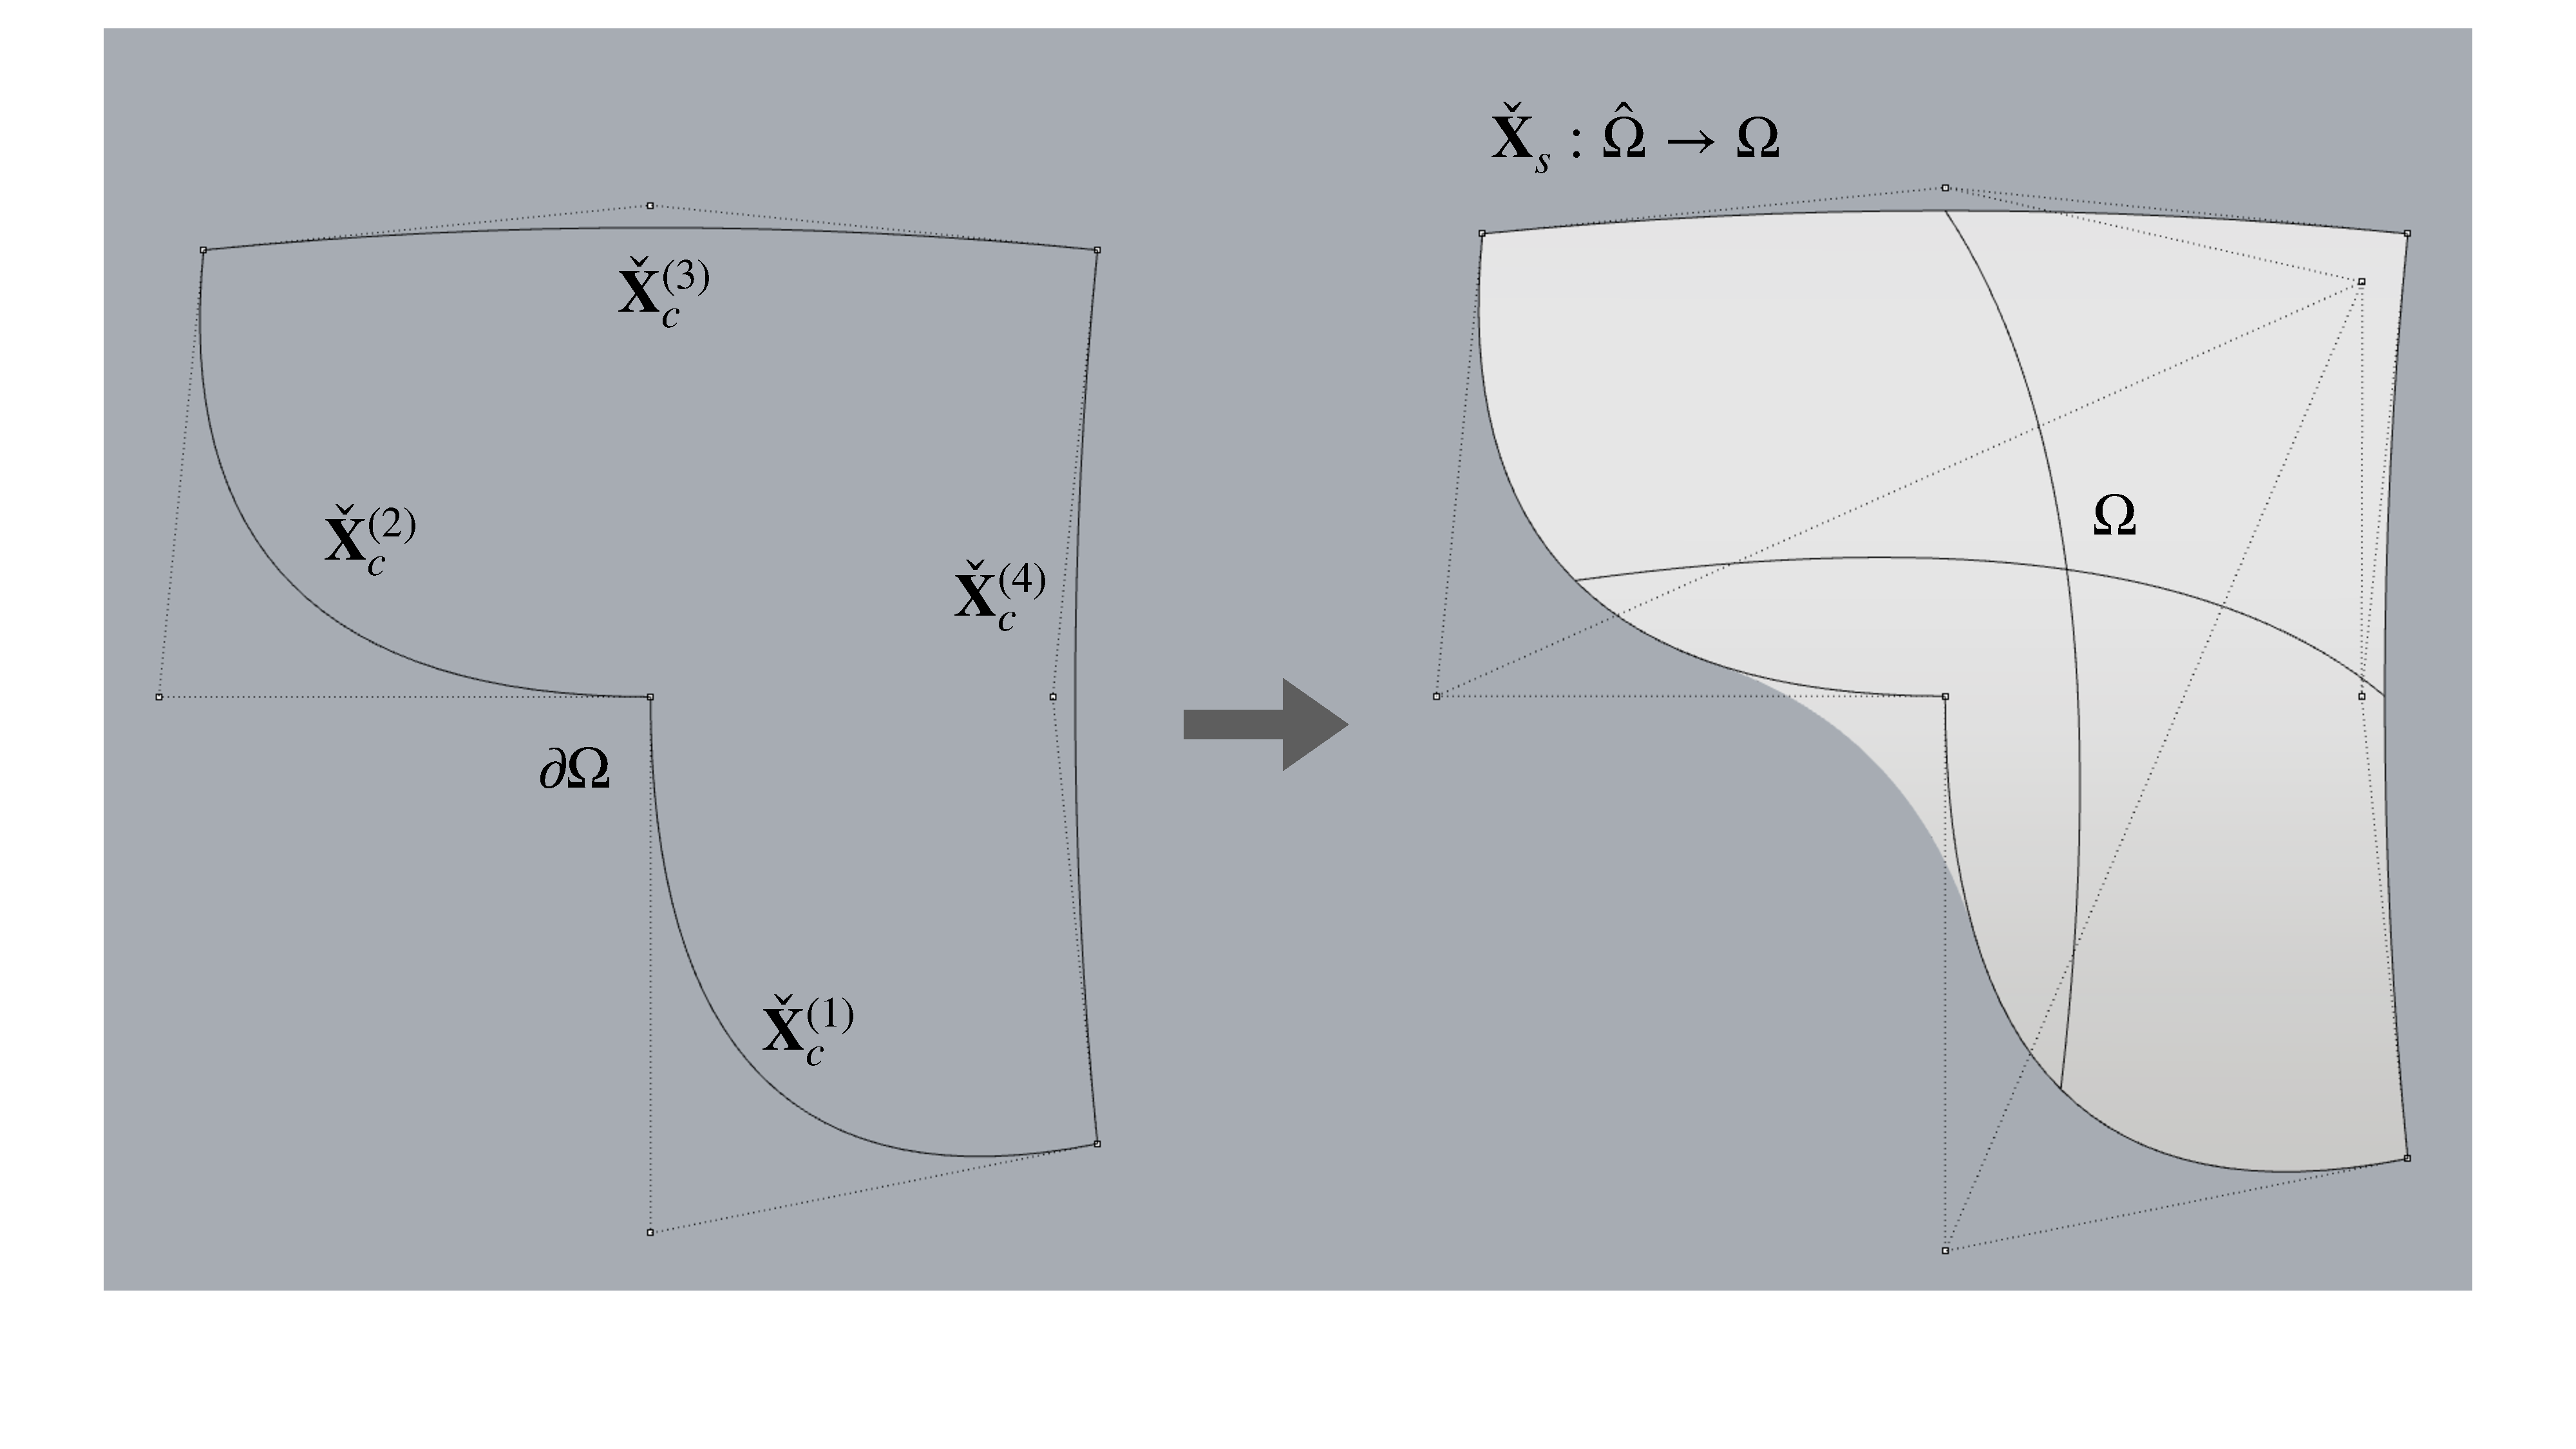
\includegraphics[scale=0.25]{Chapter5/Pictures/body_neg}
    \caption{Body-fitted non-injective parameterisation }
    \label{fig:body_neg}
\end{figure}


%Typically, the boundary of a domain is parametrised with lesser control points as parameters to define shapes, where to achieve an initial parameterisation given the boundary parameterisation can be sometimes impossible with lesser control points. 
For complex shapes, it is typically preferred to define analysis-suitable parameterisation directly, rather from a prior definition of initial parameterisation, where analysis-suitable parameterisation with sufficient refinement can be well suited to define injective parameterisation. 
From the perspective of CAD, this makes no difference as along as body-fitted injective parameterisation is achieved and hence, sometimes, no distinguish can necessarily be made between initial and analysis-suitable parameterisations (Fig. \ref{fig:body_pos}). 

 \begin{figure}[h!]
    \centering
    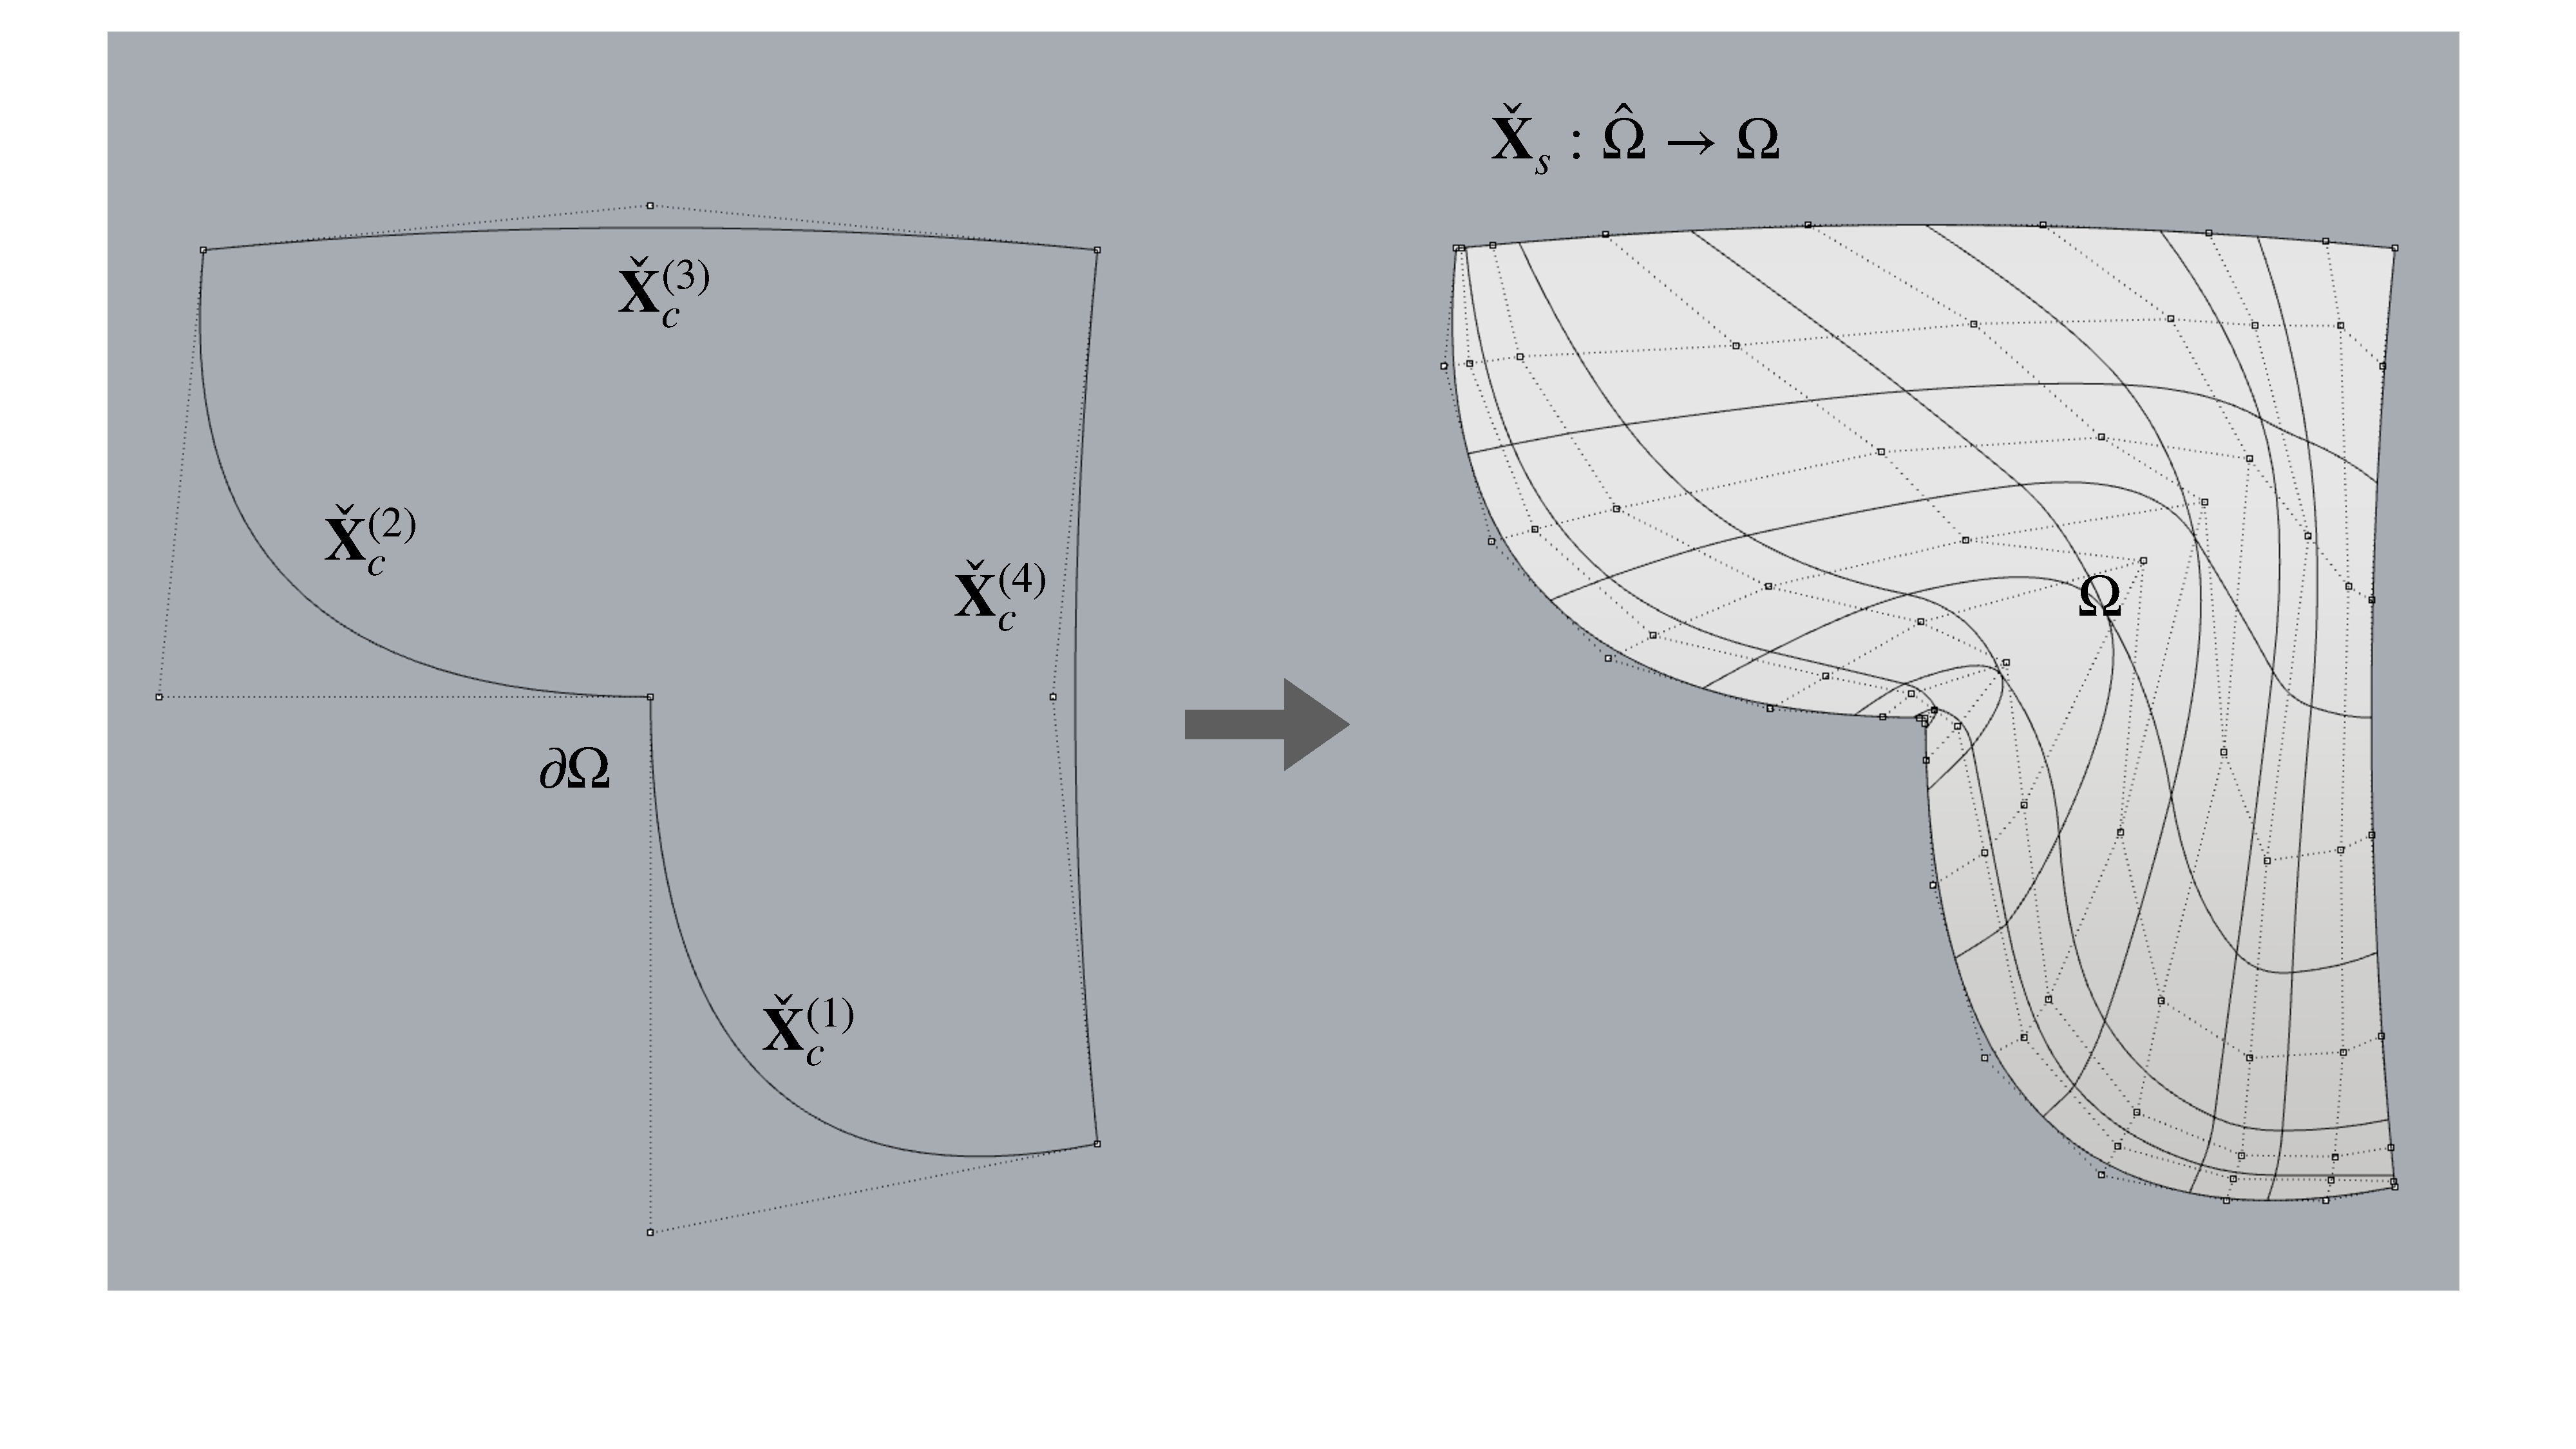
\includegraphics[scale=0.25]{Chapter5/Pictures/body_pos}
    \caption{Body-fitted injective parameterisation}
    \label{fig:body_pos}
\end{figure}

%At least for the definition of the boundary, we must talk about initial parameterization, in our case, with the chosen approach for parameterisation, for all parameterisation %Hence, expecting an initial parameterisation as body-fitted parameterisation for CAD can be very demanding, since for more complicated shapes it typically requires non-linear optimisation to find an injective body-fitted parameterisation.
%We stick with the narration of defining initial parameterisation prior to analysis-suitable parameterisation, since with the considered definition of shapes, it is possible to distinguish initial and analysis-suitable parameterisations, through there may not be an explicit advantage of this narration in our case.
Nevertheless, given the complexity of defining initial or analysis-suitable parameterisation, it is seen as a more robust strategy to define ${}_h \bm V$ compared to classical FEM. 
It should also be reminded that a complex domain can also be defined through multiple patches, where each patch corresponds to body-fitted parameterisation. But this also requires a more robust strategy to split a complex domain in to patches for any arbitrary definition of shape, at least for a fixed topology.
Nevertheless, we adapt multi-patch parameterisation as a strategy for local refinement and sub-structuring in optimisation.\\

For the scope of this thesis, we consider discrete Coon's patch method as a preliminary approach for the parameterisation part of the Bayesian shape optimisation framework. The idea is to adapt a more advanced parameterisation strategy for future evolution of the framework.\\



The parameterization of$ \bm {\check{X}}_{s}^{(\mathrm p)}(\xi,\eta)$ with the above four curves \eqref{curves_bound} by discrete Coon's patch method can be given as

\begin{multline}
    \bm {\check{X}}_{s}^{(\mathrm p)}(\xi,\eta) =\bm {\check{X}}_{c}^{(1)}(s)(1-\xi)+\bm X_c^{(3)}(u)(\xi)+\bm {\check{X}}_{c}^{(2)}(t)(1-\eta)+\bm X_c^{(4)}(v)(\eta)\\-\bm {\check{X}}_{c}^{(1)}(0)(1-\xi)(1-\eta) - \bm  X_c^{(1)}(1)(1-\xi)(\eta)\\ -\bm {\check{X}}_{c}^{(3)}(0)(\xi)(1-\eta) -\bm {\check{X}}_{c}^{(3)}(1)(\xi)(\eta)
\end{multline}

where the Coon's patch method is an explicit linear method and hence computationally efficient in realising parameterisation, but the method doesn't guarantee injective mapping. 
In our experience, the shapes realised through Coon's patch method that doesn't satisfy injective mapping are largely too conceptual for pad shapes and hence, given the complexity of realising parameterisation for such shapes, we only stick with the shapes realised through Coon's patch method for which injective property is satisfied.\\

In the scope of shape optimisation,$ \bm {\check{X}}_{s}^{(\mathrm p)}(\xi,\eta)$ can be defined as the function to be optimised, on which constraints can be imposed.
We define Constraint set 1, which contains constraints intrinsic of the boundary curves \eqref{curves_bound}. For simplicity owing to the preliminary definition of framework, in order to limit the parameters in optimization, we restricted the degree of each curve to $2$ and hence, this leads to the surface$ \bm {\check{X}}_{s}^{(\mathrm p)}(\xi,\eta)$ with the property $p=q=2$, and each curve is defined only through three control points which are just enough to define a curve of degree $2$. 
Furthermore, the optimisation is defined only for the position of the control points $\bm{P}_{i,j}$ for $w_{i,j} =1$ \eqref{NURBS_c}, i.e, we considered the optimization of the NURBS geometry only through affine transformation without considering projective transformation.\\
 
While the end control points will be constrained relative to the disc domain, given in Constraint set 3, we impose constraint on the mid-control point of each curve segment. The control points for any curve segment can be expressed as $\bm P_1$, $\bm P_2$ and $\bm P_3$, where $\bm P_1$ and $\bm P_3$ define the end control points. If the initial configuration of the curve can be expressed as a line segment $\overline{\bm P_1\bm P_3}$ with $\bm P_2 = \frac{\bm P_1+\bm P_3}{2}$, then the constraint on $\bm P_2$ can be expressed relative to the initial configuration as $\bm P_2 \perp \overline{\bm P_1\bm P_3}$\\


Constraints between curve segments are given as Constraint set 2 which contains constraints to confirm injective mapping, which also implicitly preserves topology.
Injective parameterisation can be said to be achieved if $ |\bm J( \bm {\check{X}}_{s}(\xi,\eta) )|$ does not vanish on all $\hat{\Omega}$.
With the mid-control points constrained, the set of constraints for testing this condition was realised geometrically, given as\\
 
{
Constraint set 2: 
\begin{multline}
   \quad \{\bm X_c^{(1)}(s) \cap\bm {\check{X}}_{c}^{(2)}(t)\}\cup \{\bm X_c^{(3)}(u) \cap\bm {\check{X}}_{c}^{(4)}(v)\}\cup \{\bm X_c^{(1)}(s) \cap\bm {\check{X}}_{c}^{(3)}(u)\}\cup\\
   \{\bm X_c^{(1)}(s) \cap\bm {\check{X}}_{c}^{(4)}(v)\} \cup \{\bm X_c^{(2)}(t) \cap\bm {\check{X}}_{c}^{(3)}(u)\} \cup \{\bm X_c^{(2)}(t) \cap\bm {\check{X}}_{c}^{(4)}(v)\} = \emptyset\\ 
\forall s,t,u,v \in (0,1)\\
\\
\{\bm X_c^{(1)}(0)(1-\xi)+\bm X_c^{(3)}(0)(\xi)\} \cap \{\bm X_c^{(1)}(0+\Delta s)(1-\xi)+\bm X_c^{(3)}(0+\Delta u)(\xi)\} = \emptyset\\
\{\bm X_c^{(1)}(1)(1-\xi)+\bm X_c^{(3)}(1)(\xi)\} \cap \{\bm X_c^{(1)}(1-\Delta s)(1-\xi)+\bm X_c^{(3)}(1-\Delta u)(\xi)\} = \emptyset\\
\{\bm X_c^{(2)}(0)(1-\eta)+\bm X_c^{(4)}(0)(\eta)\} \cap \{\bm X_c^{(2)}(0+\Delta t)(1-\eta)+\bm X_c^{(4)}(0+\Delta v)(\eta)\} = \emptyset\\
\{\bm X_c^{(2)}(1)(1-\eta)+\bm X_c^{(4)}(1)(\eta)\} \cap \{\bm X_c^{(2)}(1-\Delta t)(1-\eta)+\bm X_c^{(4)}(1-\Delta v)(\eta)\} = \emptyset\\
\forall \xi,\eta \in [0,1]
\end{multline}
}
where $\Delta$ represents an arbitrary small variation. The first constraint avoids intersection between the curves except for the end points. Satisfying the first constraint which guarantees a fixed topology does not assure injective parameterisation through Coon's patch method, for which the last set of four constraints are necessary.  The last set of four constraints implicitly avoid concave intersection between the curves. Given that the curves do not intersect except for convex intersection at the end points, and with constraints on the mid-control points, injective parameterisation can be achieved with Coon's patch method. \\
% Alternate way to realise

Further, the definition of the pad surface to be with in the bounds of the disc surface is given through a box constraint as follows\\

Constraint set 3: \\
\begin{equation}
    (\bm X_{s(lb)} \leq \bm X_s^{(\mathrm p)}(\xi,\eta) \leq \bm X_{s(ub)}) :   \{[\bm X_{c(lb)}^{(i)},\bm X_{c(ub)}^{(i)}]\} \cap   \{[\bm X_{c(lb)}^{(j)},\bm X_{c(ub)}^{(j)}]\} = \emptyset  
\end{equation}

where the choice of $\bm X_{s(lb)}$ and $\bm X_{s(ub)}$ depends on the design choice for the domain of the disc to be in contact with the pad. Further, the box constraint is adapted to limit the redundancies in geometric description i.e, to limit the scope for a given shape to be defined in more than one way with in the same design space. To avoid this type of redundancy, we restricted the domain through box constraints for at least two curves $\bm X_{c}^{(i)}(.)$ and $\bm X_{c}^{(j)}(.)$ of the four curves, such that the intersection of their domains is a null set. This leads to restriction of the design space with compromise on reducing the redundancies. Hence, we avoided some of the redundancies on empirical notion, such that the restricted design space has lesser meaningful designs. This maybe an interesting anomaly to investigate, since the redundancies may lead to larger design space with more severe multi-modality.\\   

We further impose an inequality constraint in order to avoid designs with smaller contact surface, given as\\

Constraint 4: \\
\begin{equation}
    Area(\bm X_{s}^{(\mathrm p)}(\xi,\eta)) \geq A_{min}
\end{equation}

where $Area(\bm X_{s}^{(\mathrm p)}(\xi,\eta)): \int_{\xi}\int_{\eta}|\frac{\partial \bm {\check{X}}_{s}^{(\mathrm p)}}{\partial \xi} \times \frac{\partial \bm {\check{X}}_{s}^{(\mathrm p)}}{\partial \eta}|d\xi d\eta$ and the choice of $A_{min}$ depends on the minimum contact surface area that is required on the Pareto-front, since maximization of $Area(\bm X_{s}^{(\mathrm p)}(\xi,\eta))$ is defined to be one of the objectives.\\

The definition of the shape of$ \bm {\check{X}}_{s}^{(\mathrm p)}(\xi,\eta)$ through this strategy means that there is no requisite for a reference configuration to define optimization, but instead the pad shapes are defined through random generation of curves with $C^0$ continuity between them. We assume that this restricts bias to any specific shape and hence encouraging more randomness in defining a meaningful geometry. 
This highly restricts the use of gradient-based approaches for optimization, since the constraints are also black-box and may have discontinuities. 
Some of the limitations can also be attributed to lack of exploring classical shapes such as the annulus sector pad shapes in our application even though such shapes are already a subset of the the design space defined. The randomness in the definition of shapes can lead to higher probability of failure for the constraints, and hence more constraint evaluation in optimisation.\\

Finally, the objectives for the Multi-objective optimization can be posed as optimization of the following functionals: 

\begin{itemize}
    \item Objective 1:
$min \, C_{\mathsf s}(\bm X_{s}^{(\mathrm p)}(\xi,\eta)\,|\,\Im(\bm \Lambda(\bm X^{(\mathrm{d-p})})\in[10KHz,13KHz])$
    \item Objective 2:
$max \, Area(\bm X_{s}^{(\mathrm p)}(\xi,\eta))$
\end{itemize}

%Objective 1:
%$min \, C_s(\bm X_{s}^{(\mathrm p)}(\xi,\eta))\,|\,\Im(\Lambda(\bm X_{s}^{(\mathrm p)}(\xi,\eta)))\in[10KHz,13KHz]$

%Objective 2: 
%$max \, Area(\bm X_{s}^{(\mathrm p)}(\xi,\eta))$

where the optimisation of the functionals are defined over the space of NURBS functions. Since we fixed the order and the number of control points of the NURBS surface$ \bm {\check{X}}_{s}^{(\mathrm p)}(\xi,\eta)$, the optimisation is restricted to a fixed number of control points.\\ 

\subsection{Isogeometric parameterization and refinement strategies for the disc-pad system domain with contact considerations} \label{subsec:iso_ref_strat}
{For the following, we do not focus on the mesh sensitivity for CEA or the stability criterion $C_{\mathsf s}$, but instead the below refinement strategies can be seen as to realise the classical mesh refinement considerations for a contact problem, where more elements are typically defined on $\Gamma_C$ and at the vicinity of $\partial \Gamma_C$ to capture more accurately the contact characteristics and the strong solution gradient. This is especially more challenging with local refinement for NURBS parameterization, hence we expose here some strategies to achieve local refinement. Empirically, the refinement at $\Gamma_C$ and around $\partial \Gamma_C$ seems to effect the results of CEA and converges with sufficient refinement, but a more qualitative assessment of the sensitivity has not been developed here, since it requires a detailed study of not only the refinement but also the contact formulation and  the nature of modelling contact stiffness.}\\

The planar parameterization$ \bm {\check{X}}_{s}^{(\mathrm p)}$ can be easily extended to define $\Omega^{(\mathrm p)}$ as $\bm X_{v}^{(\mathrm p)}$ considering the thickness of the pad through the tensor product definition \eqref{NURBS_v}, given a NURBS line along the thickness. 
The disc domain $\Omega^{(\mathrm d)}$ was realised by multi-patch parameterization $\bm X_{v}^{(\mathrm d)} := \bm X_{v}^{(\mathrm d_1)} \cup \bm X_{v}^{(\mathrm d_2)}$ to achieve local refinement on $\Gamma_C^{(\mathrm d_2)}$. {The surface parameterization for the disc patches$ \bm {\check{X}}_{s}^{(\mathrm d_1)}$ and$ \bm {\check{X}}_{s}^{(\mathrm d_1)}$ can be achieved through the concept of revolved surface, detailed in \citep{Piegl1995TheNB}, which assures robust injective parameterisation since the curve to be revolved is a straight line perpendicular to the disc axis, given that the straight line does not pass through the axis. The planar parameterizations$ \bm {\check{X}}_{s}^{(\mathrm d_1)}$ and$ \bm {\check{X}}_{s}^{(\mathrm d_2)}$ can be extended to $\bm X_{v}^{(\mathrm d_1)}$ and $\bm X_{v}^{(\mathrm d_2)}$ respectively, similar to achieving $\bm X_{v}^{(\mathrm p)}$}.\\

For any refinement, the space for parameterisation remains the same i.e, $(\xi,\eta,\zeta) \in [0,1]^3$ and the refinement is defined only through manipulation or addition of knots and control point to achieve an analysis-suitable parameterisation. 
After an analysis-suitable parameterisation, to take in to account of the additional control points and the manipulated knot vectors, $\bm X_{v}^{(\mathrm p)}$ and $\bm X_{v}^{(\mathrm d)}$ can be expressed as $\overline{X}_{v}^{(\mathrm p)}$ and $\overline{X}_{v}^{(\mathrm d)}$. 
Hence, the NURBS bases associated with $\overline{X}_{v}^{(\mathrm p)}$ and $\overline{X}_{v}^{(\mathrm d)}$ are used to define the space for approximation in isogeometric approach, detailed in Section \ref{cont_des}. It should be noted that often analysis-suitable parameterisation is achieved directly in the scope of defining an injective parameterisation, since for complex shapes, analysis-suitable parameterisation with sufficient refinement can be well suited to define injective parameterisation.
Hence, often no distinguish can be made between initial and analysis-suitable parameterisations, since the definition of body-fitted initial parameterisation in the context of CAD may already demand sufficient refinement to achieve even an elementary injective  parameterisation. Since we only choose designs for which injective parameterisation exists with Coon's patch method, it is safe to say that for any analysis-suitable injective parameterisation achieved through Coon's patch method, initial injective parameterisation can also be achieved by Coon's patch method. Hence, we talk in the context that initial parameterisation of CAD does not have sufficient refinement  to define the space ${}_h\bm V$ and hence we explicitly define analysis-suitable parameterisation through refinement.\\

%In the following, we show the strategy adapted to achieve  analysis-suitable parameterizations $\overline{X}_{v}^{Pad}$ and $\overline{X}_{v}^{Disc}$ in shape optimization.
 Normally across the boundary $\partial\Gamma_C$ of a contact domain $\Gamma_C$, there is drastic change in the solution gradient and hence, the parameterization needs special attention owing to the continuity of the NURBS bases. The tensor product property of the NURBS gives further challenge for local refinement which is usually desired on $\Gamma_C$. These challenges can be largely overcome by adaptation of NURBS bases to T-splines \citep{BAZILEVS2010229} or THB-splines \citep{GIANNELLI2012485}, but requires extensive adaptation. Hence, we defined a multi-patch parameterization strategy through collocation and projection of  properties defined on control points between two merging surfaces, which was simple and efficient for our application with fewer adaptation. Even though the considered multi-patch approach only considers $C^0$ solution continuity between the patches, the post-processing of the mode shapes show sufficient smoothness in displacement field across the patches, shown in Figure \ref{fig:MP_anatom}.\\

\begin{figure}[h!]
    \centering
    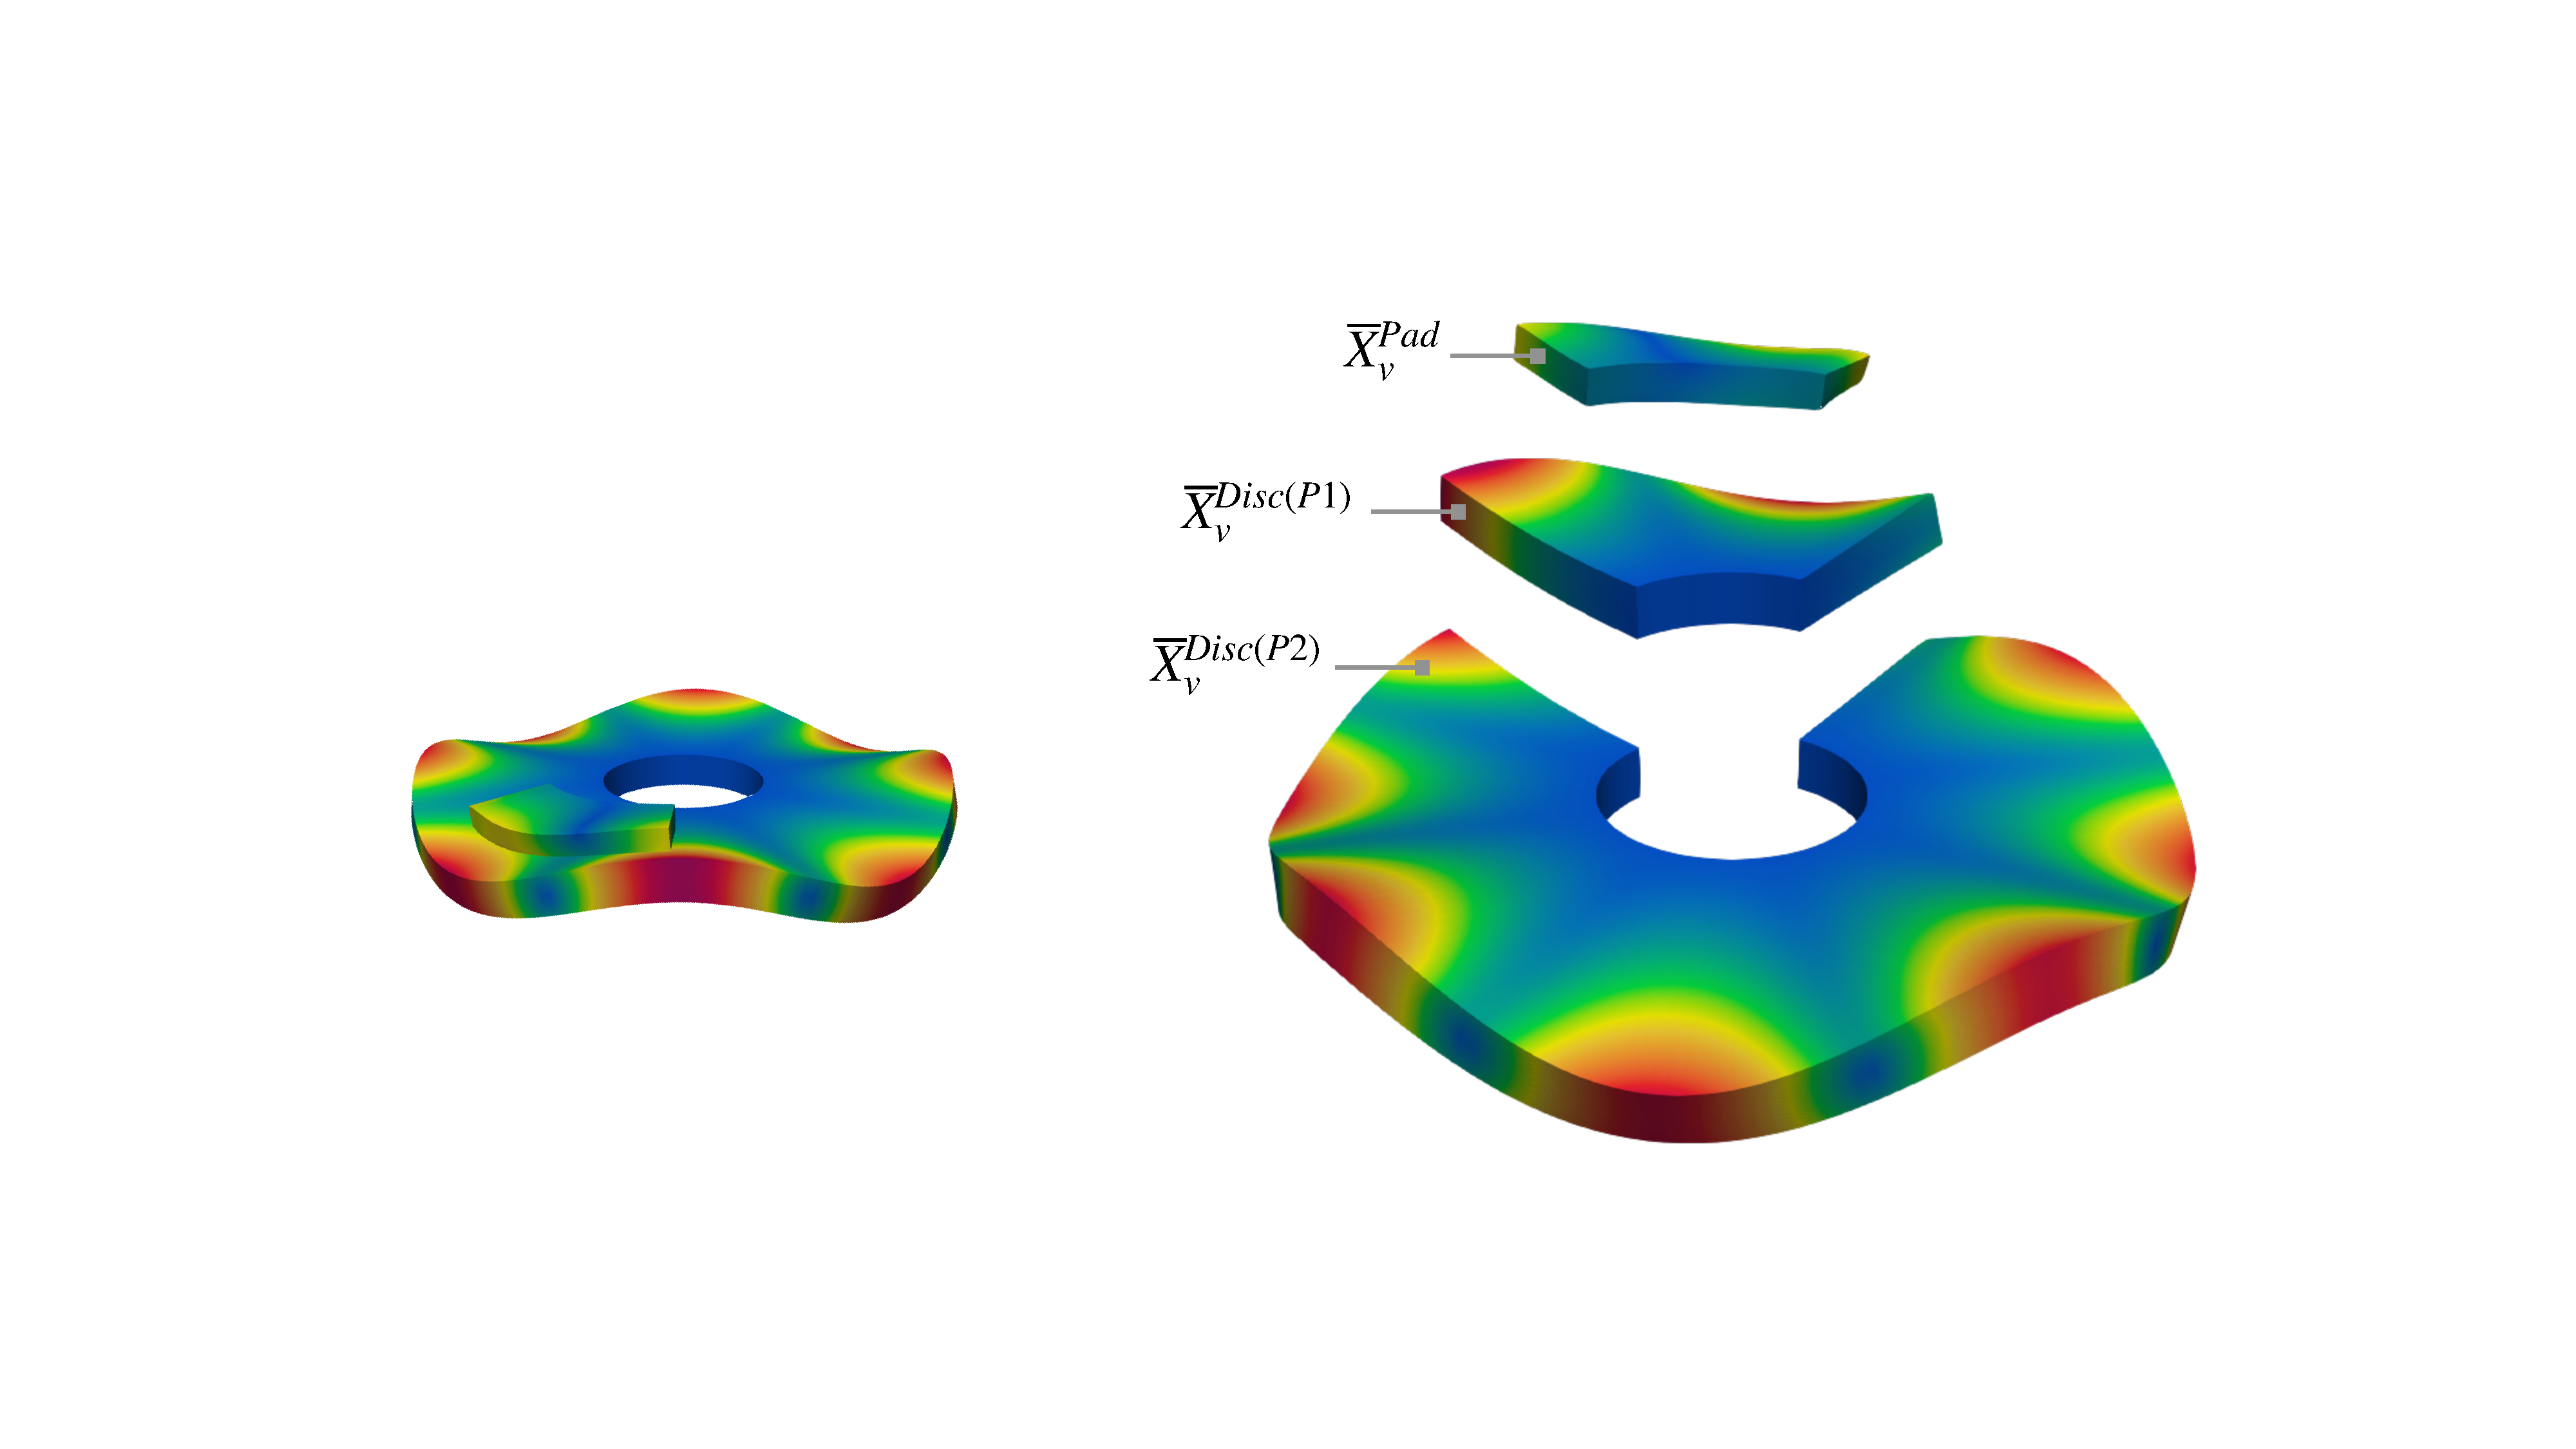
\includegraphics[scale=0.28]{Chapter5/Pictures/MP.pdf}
    \caption{Anatomy of parameterization for the disc-pad system with arbitrary dimensions, shown here for Mode 9, Frequency: 3630 Hz}
    \label{fig:MP_anatom}
\end{figure}

%We adapted some techniques which was well suited for our domain and problem of interest. 
The multi-patch parameterization of $\Omega^{(\mathrm d)}$ to break the NURBS tensor product definition is shown in Figure \ref{fig:multi-patch_disc}, where one patch  $\overline{X}_{v}^{(\mathrm d_1)}$ contains the contact domain $\Gamma_{C}^{(\mathrm d_1)}$ defined through a fine mesh by $h$-refinement and the other patch $\overline{X}_{v}^{(\mathrm d_2)}$ with a relatively coarse mesh sufficient to capture the required dynamic properties. And different strategies were used to reduce the solution smoothness induced by the continuity of the NURBS approximation across the boundary $\partial \Gamma_{C}^{(\mathrm d_2)}$ where typically strong solution gradient exists. For pad shapes where the knot lines on  $\overline{X}_{v}^{(\mathrm d_1)}$ can be aligned with $\partial\Gamma_{C}^{(\mathrm d_1)}$, $h$-refinement can be used with finer refinement around $\partial\Gamma_{C}^{(\mathrm d_1)}$, while the contact domain $\Gamma_{C}^{(\mathrm d_1)}$ itself is discretized by $h$-refinement through a relatively coarse mesh compared to the refinement around $\partial\Gamma_{C}^{(\mathrm d_1)}$, but finer than the rest of the domain. For pad shapes where the knot lines on $\overline{X}_{v}^{(\mathrm d_1)}$ cannot be aligned with the boundary $\partial\Gamma_{C}^{(\mathrm d_1)}$, we purely relied on $h$-refinement with much finer refinement. For the shape optimization, we used the later strategy due to random definition of shapes. \\


\begin{figure}[h!]
    \centering
    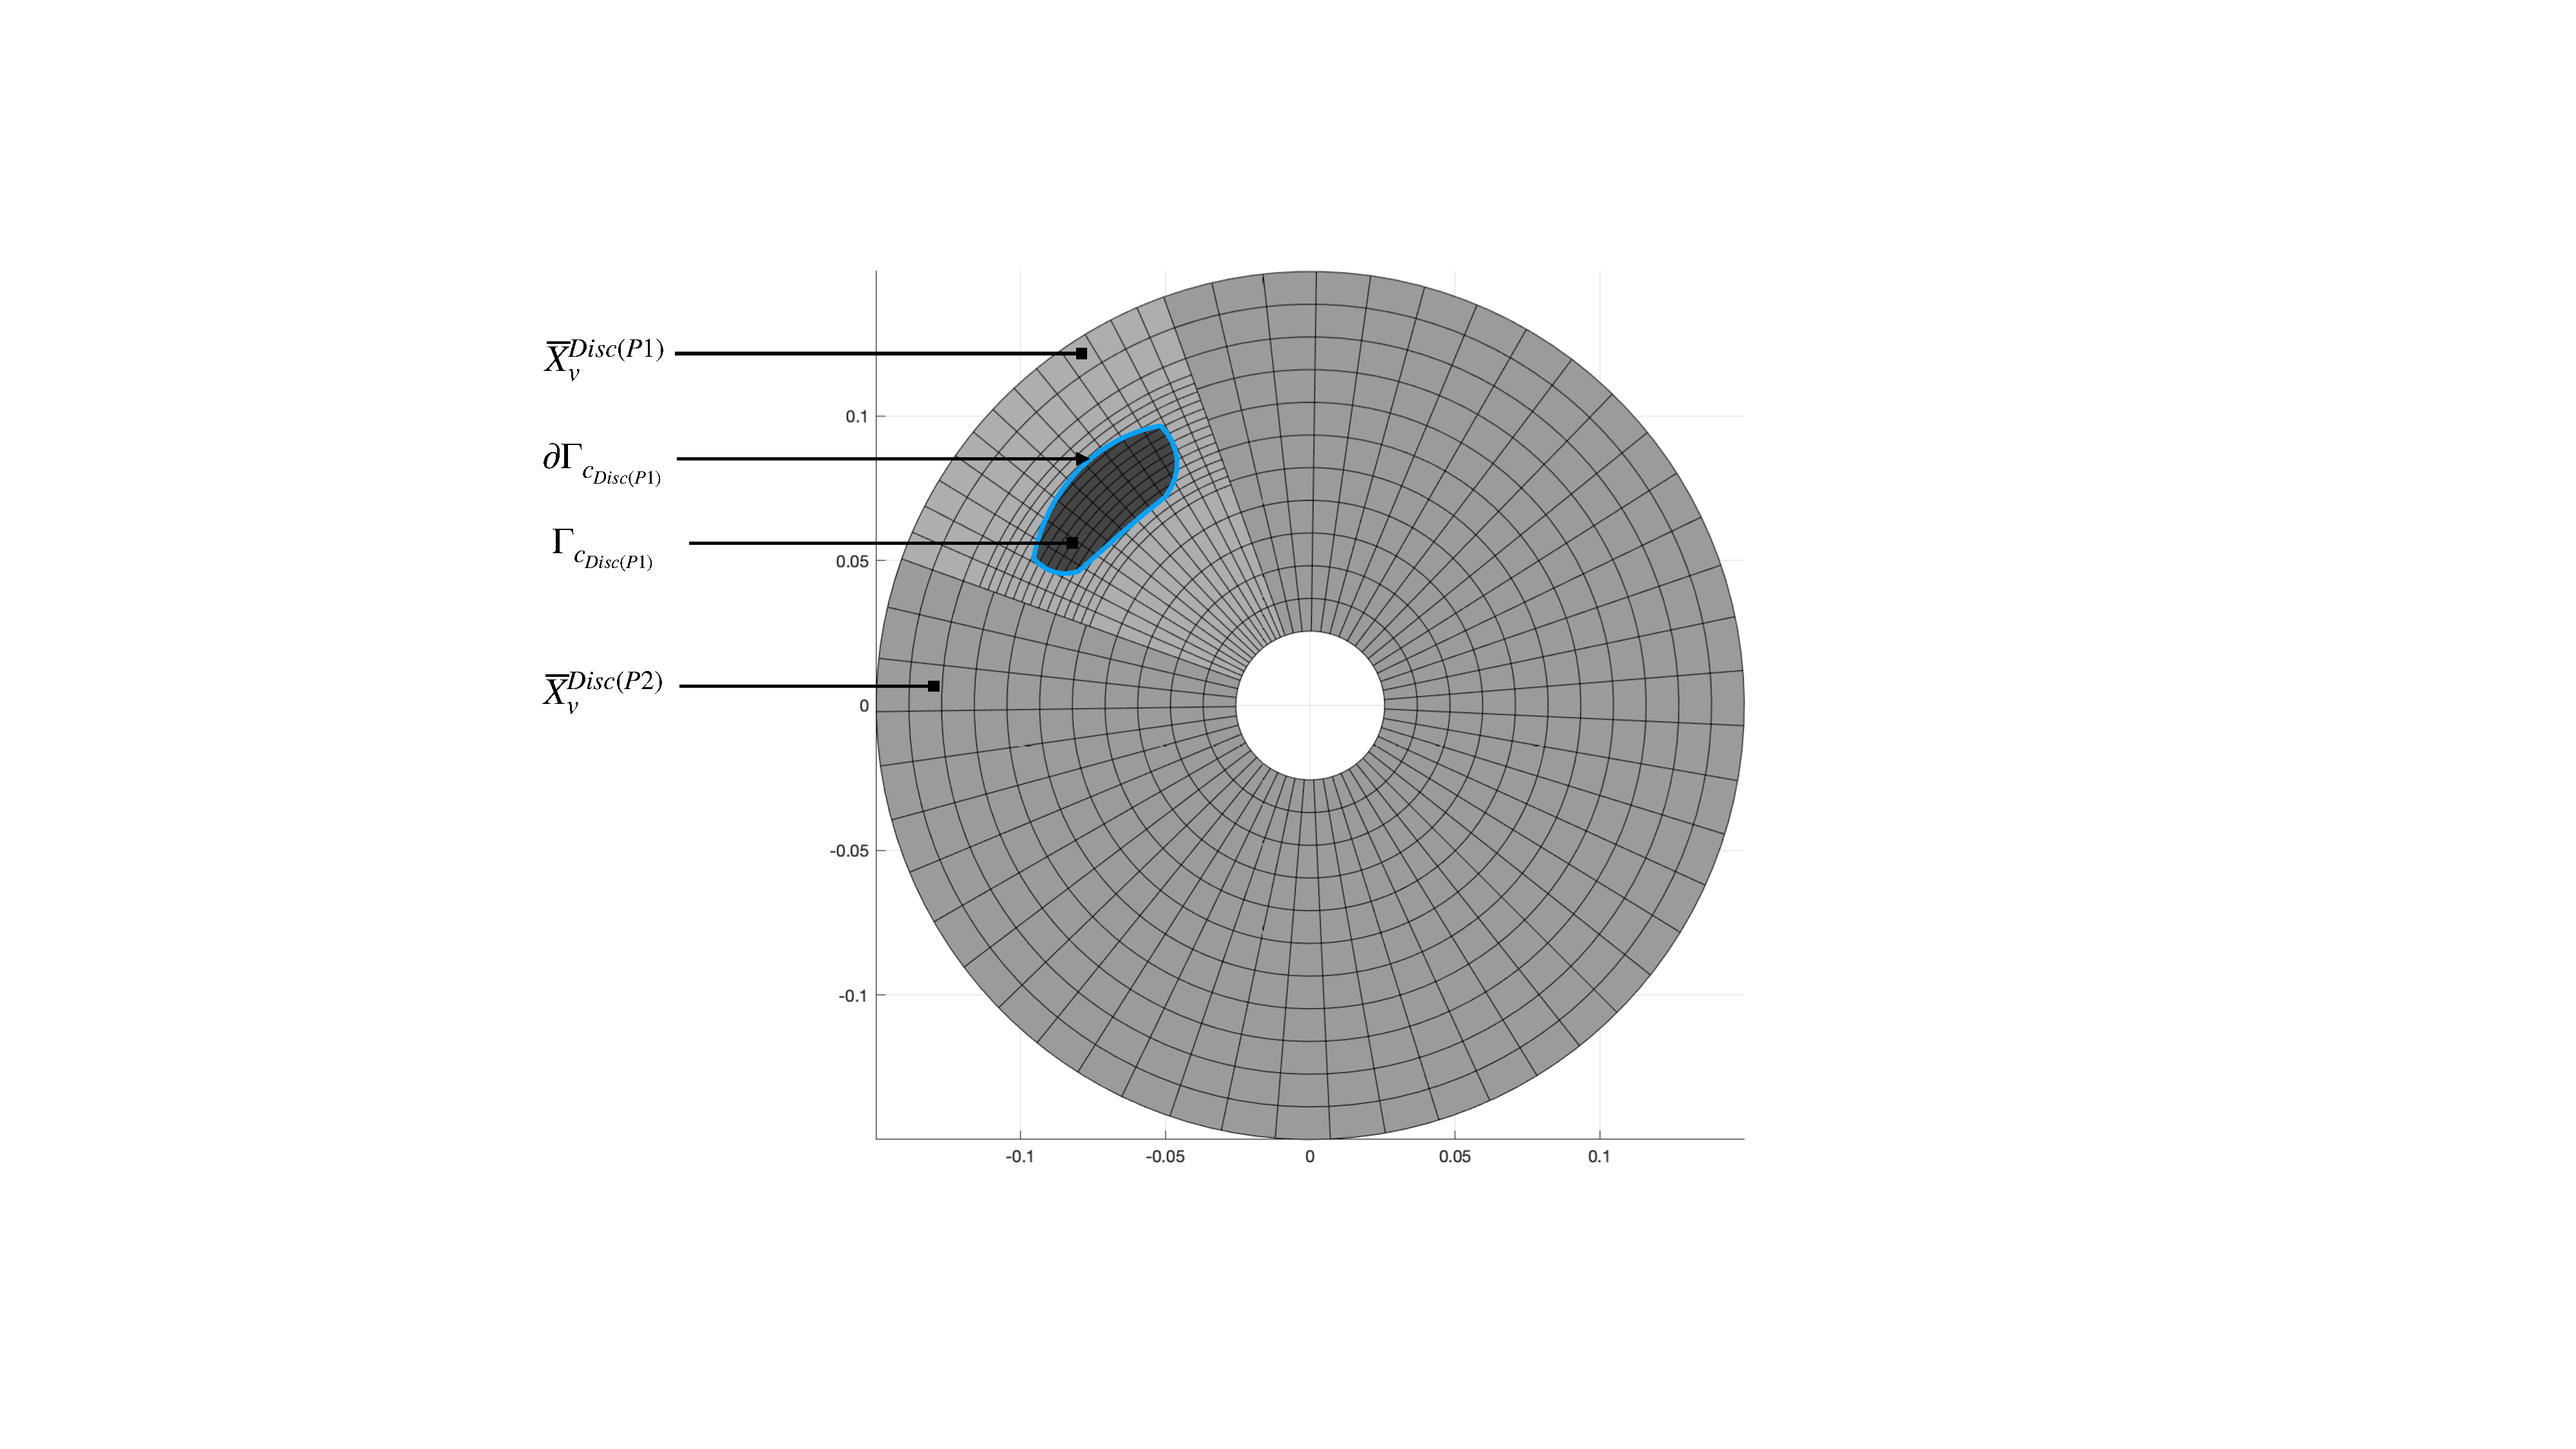
\includegraphics[scale=0.3]{Chapter5/Pictures/ran3.pdf}
    \caption{Multi-patch parameterization of $\Omega_{Disc}$ as $\overline{X}_{v}^{Disc}:=X_{v}^{Disc(P1)}(\xi,\eta,\zeta) \cup X_{v}^{Disc(P2)}(\xi,\eta,\zeta)$, with $h$-refinement at the contact region $\Gamma_{c_{Disc(P1)}}$.}
    \label{fig:multi-patch_disc}
\end{figure}

%As aforementioned, the pad is defined through a single patch parameterization $X_{v}^{Pad}(\xi,\eta,\zeta)$.
%In the optimization loop, for arbitrary definition of pad shapes, the parameterization was adapted for change in shape through $r$-refinement strategy i.e, the number of control points except for their positions are fixed. 
%Further, in the optimization loop, the dimension of the disc patches were adapted for changes in $\Gamma_{c_{Disc(P1)}}$ to realize a more restrictive local refinement on $\Gamma_{c_{Disc(P1)}}$ and across $\partial\Gamma_{c_{Disc(P1)}}$. Hence, the knot vectors were also adapted to have uniform spacing of knots for a given region irrespective of the change in the dimension of the patches. 

%While the multi-patch parameterization of $\Omega^{(\mathrm d)}$ makes it computationally efficient with defining local refinement on $\Gamma_{C}^{(\mathrm d_1)}$ and across $\partial\Gamma_{C}^{(\mathrm d_1)}$, 


 
 

\subsection{Bayesian optimization}

Bayesian optimization is an effective strategy for optimising computationally expensive objective functions \cite{Shahriari}. 

We begin the following explanations without defining the specifics of modelling the probability $\mathcal{P}$ which is given as knowledge and considering the optimisation of a single function $f(\bm{x})$ for $\underset{\bm x \in \mathcal{X}}{min}\,f(\bm{x})$.
The idea is based on Bayes rule where the prior knowledge $\mathcal{P}(\mathcal{H})$ of the hypothesis $\mathcal{H}$ and the likelihood of the evidence $\mathcal{E}$ given the hypothesis, $\mathcal{P}(\mathcal{E}|\mathcal{H})$, are used to infer the posterior knowledge of the hypothesis given the evidence, $\mathcal{P}(\mathcal{H}|\mathcal{E})$, where the proportionality is expressed as follows

\begin{equation}\label{Baye1}
\mathcal{P}(\mathcal{H}|\mathcal{E}) \propto \mathcal{P}(\mathcal{E}|\mathcal{H})\mathcal{P}(\mathcal{H})
\end{equation}

 where $\mathcal{P}(\mathcal{H}|\mathcal{E})$ defines Bayesian inference. In our setting, the hypothesis $\mathcal{H}$  corresponds to the function $f(\bm{x})$ and the evidence $\mathcal{E}$ to $\mathcal{F}_{1:{\mathfrak{n}}}:\{f(\bm{x}_1),f(\bm{x}_2),\hdots,f(\bm{x}_{\mathfrak{n}})\}$ where $f(\bm{x})$ is sampled on $\mathcal{X}_{1:{\mathfrak{n}}}:\{\bm{x}_1,\bm{x}_2,\hdots,\bm{x}_{\mathfrak{n}}\}$, with $\mathcal{D}_{1:{\mathfrak{n}}}:\{\mathcal{X}_{1:{\mathfrak{n}}},\mathcal{F}_{1:{\mathfrak{n}}}\}$. This is typically known as function-space view, since the probability is defined on the space of functions. It can be hard to conceptualise such view with functions, but it is possible if one can imagine the existence of a function in a mere probabilistic sense such that the random draw from a probability distribution is a function.  The relation \eqref{Baye} can be expressed in this case as\\
 
 \begin{equation}\label{Baye}
\mathcal{P}(f(\bm{x})|\mathcal{D}_{1:{\mathfrak{n}}}) \propto \mathcal{P}(\mathcal{D}_{1:{\mathfrak{n}}}|f(\bm{x}))\mathcal{P}(f(\bm{x}))
\end{equation}

 
 %The posterior knowledge can be then used to infer the optimum of the function where the expensive computational model needs to be evaluated. The new evaluation is then used to update the  belief of the prior, and with the likelihood to infer a new posterior. The process is run subsequently for optimization with the expectation of reaching the global optimum for the function. The most common method to model the prior of a function is through Gaussian process, which also infers the posterior as Gaussian. This is more efficient since this presents the prediction and the uncertainty of the prediction, which provides a decisive knowledge to construct an acquisition function to sample more efficiently for optimization.\\

%The modelling of prior, and the inference of posterior, for a function to be approximated takes the role of surrogate modelling commonly known as Gaussian process regression or Kriging. There are different context through which the Gaussian process regression could be presented owing to its diverse origins. We present in the context of function space view of Gaussian processes, but the interested readers can refer to the following articles for more details  \citep{Rasmussen1}\citep{Forrester}. Followed by, we present an acquisition function where we adapted  Expected Improvement($EI$) that defines EGO \citep{Jones1998}.\\
 
The prior over a function, $\mathcal{P}(f(\bm{x}))$, is typically modelled through spatial correlation which is assumed to be known a priori, where the hypothesis is that a given function exhibits certain characteristics of spatial correlation which can be generalized globally. 
In other words, a prior belief is defined over the space of functions, such that the functions in the space largely exhibit certain characteristics of spatial correlation. % which the function to be optimised is believed to exhibit. 
 With the prior $\mathcal{P}(f(\bm{x}))$ defined, and given the likelihood of the points sampled on the function, $\mathcal{P}(\mathcal{D}_{1:{\mathfrak{n}}}|f(\bm{x}))$, the posterior knowledge of the function, $\mathcal{P}(f(\bm{x})|\mathcal{D}_{1:{\mathfrak{n}}})$, can be inferred from the relation \eqref{Baye}. 
 The posterior knowledge $\mathcal{P}(f(\bm{x})|\mathcal{D}_{1:{\mathfrak{n}}})$ is then used to infer the next point $\bm{x}_{\mathfrak{n}+1}$ to be sampled, depending on the strategy set for sampling in optimization. 
 The sampled point $\bm{x}_{\mathfrak{n}+1}$ is then used to update the belief of the prior $\mathcal{P}(f(\bm{x}))$ in the light of $\mathcal{D}_{1:{\mathfrak{n}+1}}$, and with the likelihood $\mathcal{P}(\mathcal{D}_{1:{\mathfrak{n}+1}}|f(\bm{x}))$ to infer a new posterior $\mathcal{P}(f(\bm{x})|\mathcal{D}_{1:{\mathfrak{n}+1}})$, which characterizes active learning. 
 The process is run subsequently with the prospect of finding the global optimum for the function through active learning, defines Bayesian optimization.\\

With the general idea defined for Bayesian optimization, at least in the context of optimizing a single function, we can now define the notion of modelling $\mathcal{P}$ which is typically defined through Gaussian process ($\mathcal{GP}$). 
While a Gaussian distribution defines distribution over a random variable or in the case of a multi-variate Gaussian distribution over random variables, a $\mathcal{GP}$ defines distribution over a function, such that each draw from a $\mathcal{GP}$ is a function. 
For some intuition of the following explanations, this can be thought in a discrete sense as all the points, of a function drawn from a $\mathcal{GP}$ as being related through a dependent multi-variate Gaussian distribution such that each point is a univariate Gaussian distribution over a value of the function.\\

The prior over a function can hence be defined as $\mathcal{GP}$ prior, where the advantage of modelling the prior as Gaussian means that it preserves the conditioning of the Gaussian prior given the likelihood to infer the posterior as Gaussian as well. This is advantageous for Bayesian optimisation, since inferring the posterior as Gaussian presents the prediction as mean and the uncertainty of the prediction as variance, which provides a decisive knowledge to construct an acquisition function to sample more efficiently.\
The $\mathcal{GP}$ posterior defined through Bayesian inference from conditioning a $\mathcal{GP}$ prior given the likelihood of the sampled points over the function, characterizes a regression model, known as $\mathcal{GP}$ regression. Hence, the meta-modelisation of the function $f(\bm{x})$ can be defined through $\mathcal{GP}$ regression. \\

%Hence, it can be said in a probabilistic sense that a function with large variation between two arbitrary points for a given distance defined by a metric characterises weak spatial correlation, than a function with smaller variation for the same distance. The comparison can only be defined probabilistically, since different parts of the function can exhibit different spatial correlation, which means that characterising a function with respect to spatial correlation can also only be probabilistic. Even though, the knowledge of spatial correlation is assumed to be known a prior, it is often determined from the of light of the sampled data.  
%From a function-space view, $\mathcal{P(H)}$ can be defined as distribution over functions, where the distribution largely corresponds to functions which exhibit certain characteristics of spatial correlation. 
 %More on the mathematical specifics for defining the prior probabilistically will be shown in the upcoming explanations.\\
 
%Given the prior defined through spatial correlation for a function, and with the points sampled on the function, the posterior knowledge of the function can be inferred from the relation \eqref{Baye}.
%The posterior knowledge is then used to determine the next point to be sampled, where the process of determining a sample point is typically achieved through optimising an acquisition function. More on the role of acquisition function in optimization will be discussed later. 
%The sampled point is then used to update the belief of the prior, and with the likelihood to infer a new posterior. 
%The process is run subsequently which defines Bayesian optimization with the expectation of reaching the global optimum for the function. This is helpful for computationally expensive functions when often the computational resources are limited, where applying the classical optimization strategies cannot converge with the reduced number of evaluations.\\

 %With the general idea behind Bayesian optimization at least in the context of single objective optimization, we can now define the notion of modelling $\mathcal{P}(.)$ which is typically defined through Gaussian: $\mathcal{N}({\mu},{\sigma}^2)$. 
% While a Gaussian distribution defines distribution over a random variable or in the case of a multi-variate Gaussian distribution over random variables, a Gaussian process $\mathcal{GP}$ defines distribution over a function. 
 %Hence, the prior over a function is given as $\mathcal{GP}$ prior, where the advantage of modelling the prior as $\mathcal{GP}$ means that it infers the posterior as $\mathcal{GP}$ as well. 
 %Inferring the posterior as Gaussian presents the prediction and the uncertainty of the prediction, which provides a decisive knowledge to construct an acquisition function to sample more efficiently for optimization, where the optimization is explicity Bayesian.\\
%Before moving on to the notion of Gaussian distriubtion over functions, the fundamental properties relating to Gaussian are preserved, such that if the prior is assumed to be of Gaussian and the conditioning of a Gaussian results in a . This means that

 %Unlike other regression models, $\mathcal{GP}$ regression is seen as non-parametric since it does not assume a parametric form \footnote{The assumption of parametric form is also possible in Gaussian process regression through parametric form defined as mean function} on functions, where the parametric form is defined through a fixed number of parameters as coefficients of polynomial bases. This is advantageous since this eliminates the need for assuming a priori form of the bases to characterize a function which might be too demanding especially for black-box functions. Instead, the hyperparameters are involved in the covariance function for characterising spatial correlations, which means that a priori assumption for the covariance function and its associated parameters should be made. Definition of hyperparameters is non-parametric in a sense that it characterizes function... 
 
  
 %Add content for weight-space view
The $\mathcal{GP}$ prior $\mathcal{P}(f(\bm{x}))$ over $f(\bm{x})$ can be expressed as

\begin{multline}
f(\bm{x}) \approx \mathcal{P}(f(\bm{x})) = \mathcal{GP} ({\mu}(\bm{x}),k(\bm{x},\bm{x}^{'})),\\
{\mu}(\bm{x}) = \mathrm{E}[f(\bm{x})],\quad
k(\bm{x},\bm{x}^{'})=\mathrm{E}[(f(\bm{x})-\mu(\bm{x}))(f(\bm{x}')-\mu(\bm{x}'))]
\end{multline}
 
where the distribution constitutes a mean function $\mu(\bm{x})$ and a covariance function $k(\bm{x},\bm{x}^{'})$. The function $\mu(\bm{x})$ can be seen as the deterministic part which captures the general trend of $f(\bm{x})$, while the covariance function $k(\bm{x},\bm{x}^{'})$ models the stochastic trend which is the spatial correlation between any $f(\bm{x})-\mu(\bm{x})$ and $f(\bm{x}')-\mu(\bm{x}')$. 
The deterministic part $\mu(\bm{x})$ is largely modelled as a constant or through polynomials, which is demanding to estimate a priori and also higher degree polynomial trend functions can lead to overfitting over the sampled points. Hence, care should be taken in defining the general trend such that some spatial correlation exists with respect to the trend. Recently, focus has also been in defining $\mu(\bm{x})$ with Polynomial chaos expansion approach.\\

The spatial correlation is modelled by hyperparameters $\bm\theta$ which are the constants known a priori in a covariance function $cov(f(\bm{x})-\mu(\bm{x}),f(\bm{x}')-\mu(\bm{x}'))$, where the choice of the covariance function depends on the application. Even though the prior knowledge is defined to be known, it is often determined from the light of the sampled points. Hence, to define the prior over $k(\bm{x},\bm{x}^{'})$, the hyperparameters are estimated a priori from the sampled points, which is usually achieved by optimising the likelihood function for  $arg \, max_{\bm\theta} \,\, L(\mathcal{F}|\bm\theta)$. More on optimising for hyperparameters will be detailed in the upcoming explanations, where  $\bm\theta$ often contains parameters to model $\mu(\bm{x})$ in addition to the hyperparameters.\\

With $\bm\theta$ determined, the $\mathcal{GP}$ prior $\mathcal{P}(f(\bm{x}))$ can now be defined. The conditioning of $\mathcal{P}(f(\bm{x}))$ with the likelihood of the sampled points $\mathcal{D}_{1:{\mathfrak{n}}}$ results in a $\mathcal{GP}$ posterior $\mathcal{P}(f(\bm{x})|\mathcal{D}_{1:{\mathfrak{n}}},\bm\theta)$ which can be viewed in a finite-dimensional sense as the posterior joint Gaussian distribution of $\mathcal{P}(f(\bm{x}_1^*)),\mathcal{P}(f(\bm{x}_2^*)),\hdots,\mathcal{P}(f(\bm{x}_\mathfrak{.}^*))$ across rest of the function where its arguments $\bm{x}_\mathfrak{i}^*$ has not been sampled, i.e. $\bm{x}_\mathfrak{i}^* \notin \mathcal{X}_{1:{\mathfrak{n}}}$.\\
 
 To move on from the abstractness of  $\mathcal{GP}$ to a practical finite-dimensional Gaussian distribution useful for making inference at an arbitrary point  $\bm{x}^*\in \mathcal{X}$, given the sampled points $\mathcal{X}_{1:{\mathfrak{n}}}$, the properties of multi-variate Gaussian distribution allow to isolate a part of the $\mathcal{GP}$ prior $\mathcal{P}(f(\bm{x}))$ to define a joint Gaussian distribution of only the sampled points $\mathcal{X}_{1:{\mathfrak{n}}}$ and an argument $\bm{x}^*$ where the inference is to be made, where the joint distribution can be expressed as 
 
 \begin{equation}
  \begin{bmatrix}\mathcal{P}(f(\bm{x}_1)) \\\vdots\\\mathcal{P}(f(\bm{x}_n)) \\\mathcal{P}(f(\bm{x}^*)) \end{bmatrix}=\mathcal{N} \left( 
  \begin{bmatrix}
  \mu(\bm{x}_1) \\\vdots\\\mu(\bm{x}_\mathfrak{n}) \\\mu(\bm{x}^*) 
  \end{bmatrix},
%  
  \begin{bmatrix} 
k(\bm{x}_1,\bm{x}_1) &\hdots & k(\bm{x}_1,\bm{x}_\mathfrak{n}) & k(\bm{x}_1,\bm{x}^*)\\ 
\vdots & \ddots & \vdots & \vdots\\ 
k(\bm{x}_\mathfrak{n},\bm{x}_1)  &\hdots & k(\bm{x}_\mathfrak{n},\bm{x}_\mathfrak{n}) & k(\bm{x}_\mathfrak{n},\bm{x}^*)\\
k(\bm{x}^*,\bm{x}_1)  &\hdots & k(\bm{x}^*,\bm{x}_\mathfrak{n}) & k(\bm{x}^*,\bm{x}^*)\\
\end{bmatrix} \right)
\label{Joint_dist}
  \end{equation}
  
  The above joint distribution can be partitioned to define the mean and the covariance for the sampled points and the point to be inferred as
  
  \begin{equation}
{\bm{\Sigma}} =  \begin{bmatrix} 
k(\bm{x}_1,\bm{x}_1) &\hdots & k(\bm{x}_1,\bm{x}_\mathfrak{n})\\ 
\vdots & \ddots & \vdots\\ 
k(\bm{x}_\mathfrak{n},\bm{x}_1)  &\hdots & k(\bm{x}_\mathfrak{n},\bm{x}_\mathfrak{n})\\
\end{bmatrix},
{\bm{\Sigma}}^* =  \begin{bmatrix} 
k(\bm{x}_1,\bm{x}^*)\\ 
\vdots\\ 
k(\bm{x}_\mathfrak{n},\bm{x}^*)\\
\end{bmatrix},
\bm\mu(\mathcal{X}) =   \begin{bmatrix}
  \mu(\bm{x}_1) \\\vdots\\\mu(\bm{x}_\mathfrak{n}) 
  \end{bmatrix}
\end{equation}

The conditioning of the joint distribution Eq.\eqref{Joint_dist} defined by the prior knowledge of $\bm\theta$ with the sampled data $\mathcal{D}$ gives the prediction for $\bm{x}^*$ as follows

\begin{equation}
\mathcal{P}(f(\bm{x}_i^*)|\mathcal{D},\bm\theta)=\mathcal{N}(\underbrace{\mu(\bm{x}_i^*)+\bm{\Sigma}^{-1}\bm{\Sigma}^*(\mathcal{F}-\bm\mu(\mathcal{X}))}_{\hat{\mu}(\bm{x}^*)},\underbrace{k(\bm{x}^*,\bm{x}^*)-\bm{\Sigma}^*\bm{\Sigma}^{-1}{\bm{\Sigma}^*}^{T}}_{\hat{\sigma}^2(\bm{x}^*)})
\end{equation}\\

where the function $f(\bm x)$ approximated by the Gaussian process regression model can be defined as $\hat{f}(\bm x):=\mathcal{N}(\hat{\mu}(\bm x),\hat{\sigma}(\bm x))$.\\

The choice of the covariance function and the estimation of the hyperparameters in defining spatial correlation are important since they are the determining factors that distinguish the above distribution for a given observation. The hyperparameters parameterizes spatial correlation through smoothness or correlation length or sometimes both \footnote{It should be noted that the parameters modelling smoothness and correlation length are not independent, but rather interdependent such that parameters modelling smoothness has influence on correlation length and vice-versa. But largely, smoothness parameters can be said to quantify the gradient factor for the variation of $h$, while correlation length parameters can be said to quantify the influence of the points on each other for the variation of $h$}, for which a large class of covariance functions exist to choose from depending on the application. The most commonly used in engineering optimisation are the Gaussian and the Matérn class of covariance functions, where for isotropic correlation, the Gaussian covariance function can be defined as 

\begin{equation}
 k(\bm{x},\bm{x}^{'}) = exp\bigg(-\frac{1}{2 \theta^2}||\bm{h}||^2\bigg)
\end{equation}

where $\bm h:=[h_1,h_2,\cdots,h_{\mathsf{l}}]$ , $h=(f({x})-\mu({x}))-(f({x}')-\mu({x}'))$ and $\bm x$ is considered to be in $\mathbb{R}^{\mathsf{l}}$. This is defined with only a single hyperparameter $\theta$ since it assumes the spatial correlation to be isotropic. The anisotropic consideration of spatial correlation can be defined as

\begin{equation}
 k(\bm{x},\bm{x}^{'}) = exp\bigg(-\sum_{\mathsf{k}=1}^{\mathsf{l}}\frac{1}{2\theta^2_{\mathsf{k}}}|h|^2\bigg)
\end{equation}

where it leads to determining $\mathsf{l}$ no. of $\theta$. The Gaussian covariance function models spatial correlation only with correlation length defined through the factor $\frac{1}{2\theta^2}$, while the smoothness for the variation of $h$ is defined for a fixed power $2$. The Matérn class of covariance functions provide flexibility in modelling smoothness through a predefined parameter $\upsilon$, where the function can be expressed for anisotropic variation as

\begin{equation}
 k(\bm{x},\bm{x}^{'}) = \sum_{\mathsf{k}=1}^{\mathsf{l}} \sigma^2 \frac{2^{(1-\upsilon)}}{\mathsf{G}(\upsilon)}\bigg(\frac{\sqrt{2\upsilon}|h_{\mathsf{k}}|}{\theta_{\mathsf{k}}}\bigg)^{\upsilon} \mathsf{B}\bigg(\frac{\sqrt{2\upsilon}|h_{\mathsf{k}}|}{\theta_{\mathsf{k}}}\bigg)
\end{equation}

where $\mathsf{G}$ and $\mathsf{B}$ are the Gamma function and the Bessel function of order $\upsilon$ respectively. The value of $\upsilon$ is typically defined to be $5/2$ or $3/2$, where as $\upsilon \rightarrow \infty$, it converges to squared exponential function and for $\upsilon = 1/2$, it simply characterizes an exponential function. The Gaussian covariance makes strong smoothness assumption with the infinite differentiability of the function which can be unreal and hence, Matérn class of functions are typically preferred which are $\upsilon-1$ times differentiable. We used Matérn with $\upsilon=5/2$, expressed as

\begin{equation}
 k(\bm{x},\bm{x}^{'}) = \sum_{\mathsf{k}=1}^{\mathsf{l}} \sigma^2 \bigg( 1+\frac{\sqrt{5}|h_{\mathsf{k}}|}{\theta_{\mathsf{k}}}+\frac{5h^{2}}{3\theta_{\mathsf{k}}^2}\bigg)exp\bigg(-\frac{\sqrt{5}|h_{\mathsf{k}}|}{\theta_{\mathsf{k}}}\bigg)
\end{equation}

With the definition of a covariance function, the optimisation of the hyperparameters to model the prior \eqref{Joint_dist} is given by $arg \, max_{\bm\theta} \,\, L(\mathcal{F}|\bm\theta)$, where $L(\mathcal{F}|\bm\theta)$ defines the likelihood of the observed data given the hyperparameters, defined by the joint probability as

\begin{equation}
L(\mathcal{F}|\mu(\bm{\theta}),\sigma({\bm \theta}))= \frac{1}{\sqrt{(2\pi\sigma^2)^{n}|\bm\Sigma|}}exp\bigg[-\frac{(\mathcal{F}-\bm{\mu}(\mathcal{X}))^T\bm\Sigma^{-1}(\mathcal{F}-\bm{\mu}(\mathcal{X})}{2\sigma^2} \bigg] 
\end{equation}

In optimising the above function for maximum likelihood, the function can be simplified by taking the natural logarithm while preserving the monotonicity of the function as

\begin{equation}\label{ln_like}
 ln(L)=-\frac{n}{2}ln(2\pi)-\frac{n}{2}ln(\sigma^2)-\frac{1}{2} ln|\bm\Sigma|-\frac{(\mathcal{F}-\bm{\mu}(\mathcal{X}))^T\bm\Sigma^{-1}(\mathcal{F}-\bm{\mu}(\mathcal{X}))}{2\sigma^2}
 \end{equation}

The definition of the logarithm preserves the monotonicity of the function and hence also the optimum point of the function.
Mean can be defined as $\bm \mu = \mathsf{X}\bm \theta_{\bm \mu}$ when modelled as regression with hyperparameters $\bm \theta_{\bm \mu}$ \footnote{$\bm\theta:=\{ \bm\theta_{\bm \mu}\}\cup\{\bm \theta_{\bm \Sigma}\}$, where $\bm\theta_{\bm \mu}$ and $\bm \theta_{\bm \Sigma}$ correspond to the hyperparameters of $\bm \mu$ and $\bm \Sigma$}, where $\mathsf{X}$ defines a matrix of size $\mathfrak{n}\times\mathsf{p}$, with $\mathsf{p}$ being the number of linear combination of functions defined for regression. The maximum likelihood estimate of $ \bm \mu$ in this case is simply the maximum likelihood estimate of $\bm {\theta_{\bm \mu}}$ which can be deduced from $\frac{\partial ln(L)}{\partial \bm {\theta_{\bm \mu}}} =0$ as

\begin{equation}
\bm {\check{\theta}_{\bm \mu}}=(\mathsf{X}^T \bm\Sigma^{-1}\mathsf{X})^{-1}\mathsf{X}^T \bm\Sigma^{-1}\mathcal{F}
\end{equation} 

which is simply the minimiser for generalized least-squares. This is apparent, since the minimiser of $\bm {\theta_{\bm \mu}}$ can be viewed as the minimisation of the generalised least-squares problem given as

\begin{equation}
\bm {\check{\theta}_{\bm \mu}} = arg\,{min}_{{\bm\theta_{\bm \mu}}} \frac{(\mathcal{F}-\bm{\mu}(\mathcal{X},{{\bm\theta_{\bm \mu}}}))^T\bm\Sigma^{-1}(\mathcal{F}-\bm{\mu}(\mathcal{X},{{\bm\theta_{\bm \mu}}}))}{2\sigma^2}
\end{equation} 

 Similarly, the maximum likelihood estimate for $\sigma$ can be defined from $\frac{\partial ln(L)}{\partial \sigma} =0$ as

\begin{equation}
\check{\sigma} =(\mathcal{F} - \mathsf{X}\bm\theta_{\bm \mu})^T\bm\Sigma^{-1}(\mathcal{F} - \mathsf{X}\bm \theta_{\bm \mu})
\end{equation}

Substituting the maximum likelihood estimates of $\check{\bm \theta}_{\bm \mu}$ and $\check{\sigma}$ in to Eq.{\eqref{ln_like}}, and with the constants removed as affine terms, one obtains

\begin{equation}\label{max_ln}
ln(L(\bm \theta)) \approx -\frac{n}{2}ln(\check{\sigma}^2(\bm \theta))-\frac{1}{2}ln|\bm \Sigma(\bm \theta_{\bm \Sigma})|
\end{equation}

The above function can be typically expected to be multimodal and hence the optimisation is typically achieved with Genetic algorithm (GA) for global convergence, followed by the best individuals from the GA as seeds for the quasi-newton algorithms like BFGS for local convergence. As a variation, quasi-newton schemes are also applied with in GA for the best individuals in each generation to define the parent population of the next generation.\\



The Bayesian inference $\mathcal{P}(f(\bm{x}_i^*)|\mathcal{D}_{1:{\mathfrak{n}}},\bm\theta)$ can be used in sampling for optimisation from the inference of the prediction $\hat{\mu}(\bm{\bm{x}}^*)$ and the uncertainty $\hat{\sigma}^2(\bm{x}^*)$ of the prediction. Naturally, question arises for the goal of sampling in balance between exploration and exploitation. Exploration can viewed as the means to gain more knowledge about the function especially where high uncertainty is reflected by the $\mathcal{GP}$ posterior. But with pure exploration, it diverts the goal in search for a global optimum with the consequence of reducing the uncertainty over the knowledge of the function, unless reducing the uncertainty also exposes the global optimum as a repercussion which happens rarely.  In contrast, exploitation focuses on parts of the function which is inferred to define optimum through the prediction from the $\mathcal{GP}$ posterior. Pure exploitation in optimisation can be viewed as more optimistic with the predictions and hence can underestimate the uncertain parts reflected by the $\mathcal{GP}$ posterior.\\

 This is where sampling through an acquisition function plays an important role in guiding the search for optimisation where the construction of the acquisition function can be adapted to set the balance between exploration and exploitation depending on the objective, for which a wide range of acquisition functions exist. 
 In general, acquisition functions define improvement with respect to a reference value $f(\bm{x}^+)$ through a probabilistic metric, where $f(\bm{x}^+)$ typically corresponds to the utopian value \footnote{Utopian value is the observed optimum value of the function} of the function, at least in the context of single objective optimisation. 
 While in multi-objective optimisation the definition of utopian value corresponds to empirical Pareto front which will be discussed later. 
 We will introduce some of the acquisition functions for single-objective optimisation which will be referred for the upcoming explanations. As defined before, we consider the case of optimising $f(\bm{x})$ for $\underset{\mathcal{X}}{min}\,f(\bm{x})$ for the following explanations and hence the utopian value  $f(\bm{x}^{++})$\footnote{We use the notation $f(\bm{x}^{++})$ to define the Utopian value as reference value and $f(\bm{x}^{+})$ to define an arbitrary reference value} is defined by ${\bm x}^{++}=arg \, min_{\bm{x}_{\mathfrak i}\in\mathcal{X}_{1:\mathfrak{n}}} f(\bm x_{\mathfrak{i}})$.\\
 
  
 Probability of Improvement (PI) for any  $\mathcal{GP}$ outcome $\hat{f}(\bm x)$ is given as 
 
 \begin{equation}
 PI(\bm x) = \mathcal{P}({f}(\bm x)\leq f(\bm{x}^{++}))
 \end{equation}
 
 where,\\  
 
 \begin{equation}
 \mathcal{P}({f}(\bm x)\leq f(\bm{x}^+))=CDF\bigg(\frac{\hat{\mu}(\bm x)-f(\bm{x}^{++})}{\hat{\sigma}(\bm x)}\bigg)
 \end{equation}\\

$PI$ gives more weight on exploitation than exploration in optimisation. This can be seen with the following case, where for a point with low variance for $\hat{\mu}<f(\bm{x}^{++})$ reflects more scope for improvement than for a point with the same $\hat{\mu}$ but larger variance, where $PI$ reflects more focus on exploitation which leads to highly exhaustive search locally. $PI$ is the same when both  points have $\hat{\mu}=f(\bm{x}^{++})$ and when $\hat{\mu}>f(\bm{x}^{++})$, the point with larger variance has larger $PI$, where $PI$ reflects focus on exploration. This means that $PI$ focuses on exploration unless there is no possibility for exploitation, where in real world, this leads to exhaustive search locally around the best points before moving on to the next exploration search. To overcome this effect, a trade-off parameter $\mathscr{E}\geq 0$ is introduced, given as

 \begin{equation}\label{PI_e}
 PI(\bm x) = \mathcal{P}({f}(\bm x)\leq f(\bm{x}^{++})+\mathscr{E})
 \end{equation}
 
 where typically $\mathscr{E}$ is set to be higher initially in an optimisation to drive exploration, and decreases to zero by the end of the optimisation to drive exploitation. $PI$ clearly lacks a good balance between exploration and exploitation for which Expected Improvement $EI$ is typically deemed to be effective.\\
 
 $EI$ is the expectation of the improvement,  $E(I(\bm x))$, where the improvement is typically defined with respect to the utopian value $f(\bm{x}^{++})$  as  $I(\bm x)= f(\bm{x}^{++})-\hat{f}(\bm x)$. The expectation of the improvement, $EI(\bm x|f(\bm{x}^{++}))$ \footnote{For simplicity, we define $EI(\bm x|f(\bm{x}^{++}))$ as $EI(\bm x)$ unless we want to emphasize the use of $f(\bm{x}^{++})$} can hence be expressed as
 
 \begin{equation}\label{EI_raw}
EI(\bm x)=E(I(\bm x)) = \int_{-\infty}^{{f}(\bm x^{++})} I(\bm x)PDF\bigg( \frac{f(\bm{x}) - \hat\mu(\bm x))}{\hat\sigma(\bm x)} \bigg) d{f}(\bm x)
\end{equation}
 
 For intuition, the above expression can be given as 
 
 \begin{equation}\label{EI_cent}
EI(\bm x) =  \Bigg(f(\bm x^{++}) - \underbrace{\frac{\int_{-\infty}^{{f}(\bm x^{++})} f(\bm{x}) PDF\bigg( \frac{f(\bm{x}) - \hat\mu(\bm x))}{\hat\sigma(\bm x)} \bigg) d{f}(\bm x)}{CDF\bigg( \frac{f(\bm{x}^{++}) - \hat\mu(\bm x))}{\hat\sigma(\bm x)} \bigg)}}_{f_{cen}}\Bigg) CDF\bigg( \frac{f(\bm{x}^{++}) - \hat\mu(\bm x))}{\hat\sigma(\bm x)} \bigg)
\end{equation}
 
 where $f_{cen}$ is the first moment of area/centroid of the $PDF \bigg( \frac{f(\bm{x}) - \hat\mu(\bm x))}{\hat\sigma(\bm x)} \bigg) \in (-\infty,{f}(\bm x^{++})]$ on the axis of ${f}(\bm x)$. 
Hence, $EI$ can be understood as the measure of $f_{cen}$ with respect to the reference value $f(\bm x^{++})$, given as $f(\bm x^{++}) - f_{cen}$, weighted by the $CDF\bigg( \frac{f(\bm{x}^{++}) - \hat\mu(\bm x))}{\hat\sigma(\bm x)} \bigg)$ which is simply $PI(\bm x)$. 
The term ${\int_{-\infty}^{{f}(\bm x^{++})} f(\bm{x}) PDF\bigg( \frac{f(\bm{x}) - \hat\mu(\bm x))}{\hat\sigma(\bm x)} \bigg) d{f}(\bm x)}$ can be seen as the measure of $E(\hat{f}(\bm x))$ in the interval 
 $(-\infty,{f}(\bm x^{++})]$, where it defines the expected value rather than the expected improvement  defined by $EI$ with respect to a reference value.  We elaborate these definitions since it will be useful for definitions to extend $EI$ to MOO. \\
 
Overall, $EI$ provides better trade-off between exploration and exploitation, unlike the greedy nature of $PI$ which primarily focuses on exploitation. This is because the term $f(\bm x^{++}) - f_{cen}$ weighted by $PI$ provides the additional factor in $EI$ to balance the search for exploration. The above expression of $EI$ can be simplified as
 
\begin{equation}
EI(\bm x)=(f(\bm{x}^{++}) - \hat\mu(\bm x)) CDF\bigg( \frac{f(\bm{x}^{++}) - \hat\mu(\bm x))}{\hat\sigma(\bm x)} \bigg)+\hat\sigma(\bm x) PDF \bigg( \frac{f(\bm{x}^{++}) - \hat\mu(\bm x))}{\hat\sigma(\bm x)} \bigg)
\end{equation}
 
 Similar to Eq. \eqref{PI_e}, it is possible to control the trade-off between exploration and exploitation by introducing $\mathscr{E}\geq 0$ to the above expression as follows \\

\begin{equation}
EI(\bm x)=(f(\bm{x}^{++}) - \hat\mu(\bm x) -  \mathscr{E}) CDF\bigg( \frac{f(\bm{x}^{++}) - \hat\mu(\bm x))}{\hat\sigma(\bm x)} \bigg)+\hat\sigma(\bm x) PDF \bigg( \frac{f(\bm{x}^{++}) - \hat\mu(\bm x))}{\hat\sigma(\bm x)} \bigg)
\end{equation}\\

The other common acquisition function is defined with the bound of  $\hat{f}(\bm x)$, where for a function to be minimised, the  lower confidence bound can be defined as

\begin{equation}\label{lcb}
LCB(\bm x) = \hat{\mu}(\bm x) - \epsilon \hat\sigma(\bm x)
\end{equation}

 where $\epsilon \geq 0$. It is quite intuitive to think that $LCB$ favours exploration over exploitation. It is apparent that each acquisition function will give rise to distinct sampling behaviour and hence, the choice of the acquisition function depends on the goal for sampling. Similar to the approach of maximising Eq. \eqref{main_ln}, the optimisation of the acquisition functions can be achieved with the combination of GA and quasi-newton algorithms to determine the infill point $\bm x^{\iota}$.  
 
\subsubsection{Multi-objective optimisation}

For MOO, the problem can be formulated as

\begin{equation}
\underset{\bm x \in \mathcal{X}}{min} \, \bm f(\bm x)
\end{equation}\\

where $\bm f=[f_1(\bm x),\cdots, f_{\mathsf{m}}(\bm x)]$, $\bm f:\mathcal{X}\subset \mathbb{R}^{\mathsf{l}}\rightarrow \mathcal{S}\subset\mathbb{R}^{\mathsf{m}}$, with $\mathcal{S}$ being the objective space. The definition of optimality in single objective optimisation is defined with minimum or maximum of a function. While in MOO for a set of functions to be minimised, where typically the functions can not be minimised simultaneously without conflict between the objectives, where minimising one function can implicitly maximise the other. Hence, the definition of optimality in MOO is given by Pareto optimality which defines optimality considering the best compromise between the objectives.\\

Hence, any two vectors $\bm x_a,\bm x_b\in \mathcal{X}$, and  $\bm x_a \neq \bm x_b$, the following conditions can be stated for Pareto-dominance to define Pareto-optimality on $\underset{\bm x \in \mathcal{X}}{min} \, \bm f(\bm x)$, given as

\begin{itemize}
\item $\bm x_a \preceq \bm x_b \,\, (\bm x_a \, \mathrm{weakly\,\,dominates} \,\, \bm x_b)\,\, i.f.f. \,\, \forall \mathsf{i},\,\, f_{\mathsf{i}}(\bm x_a) \leq f_{\mathsf{i}}(\bm x_b)$

\item $\bm x_a \prec \bm x_b \,\, (\bm x_a \, \mathrm{dominates} \,\, \bm x_b) \,\, i.f.f. \,\, \bm x_a \preceq \bm x_b \,\, \& \,\, \exists \mathsf{i}\,\, s.t \,\,  f_{\mathsf{i}}(\bm x_a) < f_{\mathsf{i}}(\bm x_b)$

\item $\bm x_a  \sim \bm x_b \,\, (\mathrm{neither\,\,dominates\,\,the\,\,other}) \,\, i.f.f. \,\, \bm x_a \nprec \bm x_b \,\, \mathrm{and}\,\, \bm x_b \nprec \bm x_a$
\end{itemize}

where  $\mathsf{i}\in \{1,\cdots,\,\mathsf{m}\}$. Any $\bm x_a \in \mathcal{X}$ can be said as Pareto-optimal $i.f.f. \,\, \nexists \bm x_b \in \mathcal{X} \,\, s.t. \,\, \bm x_a \prec \bm x_b$, given $\bm x_b \neq \bm x_a$. Hence, the Pareto-optimal set/Non-dominated solutions(NDS) ${\mathscr{P}}$ and Non-dominated points (NDS)/Pareto-front $\bm f(\mathscr{P})$ can be defined as follows

\begin{itemize}
\item  ${\mathscr{P}}:=\{\bm x_a \in \mathcal{X} : \bm x_a \neq \bm x_b, \nexists  \bm x_b \in \mathcal{X} \,\, s.t. \,\, \forall \mathsf{i}, \,\, f_{\mathsf{i}}(\bm x_a) \leq f_{\mathsf{i}}(\bm x_b)\,\, \& \,\, \exists \mathsf{i} \,\, s.t \,\, f_{\mathsf{i}}(\bm x_a) \leq f_{\mathsf{i}}(\bm x_b) \}$
\item  $\bm{f} ({\mathscr{P}}):=\{\bm f(\bm x_a) \in \mathcal{S} : \bm x_a \neq \bm x_b, \nexists  \bm x_b \in \mathcal{X} \,\, s.t. \,\, \forall \mathsf{i}, \,\, f_{\mathsf{i}}(\bm x_a) \leq f_{\mathsf{i}}(\bm x_b)\,\, \& \,\, \exists \mathsf{i} \,\, s.t \,\, f_{\mathsf{i}}(\bm x_a) \leq f_{\mathsf{i}}(\bm x_b) \}$

\end{itemize}

Hence, Pareto-front in the context of MOO corresponds to the optimal solution of a function. Often distinguish is made between the true Pareto-front which corresponds to the true optimal of a function in single objective case and the observed Pareto-front known as empirical Pareto-front which corresponds to the known optimal of a function in single objective case. For the following definitions, we define NDS as empirical Pareto-front unless otherwise specified. Similar to the Utopian point in Single objective optimisation, Utopian point in MOO corresponds to a vector of all the known optimal solutions in $\mathcal{S}$. While the Nadir point defines the opposite, if the optimal points are defined to be the minimum of functions in MOO, Nadir point defines the maximum of all the functions in the NDS.\\

Before moving on to the Multi-objective Bayesian optimisation (MOBO), we introduce some of the standard approaches in MOO, since most of the approaches in MOBO has influence of the standard approaches where in MOBO typically acquisition functions are replaced for expensive functions and optimised in the context of MOO. Broadly MOO approaches can be classified in to two, where one approach typically converts MOO in to a set of single objective optimisations and optimise with classical single objective strategies. While the other approach works directly in the context of MOO, where Pareto-dominance measures are used directly in optimisation. The former approach is typically based on aggregation procedures, where a vector of objectives are scalarized by summation with assigning weights to each objective. Hence optimising the scalar function with different set of weights, one can obtain a set of Pareto-optimal points. The simplest of them can be given as 
$\sum_{\mathsf{i}}^{\mathsf{m}} \mathsf{w}_{\mathsf{i}} f_{\mathsf{i}}(\bm x)$,
where $\mathsf{w}_{\mathsf{i}}\geq0$ and $\sum_{\mathsf{i}}^{\mathsf{m}} \mathsf{w}_{\mathsf{i}} =1$. 
The major drawback is that due to linear scalarziation, only convex parts of the Pareto-front can be found. To over come this problem, the optimisation can be defined for any one function with other functions as constraints, or through modifying the scalarization as
$\sum_{\mathsf{i}}^{\mathsf{m}} \mathsf{w}_{\mathsf{i}}( f_{\mathsf{i}}(\bm x))^{\mathsf{p}}$,
where the parameter $\mathsf{p}$ should be defined a priori, which demands a priori knowledge of the Pareto-front. The other approach to generalize for non-convex type of Pareto-front is based on Tchebychev aggregartion which is simply the weighted norm in $L_p$ metric as $p \rightarrow \infty$, given as
 
\begin{equation}
\underset{\mathsf{i}}{max} \,\, \mathsf{w}_{\mathsf{i}}( |f_{\mathsf{i}}(\bm x)-f_{\mathsf{i}}(\bm x^{\mathsf{i}++})|)
\end{equation}

where $f_{\mathsf{i}}(\bm x^{\mathsf{i}++})$ is the Utopian value of $f_{\mathsf{i}}$. Normally the above term is augmented to avoid weakly Pareto-optimal solutions as

\begin{equation}
\underset{\mathsf{i}}{max} \,\, \mathsf{w}_{\mathsf{i}}( f_{\mathsf{i}}(\bm x)-f_{\mathsf{i}}(\bm x^{\mathsf{i}++})))+\beta \sum_{\mathsf{i}}^{\mathsf{m}}|f_{\mathsf{i}}(\bm x)-f_{\mathsf{i}}(\bm x^{\mathsf{i}++})|
\end{equation}

where $\beta$ can be any sufficiently small value. The main drawback with scalarization of the MOO problem is that it is hard to define a generic frame work considering flexibility, where it is highly sensitive to the parameters and need to be defined or actively learned with prior knowledge of the optimisation problem, where such prior knowledge are typically unknown. The other major drawback is also with enhancing diversity which cannot be often explicitly achieved with a priori definition of weight vectors. This is also a set back in applications to define a focused search on the Pareto-front. This can be overcome with penalty boundary insertion strategies which further require a good prior knowledge of parameters to initialize.\\

The other class of approaches in dealing with MOO are nature-inspired approaches which are meta-heuristic, where we focus on GA which belongs to the class of Evolutionary Algorithms. GAs are inspired from concepts based on evolution such as fitness, natural selection, cross-over and mutation to guide the search for optimisation. GAs are typically more robust, and can handle discontinuities well. Constraint definitions are also more easy and generic with GAs.  GAs developed for MOO share the same advantages along with other major advantages well-suited for MOO, where it allows the possibility to utilise the optimality measure in MOO such as Pareto-dominance and diversity directly. There are several methods exist under the concept multi-objective GAs, where typically the difference comes in defining the fitness measures and niching. We use NSGA-2 where the fitness measures are defined based on the ranking of the Pareto-front and the crowding distance. Some other typical variation of fitness measures are defined based on quality indicators of the Pareto-front such as Hypervolume (also known as $\mathcal{S}$-metric) and epsilon indicators. \\



\subsubsection{Multi-objective Bayesian optimisation}


Similar to the MOO problem, the Multi-objective Bayesian optimisation (MOBO) can be defined as through the scalarization approach of converting a multi-objective problem in to an aggregate set of single objective problems, where typically Augmented Tchebycheff aggregation is used. In {\color{red} Knowles 2006}, $\mathcal{GP}$ for the scalarized function is fitted and the subsequent definition of $EI$ is optimised.  {\color{red} Liu 2008} defined a variation of the approach, where the $\mathcal{GP}$ models are independently fitted to each objective function and the $EI$ of the $\mathcal{GP}$ meta-models are scalarized, where the optimization of $EI$ is defined in parallel for the aggregation. Further variations with scalarization approach typically involves the Penalty boundary insertion to maintain diversity of the NDS.\\

A more direct extension of the MOBO comes form the extension of the concept of $EI$ to MOO in a direct or indirect sense.
$EI$ for a single objective optimization can be seen as the measure of improvement in lesbegue norm, and hence, a more direct extension of the $EI$ for MOO leads to the defintion of improvement with lesbegue measure in higher dimensions, also known as S-metric or Hypervolume metric. This approach is first defined in {\color{red} Emmerich 2008} which can be seen as the extension of $SMS-EMOEA$ {\color{red} Emmerich 2005}.  Similar to the definition of improvement for a single objective case with respect to Utopian value, in MOO, the improvement is defined with respect to the empirical Pareto-front typically bounded by Nadir point.  The hypervolume $(HV)$ can be given as

\begin{equation}
{HV}(\bm f(\mathscr{P}_{\mathcal{S}})| \bm{\mathsf{R}})= \mathscr{L}\bigg(\bigcup_{\bm f(\bm{p}_\mathrm{i})\in \bm f(\mathscr{P}_{\mathcal{S}})}\{ \bm f(\bm x):\bm f(\bm{p}_\mathrm{i}) \preceq \bm f(\bm x) \preceq \bm{\mathsf{R}} \}\bigg)
\end{equation}

where $ \mathscr{L}$ is the lesbegue measure in $\mathbb{R}^{\mathsf{m}}$ when $\bm f(\bm x) \in \mathbb{R}^{\mathsf{m}}$, bounded by the reference point $\bm{\mathsf{R}} \in \mathbb{R}^{\mathsf{m}}$. The hypervolume improvement $({HVI})$ can be defined as the hypervolume dominated by a point $\bm f_o$ with respect to the Pareto-front $\bm f(\mathscr{P}_{\mathcal{S}})$ bounded by $\bm{\mathsf{R}}$, given as


\begin{equation}
{HVI}(\bm  f_o |\bm f(\mathscr{P}_{\mathcal{S}}), \mathsf{R}) = {HV}(\bm f(\mathscr{P}_{\mathcal{S}}) \cap \bm  f_o | \mathsf{R}) - {HV}(\bm f(\mathscr{P}_{\mathcal{S}}) | \bm{\mathsf{R}})
\end{equation}

Similar to defining the expectation of improvement $E(I(\bm x)) $ in single-objective case, for the multi-objective case, the expectation is defined over ${HVI}$ as $E({HVI}(\bm x))$, given as

\begin{equation}
{EHVI}(\bm{x}|\bm f(\mathscr{P}_{\mathcal{S}}), \bm{\mathsf{R}}) = \int_{\bm{{f}}(\bm x) \prec \bm f(\mathscr{P}_{\mathcal{S}})|\bm{\mathsf{R}}} {HVI}(\bm{{f}}(\bm x) |\bm f(\mathscr{P}_{\mathcal{S}}), \bm{\mathsf{R}}). PDF(\bm{\hat{f}}({\bm x})) d \bm{{f}}{(\bm x)}
\end{equation}

where $\bm{\hat{f}}:\mathcal{N}(\bm{\hat \mu}, \bm{\hat \Sigma})$ is the prediction defined by multivariate independent normal distribution \footnote{The multi-variate Gaussian prediction is obtained through defining a joint distribution of independent univariate Gaussian predictions from $\mathcal{GP}$ meta-models}. 
Even though there exists some correlation between the predictions through which Pareto-optimal solutions are presumed to exist, the multi-variate Gaussian prediction is defined to be independent to avoid complexity, i.e.,  $\bm{\hat{\Sigma}}$ is diagonal. And hence for the joint distribution $\bm{\hat{f}}({\bm x})$, $PDF(\bm{\hat{f}}({\bm x})) := \prod^{\mathsf m}_{\mathsf{i}=1} PDF\big( \frac{f_{\mathsf{i}}-\mu_{\mathsf{i}} }{\sigma_{\mathsf{i}}} \big)$. The maximum of $EHVI$ can be chosen as the infill point for an iteration in MOBO where batch selection cannot be defined since the scalar value of $EHVI$ contains no metric to compare for diversity. Any target based improvement is defined through weights or truncation applied to the $EHVI$ {\color{red} Auger 2009, Palar 2018}. But the main disadvantage of this method is that it requires the computation of $\mathsf{m}$ dimensional hypervolume, where the integration is typically achieved by expensive Monte-Carlo methods. But recently, a formula has been proposed for any number of dimensions but the complexity still increases exponentially with number of objectives. Another approach similarly defined with $\mathcal{S}$-metric is based on $LCB$ \eqref{lcb} but still requires the expensive evaluation of $HVI$ for $LCB$ prediction to optimise for the maximum of $HVI$ to choose the infill points. Further if the $LCB$ is dominated, penalty value is assigned to avoid plateaus of the criterion.\\

The other approach is given in {\color{red} Keane 2006} for two objective case, where this approach interprets the geometric nature of $EI$ in single-objective case  -- detailed in \eqref{EI_cent} -- and extends to multi-objective case to define an equivalent metric.
The improvement $I(\bm x)$ is modelled implicitly by the Euclidean distance ($L_2$ norm) between the centroid  $\bm{f}_{cen}$ and the nearest point $\bm{f}_{near} \in \bm f(\mathscr{P}_{\mathcal{S}})$ to $\bm{f}_{cen}$. 
Hence, $E(I(\bm x))$ in this case is given as the product of $||\bm{f}_{cen} - \bm{f}_{near}||$ and 
the probability $\mathcal{P}(\bm{{f}}(\bm x) \prec \bm f(\mathscr{P}_{\mathcal{S}})|\bm{\mathsf{R}})$ for the given prediction $\bm{\hat{f}}(\bm x)$ that can dominate $\bm f(\mathscr{P}_{\mathcal{S}})$ bounded by $\bm{\mathsf{R}}$.  $\bm{f}_{cen}$ can be calculated from $\bm{f}_{cen} = \frac{E(\bm{{f}}(\bm x) \prec \bm f(\mathscr{P}_{\mathcal{S}})|\bm{\mathsf{R}})}{\mathcal{P}(\bm{{f}}(\bm x) \prec \bm f(\mathscr{P}_{\mathcal{S}})| \bm{\mathsf{R}})}$. For any prediction that does not dominate the Pareto-front, the improvement is given by so called augmented improvement. With the evaluation of the integral for higher dimensional $\bm{\hat{f}}(\bm x)$, this method can become cumbersome.\\

$EI$ has been extended to targeted MOO simply as the product of all the $EI$s of each objective, given as

\begin{equation}\label{mEI}
mEI(x|\bm{\mathsf{R}}) = \prod_{\mathsf{i}}^{\mathsf{m}} EI_{\mathsf{i}}(\bm x|\mathsf{R}_{\mathsf{i}})
\end{equation}

This approach is computationally efficient for a  targeted search, since it only deals with univariate distributions and hence, analytical evaluation of the criteria and gradient is possible for many objectives. 
One of the main concerns with this approach is choosing the reference vector $\bm{\mathsf{R}}$ considering the target which is presumed to be part of the true Pareto-front, and hence, the main emphasis of this approach is defining a proper $\bm{\mathsf{R}}$ for the target. In fact this approach is equivalent to $EHVI$ under some hypothesis when $\bm{\mathsf{R}}$ is also a non-dominated point. As a default, the preference to the reference value is given to the centre of the Pareto-front, where the centre is identified by the closest point in Eucledian measure on the Utopian-Nadir line. With the user provided aspiration point $\bm{\mathsf{R}}_o$, $\bm{\mathsf{R}}$ is adapted dynamically by projecting the closest point of the empirical Pareto-front to the broken line joining $\bm{\mathsf{R}}_o$ to the Utopian and the Nadir point.\\ 

Another approach was introduced in {\color{red}Jeong} where $EI$s\footnote{Set of $EI$ criterion} are treated as objectives and optimised in multi-objective context  typically with MOEA algorithms like NSGA-2.
The main advantage of this approach is that it is generic, since it preserves the generic characteristics of NSGA-2 in MOO and the analytical evaluation of $EI$ criterion. 
Further the optimisation of $EI$s with NSGA-2 results in Pareto-optimal solutions of $EI$ criteria where it expresses the optimality directly in the context of MOO. 
This is unlike the previous approaches where optimality is expressed through a scalar value, which does not provide much information in multi-objective context. 
This is efficient since we are dealing with a set of Pareto-optimal set of solutions from which the infill points can be chosen for diversity or targeted search, or even it provides the choice to scalarize with quality indicators. 
Constraints can also be handled easily as part of NSGA-2, based on ranking for the degree of violation of the constraints or even completely removing the individuals violating the constraints from the population and hence discouraging such individuals for future generations.\\

The main drawback with this approach is defining the reference value for $EI$ in the context of MOO, where typically Utopian or Nadir value is chosen as reference. This can work in some cases, but largely choosing Utopian or Nadir value can be too optimistic or pessimistic to define Pareto-optimal measure of $EI$.
For single objective optimisation, we look for the improvement $EI(\bm{x}|f(\bm{x}^+))$ where $f(\bm{x}^+)$ usually corresponds to the Utopian value $f(\bm{x}^{++})$. 
While in the context of MOO, the Utopian value of a function to seek improvement can sometimes be too unrealistic on some parts of the objective space. 
This demands the improvement to be defined locally in the objective space. 
As well-known, single objective $EI$ can be extended to MOO through $EHVI$ where the improvement for a multi-variate gaussian prediction is defined with respect to the empirical Pareto-front rather than a specific reference value. 
 But the evaluation of integration to define the $EHVI$ for a multi-variate gaussian prediction can be cumbersome for large number of objectives. 
 Hence, we extend the work of Jeong by defining multiple reference values in the MOO of $EI$s to define infill points for MOBO, also while preserving the generic characteristics of the approach. 
 This means that different regions of the objective space can constitute its own reference value as goal for improvement. This requires a precise definition for realistic goal/reference value to seek improvement, for which we define in a probabilistic sense with the following explanation.\\
 
 
 The MOO of $EI$s for $\underset{\bm x \in \mathcal{X}}{min} \, \bm f(\bm x)$ can be defined as 
 
 \begin{equation}\label{Optim_EIs}
 \underset{\bm x \in \mathcal{X}}{max}\Big[ \underset{min f_{\mathsf{1}}(\bm{x})}{EI}(\bm{x}|f_{{1}}(\bm x^{1+})) \cdots \underset{min f_{\mathsf{m}}(\bm{x})}{EI}(\bm{x}|f_{\mathsf{m}}(\bm x^{\mathsf{m}+}))  \Big]
 \end{equation}
 
We consider the perspective from a single-objective $max \, EI(\bm{x}|f_{\mathsf{i}}(\bm x^{\mathsf{i}+})$ in the above MOO, so as to detail the independent effect of defining a reference value $f_{\mathsf{i}}(\bm x^{\mathsf{i}+})$ for $max \, EI(\bm{x}|f_{\mathsf{i}}(\bm x^{\mathsf{i}+})$ in characterising the Pareto-optimal solutions.
 While a Pareto-front could be achieved with a single reference value $f_{\mathsf{i}}(\bm x^{\mathsf{i}+})$ for $max \, EI(\bm{x}|f_{\mathsf{i}}(\bm x^{\mathsf{i}+})$, the resolution to define improvement is only efficient for a subset of the decision space depending on the $\mathcal{GP}$ prediction relative to $f_{\mathsf{i}}(\bm x^{\mathsf{i}+})$. This can be seen through the following cases for $\underset{min f_{\mathsf{i}}(\bm{x})}{EI}$\footnote{The following cases are shown specifically for the case of  $min \, f_{\mathsf{i}}(\bm{x})$, while for $max \, f_{\mathsf{i}}(\bm{x})$, the relations are inversed} as follows:
 
\begin{equation}
\begin{array}{l}
\mathbf{Case\,1:}\,
For \,\, \hat{\mu_{\mathsf{i}}}(\bm{x})\pm \hat{\sigma_{\mathsf{i}}}(\bm{x})\gg f_{\mathsf{i}}(\bm x^{\mathsf{i}+}), \, \underset{min f_{\mathsf{i}}(\bm{x})}{EI}(\bm{x}|f_{\mathsf{i}}(\bm x^{\mathsf{i}+}))\approx0\\
\\
\mathbf{Case\,2:}\,
For \,\, \hat{\mu_{\mathsf{i}}}(\bm{x})\pm \hat{\sigma_{\mathsf{i}}}(\bm{x}) \ll f_{\mathsf{i}}(\bm x^{\mathsf{i}+}), \,\underset{min f_{\mathsf{i}}(\bm{x})}{EI}(\bm{x}|f_{\mathsf{i}}(\bm x^{\mathsf{i}+}))\approx  f_{\mathsf{i}}(\bm x^{\mathsf{i}+})-\hat{\mu_{\mathsf{i}}}(\bm{x})
\end{array}
\end{equation}

 {\textbf{Case\,1}} shows that the choice of the Utopian value $f_{\mathsf{i}}(\bm x^{\mathsf{i}+})$ to seek improvement for a subset of $\bm{x}$ on parts of the objective space where $\hat{\mu_{\mathsf{i}}}(\bm{x})\pm \hat{\sigma_{\mathsf{i}}}(\bm{x})\gg f_{\mathsf{i}}(\bm x^{\mathsf{i}+})$ can have no probabilistic chance for improvement and hence, to seek for improvement in this case can be said as being too greedy. While this is insignificant in the context of single-objective optimization where these measures can be ignored, zero or infinitesimal values provide less resolution for comparison to define NDS for MOO.\\

{\textbf{Case\,2}} shows that the measure of improvement is simply given by the distance between the prediction $\hat{\mu_{\mathsf{i}}}(\bm{x})$ and the reference value $f_{\mathsf{i}}(\bm x^{\mathsf{i}+})$, which can only be acceptable in cases where there is no realistic reference to seek improvement. This is possible when choosing the Nadir value as reference for improvement, which can be said as being too pessimistic to seek improvement. The pessimistic sense of seeking improvement can be seen as lack of risk for exploration in the parts of the objective space where $\,\, \hat{\mu_{\mathsf{i}}}(\bm{x})\pm \hat{\sigma_{\mathsf{i}}}(\bm{x}) \ll f_{\mathsf{i}}(\bm x^{\mathsf{i}+})$ and hence the absence of the uncertainty term $\hat{\sigma_{\mathsf{i}}}(\bm{x})$ in evaluating $\underset{min f_{\mathsf{i}}(\bm{x})}{EI}$. The above two cases show the limitations of using a single reference value for $EI$ and hence, it is efficient to define improvement locally in the objective space. The above cases are graphically shown in Fig. \ref{fig:cases_ei} \\

\begin{figure}[h!]
    \centering
    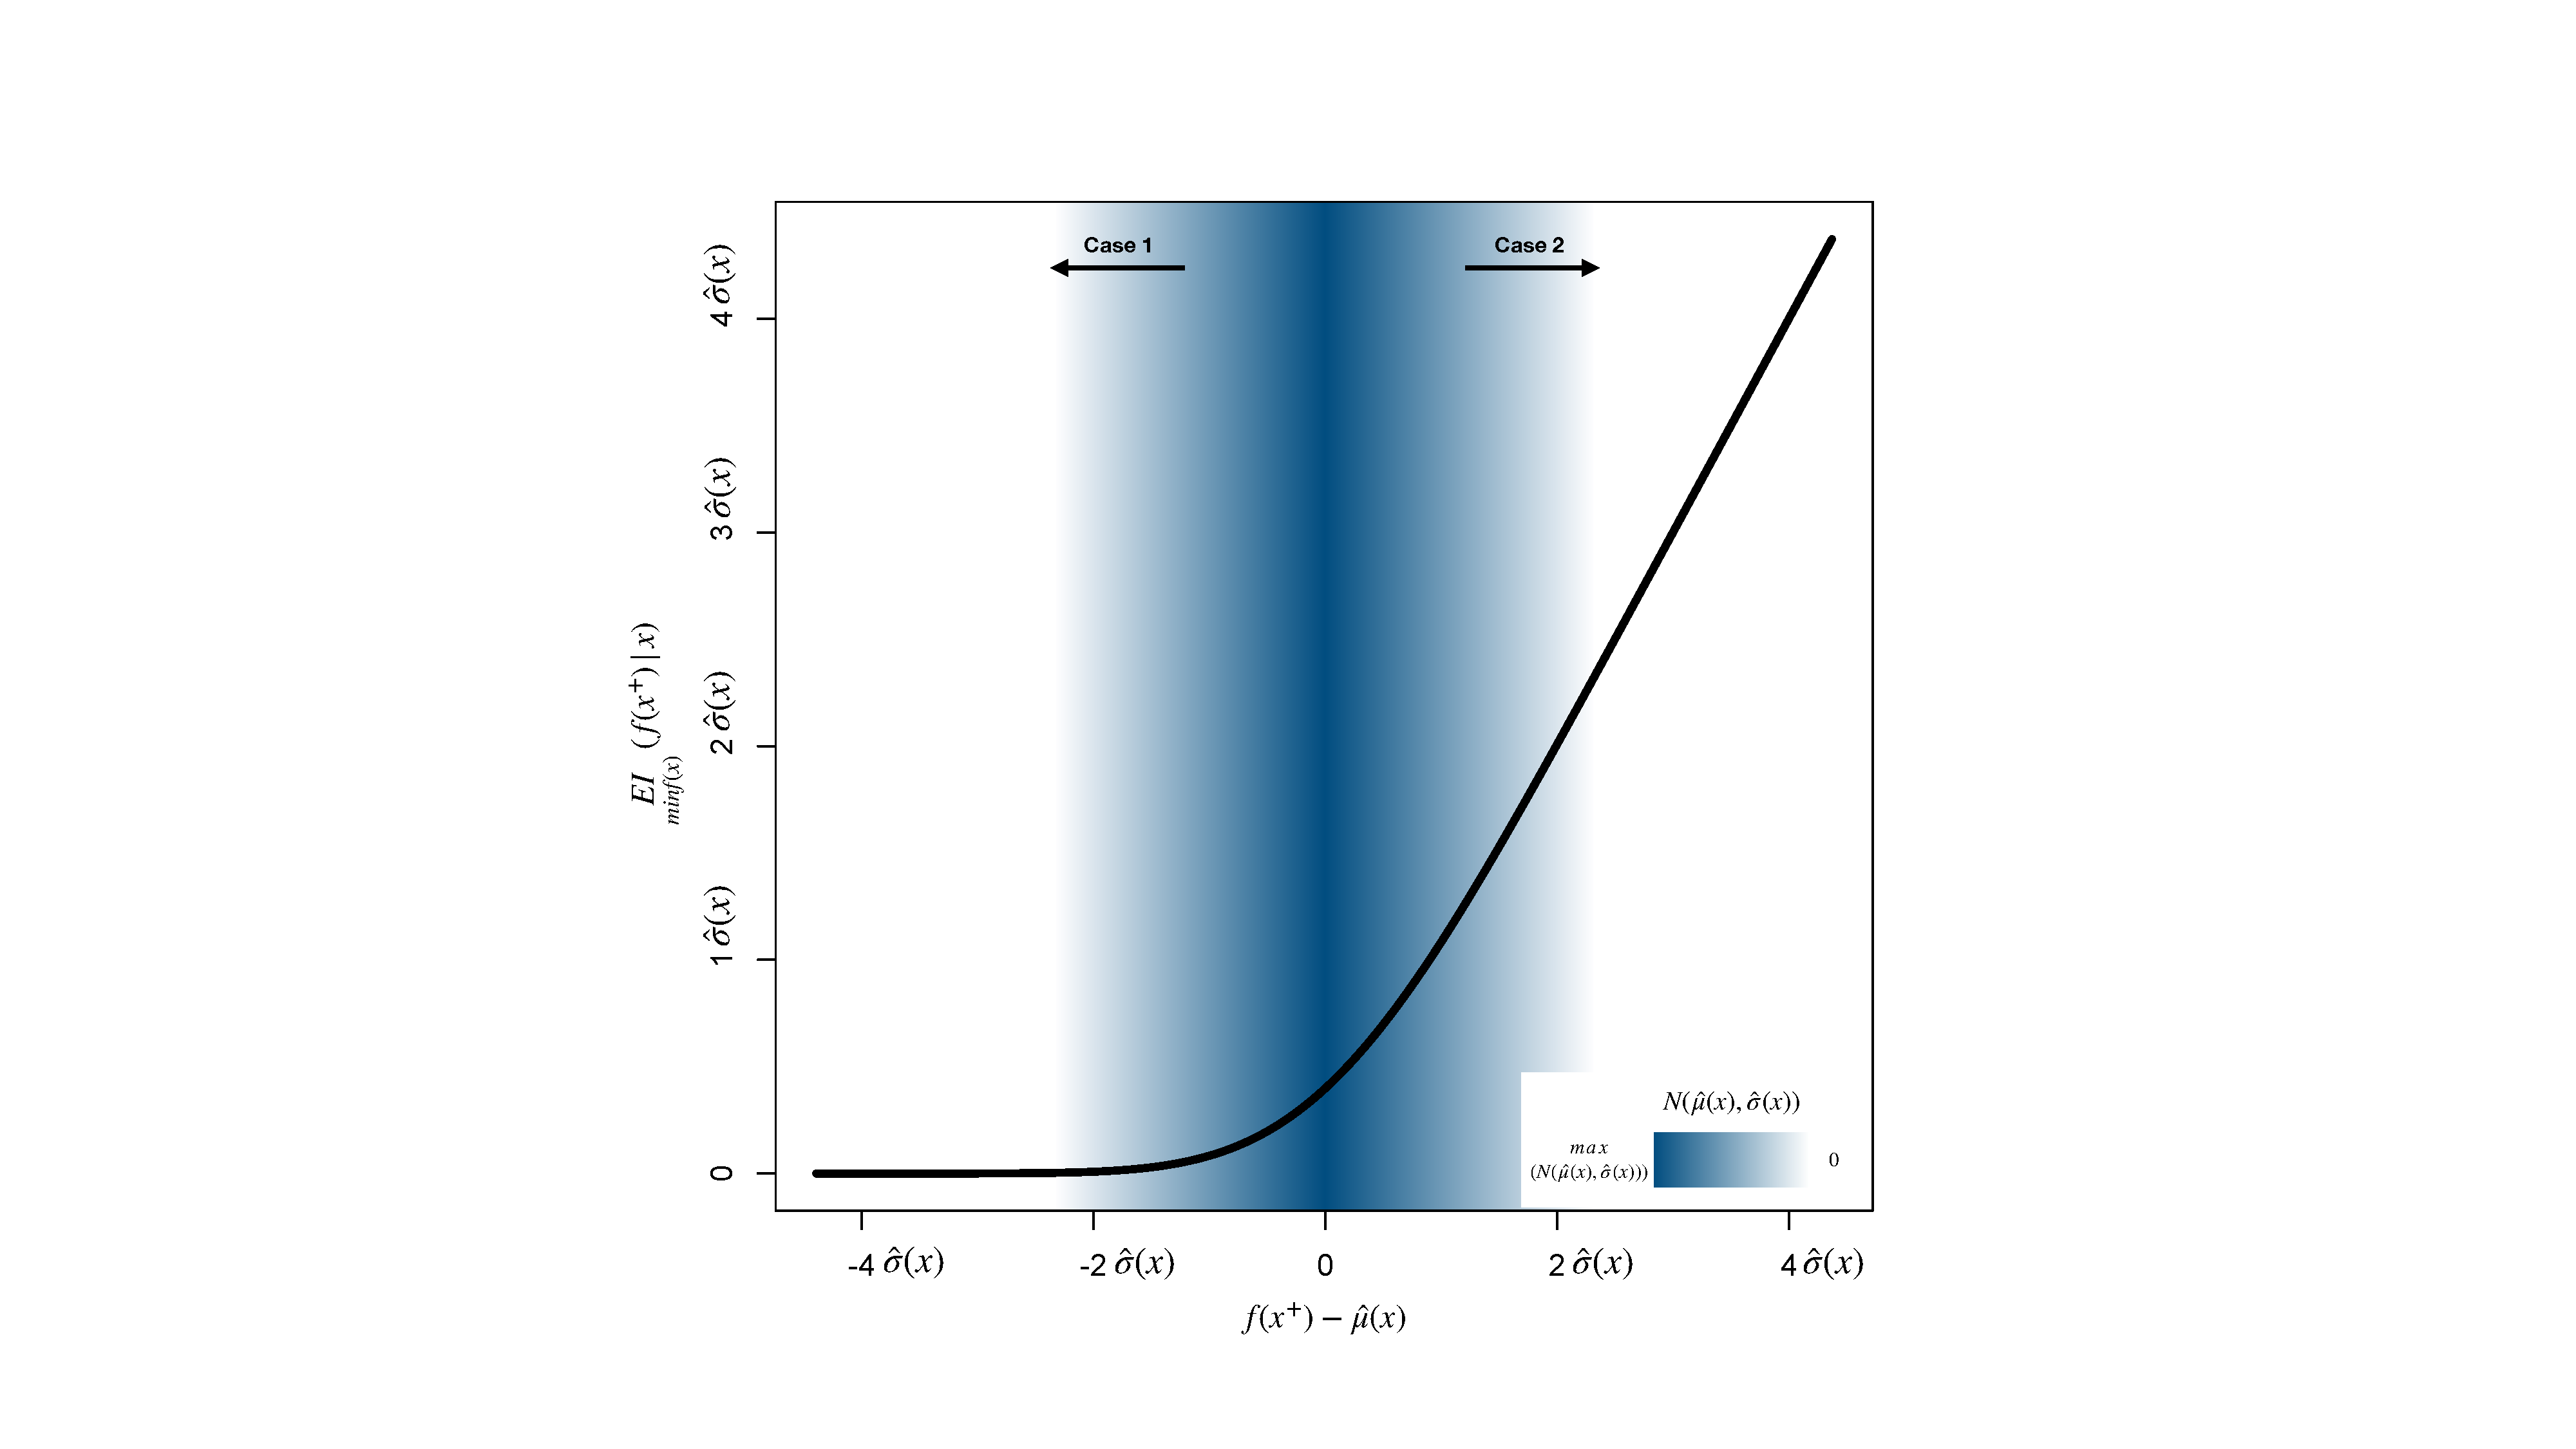
\includegraphics[scale=0.3]{Chapter5/Pictures/Cases_EI.pdf}
    \caption{Variation of $\underset{min f(\bm x)}{EI}(f(\bm x^+)|\bm x)$ for change in reference value $f(\bm x^+)$}
    \label{fig:cases_ei}
\end{figure}

As a first thought, this can be overcome by choosing an appropriate reference value $f_{\mathsf{i}}(\bm x^{\mathsf{i}+})$ depending on the prediction $\hat{f}_{\mathsf{i}}(\bm{x})$. But choosing a reference value $f_{\mathsf{i}}(\bm x^{\mathsf{i}+})$ to define $EI$ depending on where $\hat{f}_{\mathsf{i}}(\bm{x})$ lies in the objective space can make the improvements hard to be compared, since different predictions can have different definition of improvement depending on the choice of the reference value. 
The comparison is also essential for defining NDS for optimization in the context of MOO.
Hence, we augment the $EI$ to have a common frame of reference for comparison, where we consider the axes of the objective space itself as the frame of reference for comparison. The augmentation of $EI$ with $f_{\mathsf{i}}(\bm x^{\mathsf{i}+})$ as reference value is given through the criterion expected value ($EV$)\footnote{We here remind that the expected value can also be otherwise defined as $E(\hat{f}(\bm x))$ in the interval $(-\infty,{f}(\bm x^{++})]$ (detailed in \eqref{EI_cent}) contrary to $EI$ which is defined as $E(f(\bm{x}^{++})-\hat{f}(\bm x))$, but considering $E(\hat{f}(\bm x))$ leads to similar properties as $EI$ in comparing with several reference values} as follows

\begin{equation}
\underset{min f_{\mathsf{i}}(\bm{x})}{EV}(\bm{x}|f_{\mathsf{i}}(\bm x^{\mathsf{i}+})) = f_{\mathsf{i}}(\bm x^{\mathsf{i}+})-\underset{min f_{\mathsf{i}}(\bm{x})}{EI}(\bm{x}| f_{\mathsf{i}}(\bm x^{\mathsf{i}+}))
\label{EV-EI}
\end{equation}

The definition of $EV$ avoids the problem of comparing improvements with several reference values, but the above two cases take a different role for the $EV$ criterion, given as 

\begin{equation}
\begin{array}{l}
\mathbf{Case\,1:}\,
For \,\, \hat{\mu_{\mathsf{i}}}(\bm{x})\pm \hat{\sigma_{\mathsf{i}}}(\bm{x})\gg f_{\mathsf{i}}(\bm x^{\mathsf{i}+}), \, \underset{min f_{\mathsf{i}}(\bm{x})}{EV}(\bm{x}|f_{\mathsf{i}}(\bm x^{\mathsf{i}+}))\approx f_{\mathsf{i}}(\bm x^{\mathsf{i}+})\\
\\
\mathbf{Case\,2:}\,
For \,\, \hat{\mu_{\mathsf{i}}}(\bm{x})\pm \hat{\sigma_{\mathsf{i}}}(\bm{x}) \ll f_{\mathsf{i}}(\bm x^{\mathsf{i}+}), \, \underset{min f_{\mathsf{i}}(\bm{x})}{EV}(\bm{x}|f_{\mathsf{i}}(\bm x^{\mathsf{i}+}))\approx  \hat{\mu_{\mathsf{i}}}(\bm{x})
\end{array}
\end{equation}



For {\textbf{Case 1}}, in the context of $EI$, the improvement becomes infinitesimal or zero for comparison. While in the context of $EV$, this leads to the problem of over-estimation, where the value of $EV$ becomes the reference value itself and hence, an unrealistic reference value can lead to overestimation of improvement. Similarly, the difference in context between $EI$ and $EV$ can be seen for \textbf{Case 2}, where $EV$ simply converges to $\hat{\mu}{(\bm x)}$. This means that two predictions with the same  $\hat{\mu}{(\bm x)}$ but different  $\hat{\sigma_{\mathsf{i}}}(\bm{x})$ will have the same preference. The above cases are graphically shown in Fig. \ref{fig:cases_ev}\\

\begin{figure}[h!]
    \centering
    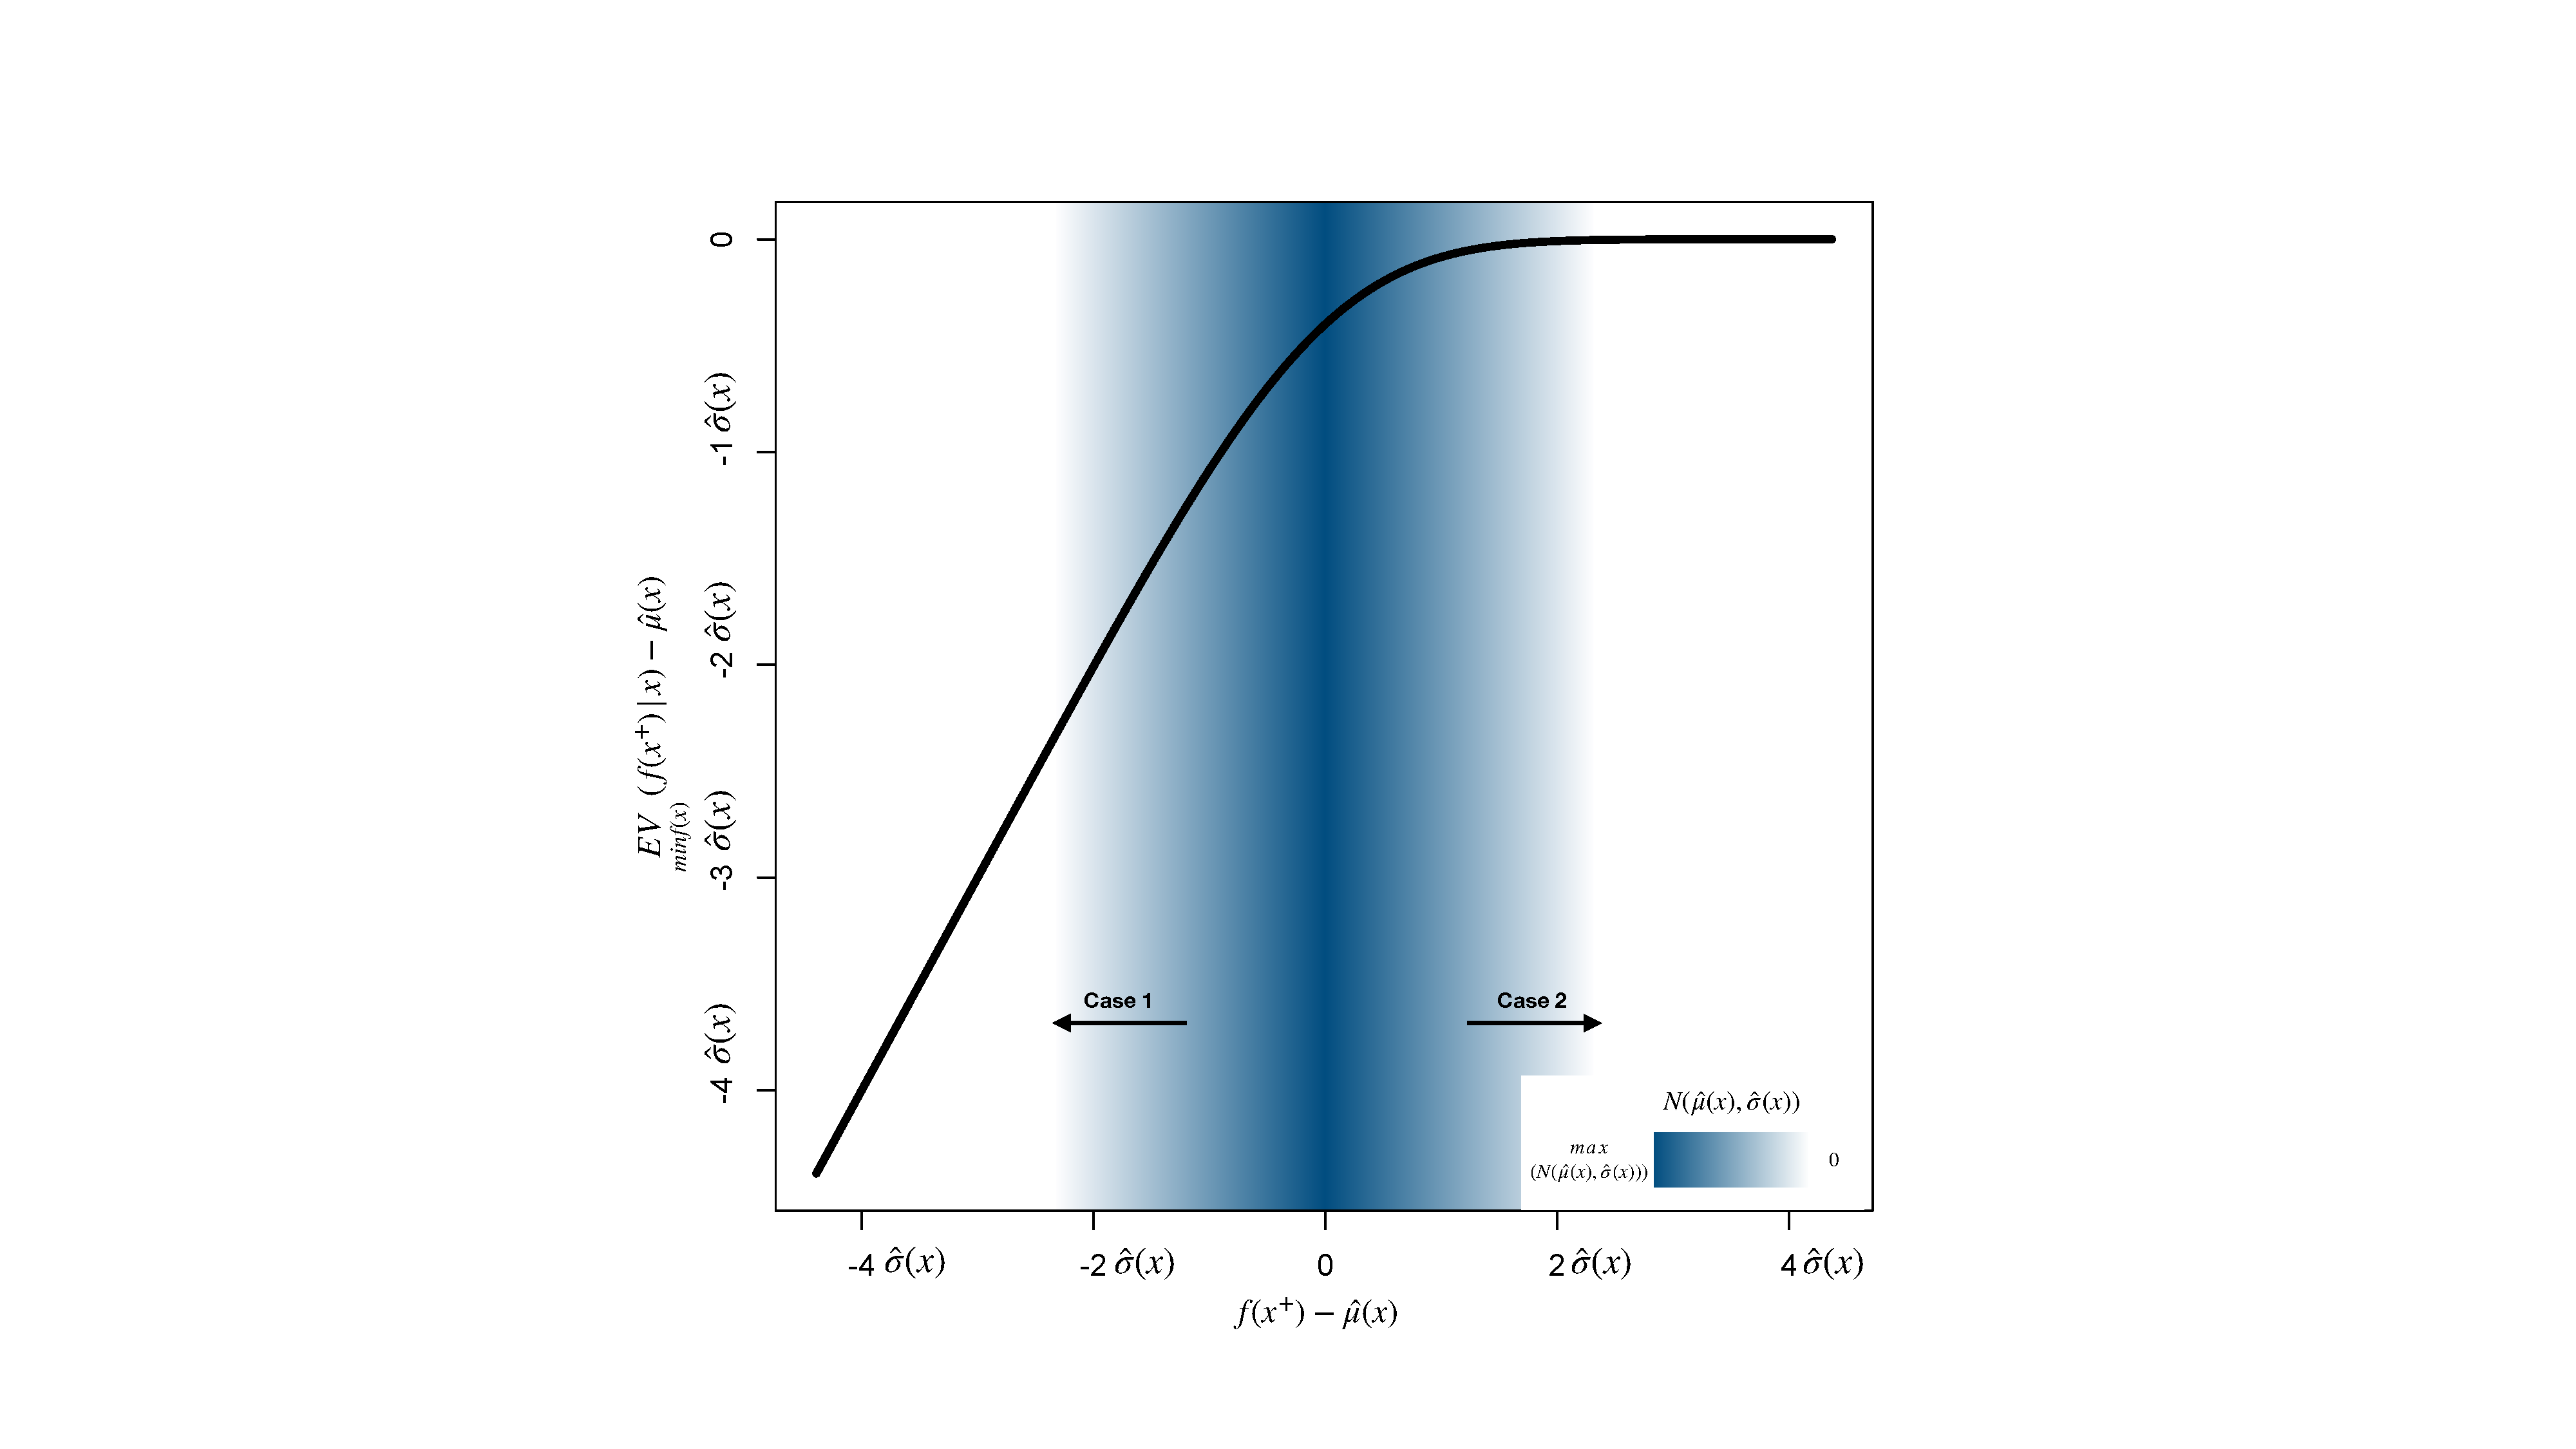
\includegraphics[scale=0.3]{Chapter5/Pictures/Cases_EV.pdf}
    \caption{Variation of $\underset{min f(\bm x)}{EV}(f(\bm x^+)|\bm x)$ for change in reference value $f(\bm x^+)$}
    \label{fig:cases_ev}
\end{figure}

 We give the explanation in avoiding the above cases with $EV$ criterion since it is much easier to work in the coordinates of the objective space. As defined before, \textbf{Case\,1} can be avoided by seeking improvement with respect to a reference value which is more realistic for improvement rather than being too greedy. 
 The realistic scope of improvement considering $f_{\mathsf{i}}(\bm x^{\mathsf{i}+})$ can be defined through the $CDF:$ $\mathcal{P}({f}_{\mathsf{i}}(\bm{x})\leq f_{\mathsf{i}}(\bm x^{\mathsf{i}+}))$ for any $\mathcal{GP}$ outcome $\hat{f}_{\mathsf{i}}(\bm{x}):\mathcal{N}(\hat{\mu_{\mathsf{i}}}(\bm{x}),\hat{\sigma_{\mathsf{i}}}(\bm{x}))$. 
 We here remind that the given $CDF$ is essentially the Probability of Improvement criterion ($PI$). 
 Hence, the $CDF$ constituting to zero for any reference value can be said as being too greedy for improvement, where there can be a limit set for the $CDF$ measure to be considered with compromise on greed. 
 The limit could be set in terms of $\hat{\mu_{\mathsf{i}}}(\bm{x})-\epsilon\hat{\sigma_{\mathsf{i}}}(\bm{x})$\footnote{We give the relation in terms of $LCB$, since for any $f(\bm x^{+}):\mathcal{P}({f}(\bm{x})\leq f(\bm x^{+}))\geq\mathcal{P}({f}(\bm{x})\leq \hat{\mu}(\bm{x})-\epsilon\hat{\sigma}(\bm{x}))$, the following relation holds $f(\bm x^{+}) \geq \hat{\mu}(\bm{x})-\epsilon\hat{\sigma}(\bm{x})$ } where we seek for $\mathcal{P}({f}_{\mathsf{i}}(\bm{x})\leq f_{\mathsf{i}}(\bm x^{\mathsf{i}+}))\geq\mathcal{P}({f}_{\mathsf{i}}(\bm{x})\leq \hat{\mu_{\mathsf{i}}}(\bm{x})-\epsilon\hat{\sigma_{\mathsf{i}}}(\bm{x}))$, with $\epsilon$ being the parameter to be defined. 
 A higher value of $\epsilon$ means higher the greed to seek improvement, but the balance to set the limit could be otherwise seen as the acceptable risk that can be considered for exploration. The higher risk with considering higher value of $\epsilon$ for $\hat{\mu_{\mathsf{i}}}(\bm{x})-\epsilon\hat{\sigma_{\mathsf{i}}}(\bm{x})$ may reap higher benefits but this could be otherwise, since there is equal probability for ${f}_{\mathsf{i}}(\bm{x})\geq\hat{\mu_{\mathsf{i}}}(\bm{x})+\epsilon\hat{\sigma_{\mathsf{i}}}(\bm{x})$. Hence, this requires the right balance for the choice of $\epsilon$ with acceptable risk for exploration.\\

For MOO, the most feasible improvement that we can look for is with respect to the empirical Pareto-front $f_{\mathsf{i}}(\mathscr{P}_{\mathcal{S}}):=\{f_{\mathsf{i}}(\bm{p}_1),f_{\mathsf{i}}(\bm{p}_2),\hdots,f_{\mathsf{i}}(\bm{p}_{(.)})\}$ of the observed samples. But, there can be multiple $\bm{p}_{\mathrm i}:f_{\mathsf i}(\bm{p}_{\mathrm{i}})\leq\hat{\mu_{\mathsf{i}}}(\bm{x})-\epsilon\hat{\sigma_{\mathsf{i}}}(\bm{x})$, where we choose the $\bm{p}_\mathrm{i}$ which gives the minimum value of $\underset{min f_{\mathsf{i}}(\bm{x})}{EV}$. The choice of the minimum value of $\underset{min f_{\mathsf{i}}(\bm{x})}{EV}$ for a function to be minimised averts \textbf{Case\,2} which defines the pessimistic choice of reference value, unless it is not possible when no suitable reference value exists. In overall, the above definitions provide the balance between greed and being pessimistic for improvement through the parameter $\epsilon$. The above definitions could be expressed as follows

\begin{equation} \label{EV_f}
\begin{split}
\underset{min\,f_{\mathsf{i}}(\bm{x})}{EV}(\bm{x}|\mathscr{P}_{\mathcal{S}},\epsilon) &= \underset{\bm{p}_{\mathrm i}\in \mathscr{P}_s}{min}(\underset{min f_{\mathsf{i}}(\bm{x})}{EV}(f_{\mathsf{i}}(\bm{p}_{\mathrm{i}})|\bm{x})) \\
\mathscr{P}_s &:=\{  f_{\mathsf{i}}(\bm{p}_{\mathrm i})\geq\hat{\mu_{\mathsf{i}}}(\bm{x})-\epsilon\hat{\sigma_{\mathsf{i}}}(\bm{x}),\forall\bm{p}_{\mathrm i}\in\mathscr{P}_{\mathcal{S}}\}
\end{split}
\end{equation}

where the discrete optimisation of $\underset{\bm{p}_{\mathrm i}\in \mathscr{P}_s}{min}(\underset{min f_{\mathsf{i}}(\bm{x})}{EV}(f_{\mathsf{i}}(\bm{p}_{\mathrm i})|\bm{x}))$ can be implicitly satisfied through defining NDS with $\underset{min\,f_{\mathsf{i}}(\bm{x})}{EV}(\bm{x}|\mathscr{P}_{\mathcal{S}},\epsilon)$. 
Alternatively, from the nature of proportionality for $\underset{min f_{\mathsf{i}}(\bm{x})}{EV}(f_{\mathsf{i}}(\bm{p}_{\mathrm{i}})|\bm{x})) \propto f_{\mathsf{i}}(\bm{p}_{\mathrm i})$, shown in Fig. \ref{fig:cases_ev}, the most suitable reference value $f_{\mathsf{i}}(\bm{p}_{\mathrm i}^\star)$ to achieve $\underset{\bm{p}_{\mathrm i} \in \mathscr{P}_s}{min}(\underset{min f_{\mathsf{i}}(\bm{x})}{EV}(f_{\mathsf{i}}(\bm{p}_{\mathrm i})|\bm{x}))$ can be simply given as  $f(\bm{p}_{\mathrm i}^\star)=\underset{\bm{p}_{\mathrm i}\in \mathscr{P}_s}{min} f(\bm{p}_{\mathrm i})$.  In short, we define the Eq. \eqref{EV_f} as $EV$ criterion for the following discussions.\\

The given definitions allow to define $EV$ criterion in the place of $EI$, where the problem \eqref{Optim_EIs} can be redefined as follows

 \begin{equation}\label{Optim_EVs}
 \underset{\bm x \in \mathcal{X}}{min}\Big[ \underset{min\,f_1(\bm{x})}{EV}(\bm{x}|\mathscr{P}_{\mathcal{S}},\epsilon) \cdots \underset{min\,f_{\mathsf{m}}(\bm{x})}{EV}(\bm{x}|\mathscr{P}_{\mathcal{S}},\epsilon)  \Big]
 \end{equation}
 
 The MOO can be achieved through NSGA-2, which leads to Pareto-optimal solutions $(\mathscr{P}_{\hat{\mathcal{S}}})$. The independent definition of improvement allows to work with only univariate Gaussian distributions and hence, large number of $EV$ criteria could be optimised with relatively ease.\\
 
 The primary goal for choosing $f_{\mathsf{i}}(\bm{p}_{\mathrm i}) \in f_{\mathsf{i}}(\mathscr{P}_{\mathcal{S}})$ independently for each $\underset{min\,f_{\mathsf{i}}(\bm{x})}{EV}(\bm{x}|\mathscr{P}_{\mathcal{S}},\epsilon)$ is that it can lead to choosing reference points $\bm f(\bm{p}_{\mathrm i}) \in \bm f(\mathscr{P}_{\mathcal{S}})$, where the intention is to define improvements $\mathfrak{I}_{\bm f(\bm{p}_{\mathrm i})}$ 
 %\footnote{$\mathscr{I}_{\bm{f}^*} (\bm x) =\Big[\underset{min\,f_1(\bm{x})}{EV}(\bm x|f^*_1) \cdots \underset{min\,f_{\mathsf{m}}(\bm{x})}{EV}(\bm x|f^*_{\mathsf{m}})\Big]$, {\bm{f}^* =[f^*_1 \cdots f^*_{\mathsf{m}}]} }
  \footnote{$\mathscr{I}_{\bm{f}^*} (\bm x)$ $\in \mathfrak{I}_{\bm{f}^*}=$$\Big\{\Big[\underset{min\,f_1(\bm{x})}{EV}(\bm x|f^*_1) \cdots \underset{min\,f_{\mathsf{m}}(\bm{x})}{EV}(\bm x|f^*_{\mathsf{m}})\Big]| \forall \mathsf{i},f_{\mathsf{i}}^{*} = \underset{\bm{p}_{\mathrm i}\in \mathscr{P}_s}{min} f_{\mathsf{i}}(\bm{p}_{\mathrm i}), \forall \bm x \in \mathcal{X}\Big\}$, ${\bm{f}^* =[f^*_1 \cdots f^*_{\mathsf{m}}]}$} (Fig. \ref{fig:improv_illus}). %where $\mathfrak{I}_{\bm{f}^*}$ is the set of all possible improvements with respect to the reference point $\bm{f}^*$} that can dominate $\bm f(\bm{p}_{\mathrm i}) \in  \bm f(\mathscr{P}_{\mathcal{S}})$.
 The choice of $f_{\mathsf{i}}(\bm{p}_{\mathrm i})$ independently for each $\underset{min\,f_{\mathsf{i}}(\bm{x})}{EV}(\bm{x}|\mathscr{P}_{\mathcal{S}},\epsilon)$ means that it can implicitly lead to choosing reference points $[\bm g_{\mathsf 1}= f_{\mathsf{1}}(\bm{p}_{\mathrm i}) \in f_{\mathsf{1}}(\mathscr{P}_{\mathcal{S}}), \cdots, \bm g_{\mathsf m}= f_{\mathsf{m}}(\bm{p}_{\mathrm i}) \in f_{\mathsf{m}}(\mathscr{P}_{\mathcal{S}}) ]$\footnote{It should be noted that the choice of $\bm{p}_{\mathrm i}$ is independent for each $f_{\mathsf{i}}$}$\in \mathbb{R}^{\mathsf{m}}$ from a grid of points $\mathscr{G}:=\{f_{\mathsf{1}}(\mathscr{P}_{\mathcal{S}}) \times \cdots  \times f_{\mathsf{m}}(\mathscr{P}_{\mathcal{S}})\}$. 
This means that $\bm f(\mathscr{P}_{\mathcal{S}})\subset\mathscr{G}$, where $\mathscr{G}$ also contains points which dominate or be dominated by points in the set $\bm f(\mathscr{P}_{\mathcal{S}})$, which includes the Utopian point: $\bm g_{\mathsf{o}} \preceq \bm f(\mathscr{P}_{\mathcal{S}})$ \footnote{$\bm g_{\mathsf o} $ is an arbitrary point in $\mathscr{G}$ with index $\mathsf{o}$} and the Nadir point: $\forall {\mathrm{i}}, \bm f(\bm p_{\mathrm{i}})  \preceq {\bm g_{\mathsf{o}}}$.  
  \iffalse
  This means that any improvement $ \mathscr{I}_{\bm {g}_{\mathsf o}}$ defined with a reference point $\bm {g}_{\mathsf j} \in \mathscr{G}$ falls in to one of the categories, 
  
  \begin{itemize}
  \item if $\bm g_{\mathsf{o}} \in \bm f(\mathscr{P})$, then $\mathscr{I}_{f_{\mathsf{i}}(\bm{p}_{\mathrm i})}$ can be said to dominate a point $\bm f(\bm p_{\mathrm{i}})$ in the Pareto-front,  where $\bm f(\bm p_{\mathrm{i}}) = \bm g_{\mathsf{j}}$
  \item if $\bm g_{\mathsf{j}} \preceq \bm f(\bm p_{\mathrm{i}})$, then any improvement defined with $\bm g_{\mathsf{j}}$ also dominates $f(\bm p_{\mathrm{i}})$ 
   \item if $\bm f(\bm p_{\mathrm{i}}) \preceq \bm g_{\mathsf{j}}$

  \end{itemize}
  \fi
  This means that improvements can not only be defined to dominate any empirical Pareto-front point $\bm f({\bm{p}_{\mathrm{i}}}) \in \bm f  (\mathscr{P}_{\mathcal{S}})$, but also multiple Pareto-front points in the set $\bm f(\mathscr{P}_{\mathcal{S}})$.\\
  
  \begin{figure}
     \centering
    \includegraphics[scale=0.35]{Chapter5/Pictures/improv_illus}
    \caption{Illustration of the set $\mathfrak{I}_{\bm f(\bm{p}_{\mathrm i})}$ and its associated subsets}
    \label{fig:improv_illus}
 \end{figure}
  
 With the population based evolutionary strategy of NSGA-2, for a given population, the optimisation is simultaneously defined with several reference points in the objective space. This means that the individuals in a given generation of NSGA-2 are defined with their respective reference point and since the improvements are represented as expected values in the objective space, comparisons can be made to define non-dominated sorting and niching operations. This implicitly models optimisation of several $EI$s in the objective space, with each $EI$ defined with a unique reference point, illustrated in \ref{fig:EV_EIss}. \\
  
  
 
 
  %Though, a reference value $f_{\mathsf{i}}(\bm{p}_{\mathrm i}) \in f_{\mathsf{i}}(\mathscr{P}_{\mathcal{S}})$ is chosen independently for each $\underset{min\,f_{\mathsf{i}}(\bm{x})}{EV}(\bm{x}|\mathscr{P}_{\mathcal{S}},\epsilon)$, this implicitly leads to choosing a reference point $[f_{\mathsf{1}}(\bm{p}_{\mathrm i}) \in f_{\mathsf{1}}(\mathscr{P}_{\mathcal{S}}), \cdots, f_{\mathsf{m}}(\bm{p}_{\mathrm i}) \in f_{\mathsf{m}}(\mathscr{P}_{\mathcal{S}}) ]$\footnote{It should be noted that the choice of $\bm{p}_{\mathrm i}$ is independent for each $f_{\mathsf{i}}$}$\in \mathbb{R}^{\mathsf{m}}$from a grid of points $\{f_{\mathsf{1}}(\mathscr{P}_{\mathcal{S}}) \times f_{\mathsf{2}}(\mathscr{P}_{\mathcal{S}})  \times \cdots  \times f_{\mathsf{m}}(\mathscr{P}_{\mathcal{S}})\}$ for any prediction $\bm{\hat{f}}(\bm x)$. 
  %For $\mathsf{n}_{\mathscr{P}_{{\mathcal{S}}}}$ number of points in $\mathscr{P}_{\mathcal{S}}$, number of grid points scale by  ${(\mathsf{n}_{\mathscr{P}_{{\mathcal{S}}}}})^\mathsf{m}$. This can be seen as improvement being defined independently with each reference point in $\mathbb{R}^{\mathsf{m}}$, where the improvement defines the dominance in $\mathbb{R}^{\mathsf{m}}$ over its respective reference point.
 %Hence, the optimisation of the improvement is also simultaneously defined with several reference points in the objective space. This means that the individuals in a given generation of NSGA-2 are defined with their respective reference point and since the improvements are represented as the expected values in the objective space, comparisons can be made to define non-dominated sorting and niching operations.\\
 
 \begin{figure}
     \centering
    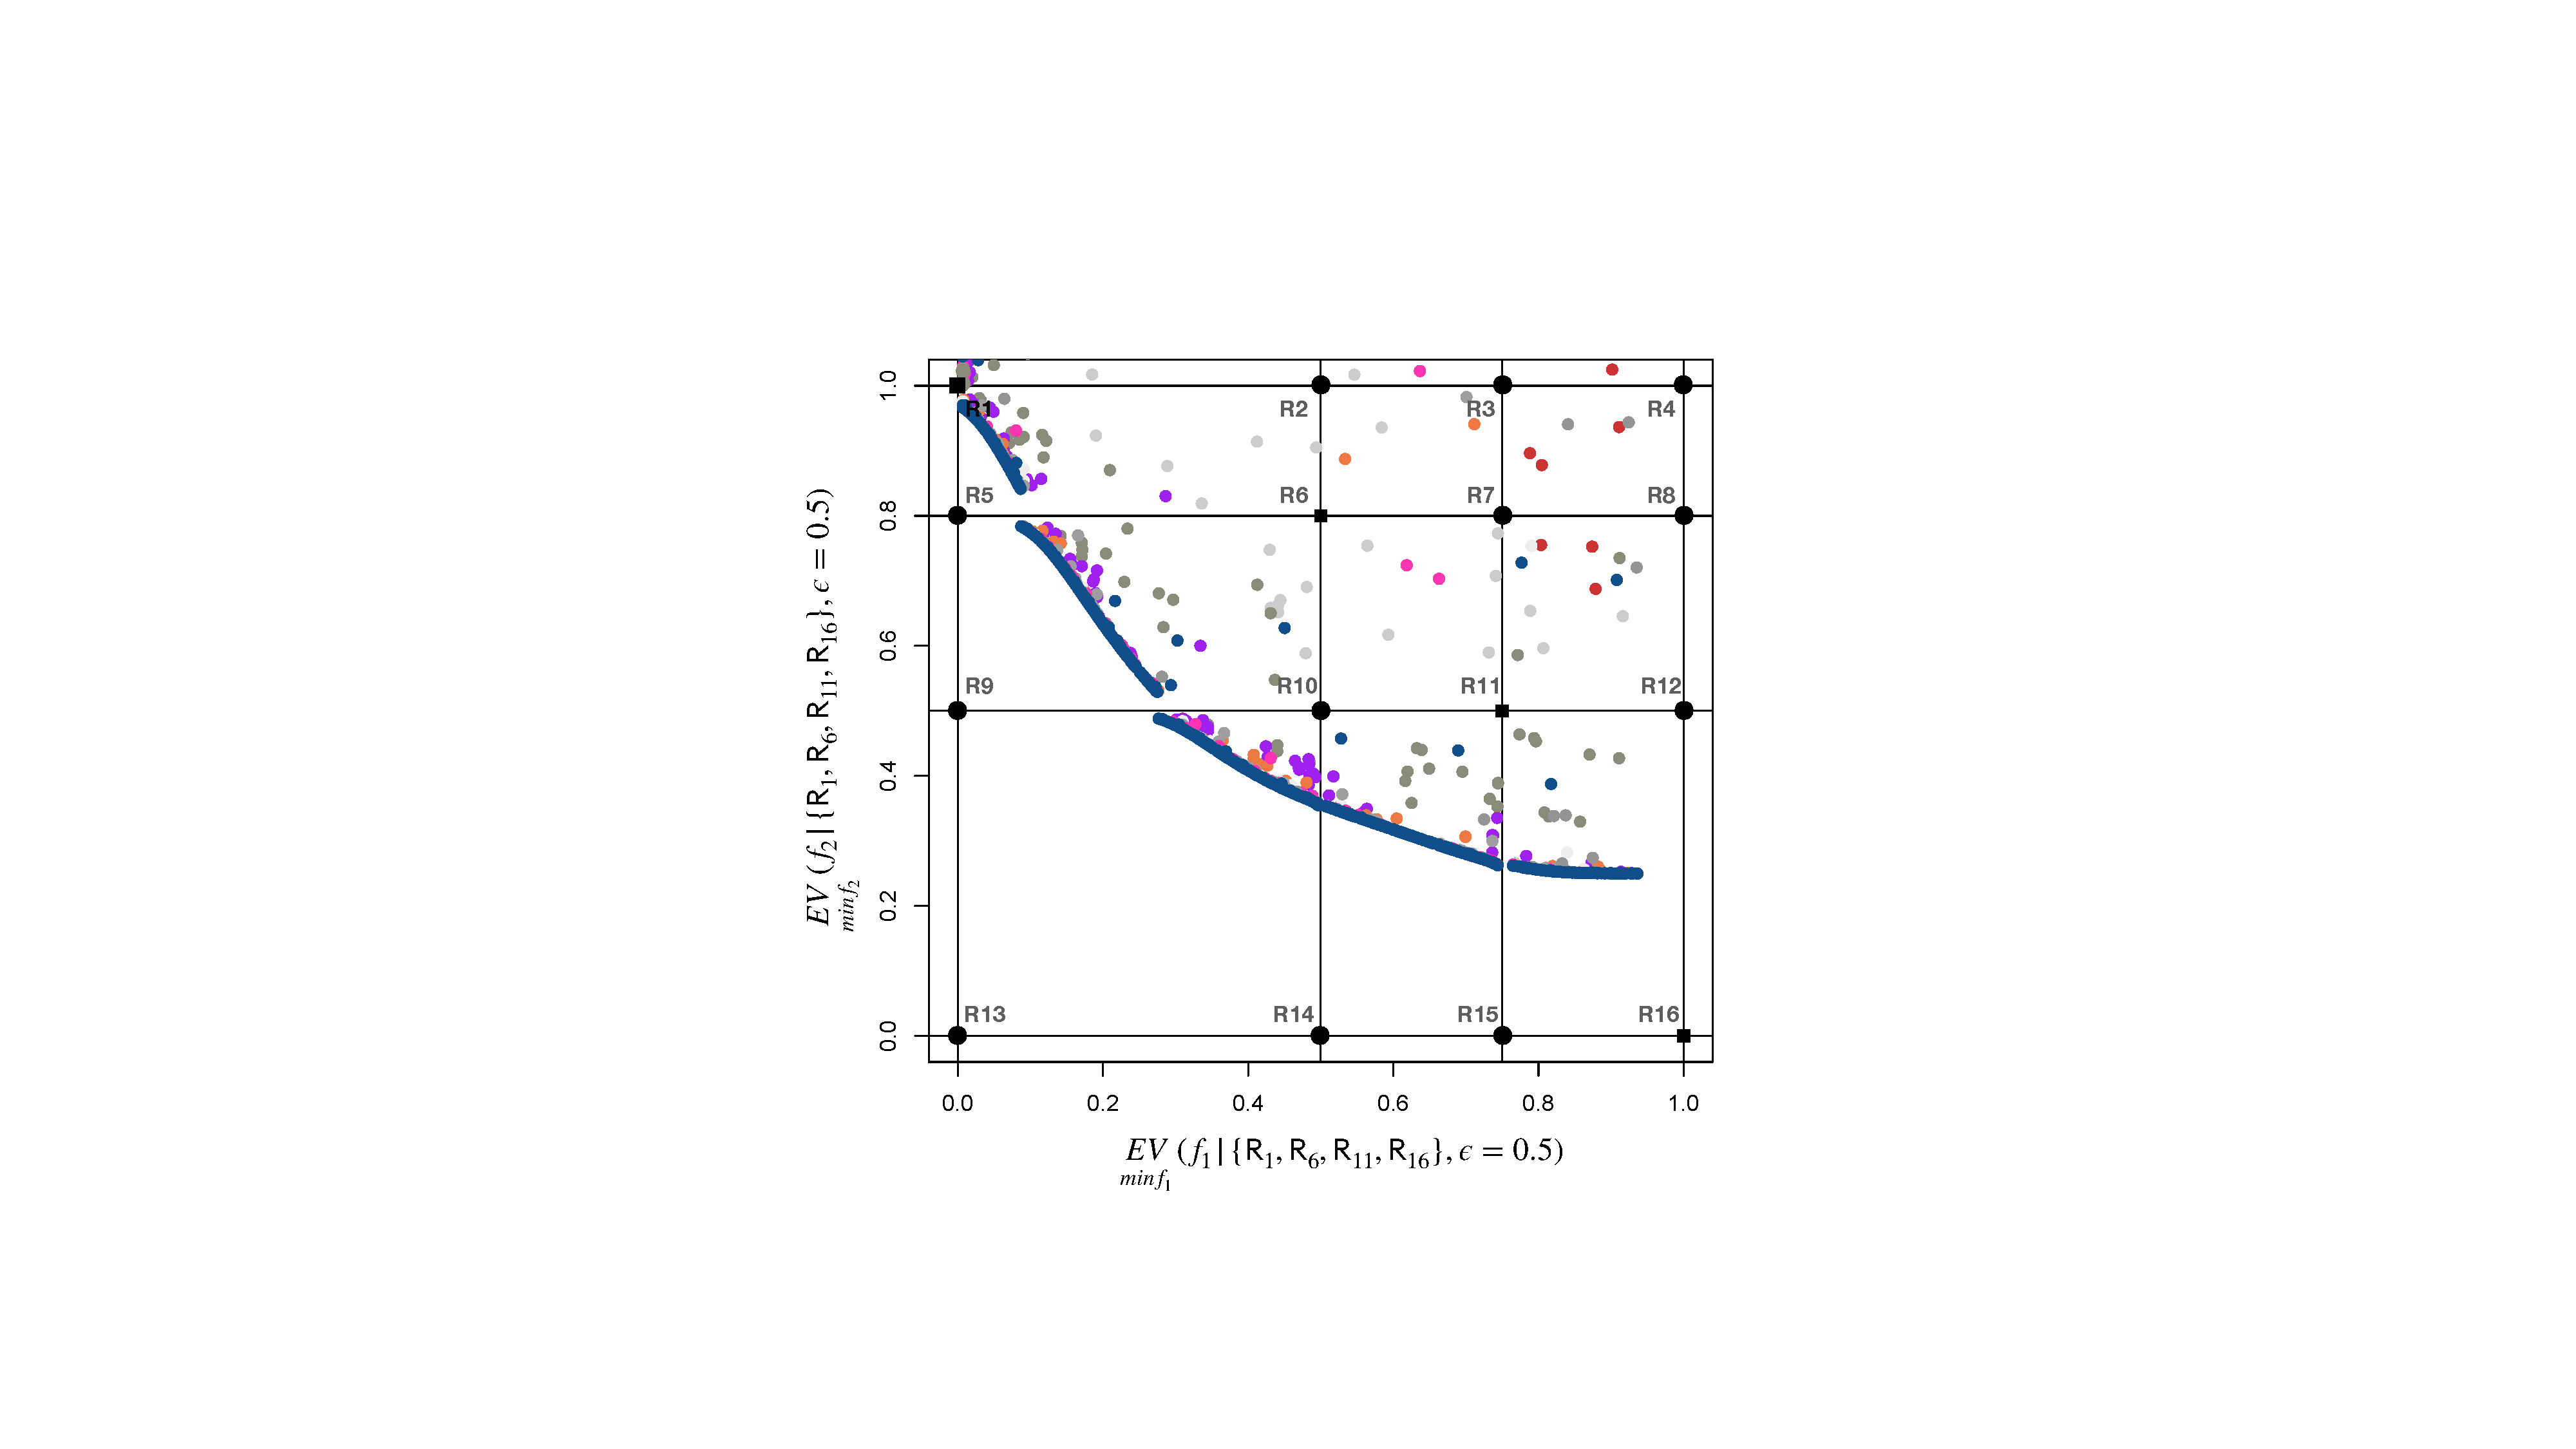
\includegraphics[scale=0.4]{Chapter5/Pictures/EV_ZDT1.pdf}
    \caption{An example for optimization of EV}
    \label{fig:eg:EV}
 \end{figure}
 
 An example for the optimisation of \eqref{Optim_EVs} is shown in Fig. , for a simple MOO test functions set: ZDT1 of two dimensions $(\mathsf{m}=2)$. 
 In this case, $\bm f(\mathscr{P}_{\mathcal{S}})=\{\bm{\mathsf{R}}_1, \bm{\mathsf{R}}_6, \bm{\mathsf{R}}_{11}, \bm{\mathsf{R}}_{16}\}$, $\mathscr{G}=\{\bm{\mathsf{R}}_1,\cdots,\bm{\mathsf{R}}_{16}\}$.
The Pareto front  $\bm f(\mathscr{P}_{\hat{\mathcal{S}}})$ is defined by the reference points $\bm{\mathsf{R}}_{2},\bm{\mathsf{R}}_{6},\bm{\mathsf{R}}_{10},\bm{\mathsf{R}}_{11},\bm{\mathsf{R}}_{16}$, where two of the reference points $\bm{\mathsf{R}}_6$ and $\bm{\mathsf{R}}_{11}$ belong to $\mathscr{P}_{\mathcal{S}}$. This means that the improvements $\mathfrak{I}_{\bm{\mathsf{R}}_6}$ and $\mathfrak{I}_{\bm{\mathsf{R}}_{11}}$ independently define domination over $\bm{\mathsf{R}}_6$ and $\bm{\mathsf{R}}_{11}$ respectively, as $\mathfrak{I}_{\bm{\mathsf{R}}_6} \preceq \bm{\mathsf{R}}_6$ and $\mathfrak{I}_{\bm{\mathsf{R}}_{11}} \preceq \bm{\mathsf{R}}_{11}$.
For $\bm{\mathsf{R}}_{10}$, something interesting happens, where $\bm{\mathsf{R}}_{10} \notin \mathscr{P}_{\mathcal{S}}$ but is purely an outcome of the implicit definition of grid $\mathscr{G}$. In this case, $\bm{\mathsf{R}}_{10} \preceq \{\bm{\mathsf{R}}_6$,  $\bm{\mathsf{R}}_{11}\}$, hence also the improvements $\mathfrak{I}_{\bm{\mathsf{R}}_{10}} \preceq \{\bm{\mathsf{R}}_6$,  $\bm{\mathsf{R}}_{11}\}$, i.e., any improvement $\mathscr{I}_{\bm{\mathsf{R}}_{10}} \in \mathfrak{I}_{\bm{\mathsf{R}}_{10}}$ dominates the two Pareto-front points $\bm{\mathsf{R}}_6$ and $\bm{\mathsf{R}}_{11}$. 
Hence, $\mathscr{G}$ consists of reference points to define improvements with respect to any $\bm f (\bm p_{\mathrm i})$ or combination of several $\bm f (\bm p_{\mathrm i})$. $\mathscr{G}$ also contains points $\bm g_{\mathsf{o}}: \bm f(\mathscr{P}_{\mathcal{S}})\preceq \bm g_{\mathsf{o}}$ where the improvements defined with such points are essential for guiding the solutions to define $\mathscr{P}_{\hat{\mathcal{S}}}$. The reference points $\bm{\mathsf{R}}_2$ and $\bm{\mathsf{R}}_{12}$ are also weakly dominated by the points in the set $\bm f(\mathscr{P}_{\mathcal{S}})$, where in this case, the improvements $\mathfrak{I}_{\bm{\mathsf{R}}_2}$ are presumed to define the intermediate points between ${\bm{\mathsf{R}}_1}$ and ${\bm{\mathsf{R}}_6}$, and similarly the improvements $\mathfrak{I}_{\bm{\mathsf{R}}_{12}}$ are presumed to define the intermediate points between ${\bm{\mathsf{R}}_{11}}$ and ${\bm{\mathsf{R}}_{16}}$.
In this example, the Utopian point corresponds to ${\bm{\mathsf{R}}_{12}} \preceq \bm f(\mathscr{P}_{\mathcal{S}})$ and the Nadir point corresponds to  ${\bm{\mathsf{R}}_4}$ where all the points in $\mathscr{G}$ except ${\bm{\mathsf{R}}_4}$ dominates ${\bm{\mathsf{R}}_4}$. \\


 \begin{figure}
     \centering
    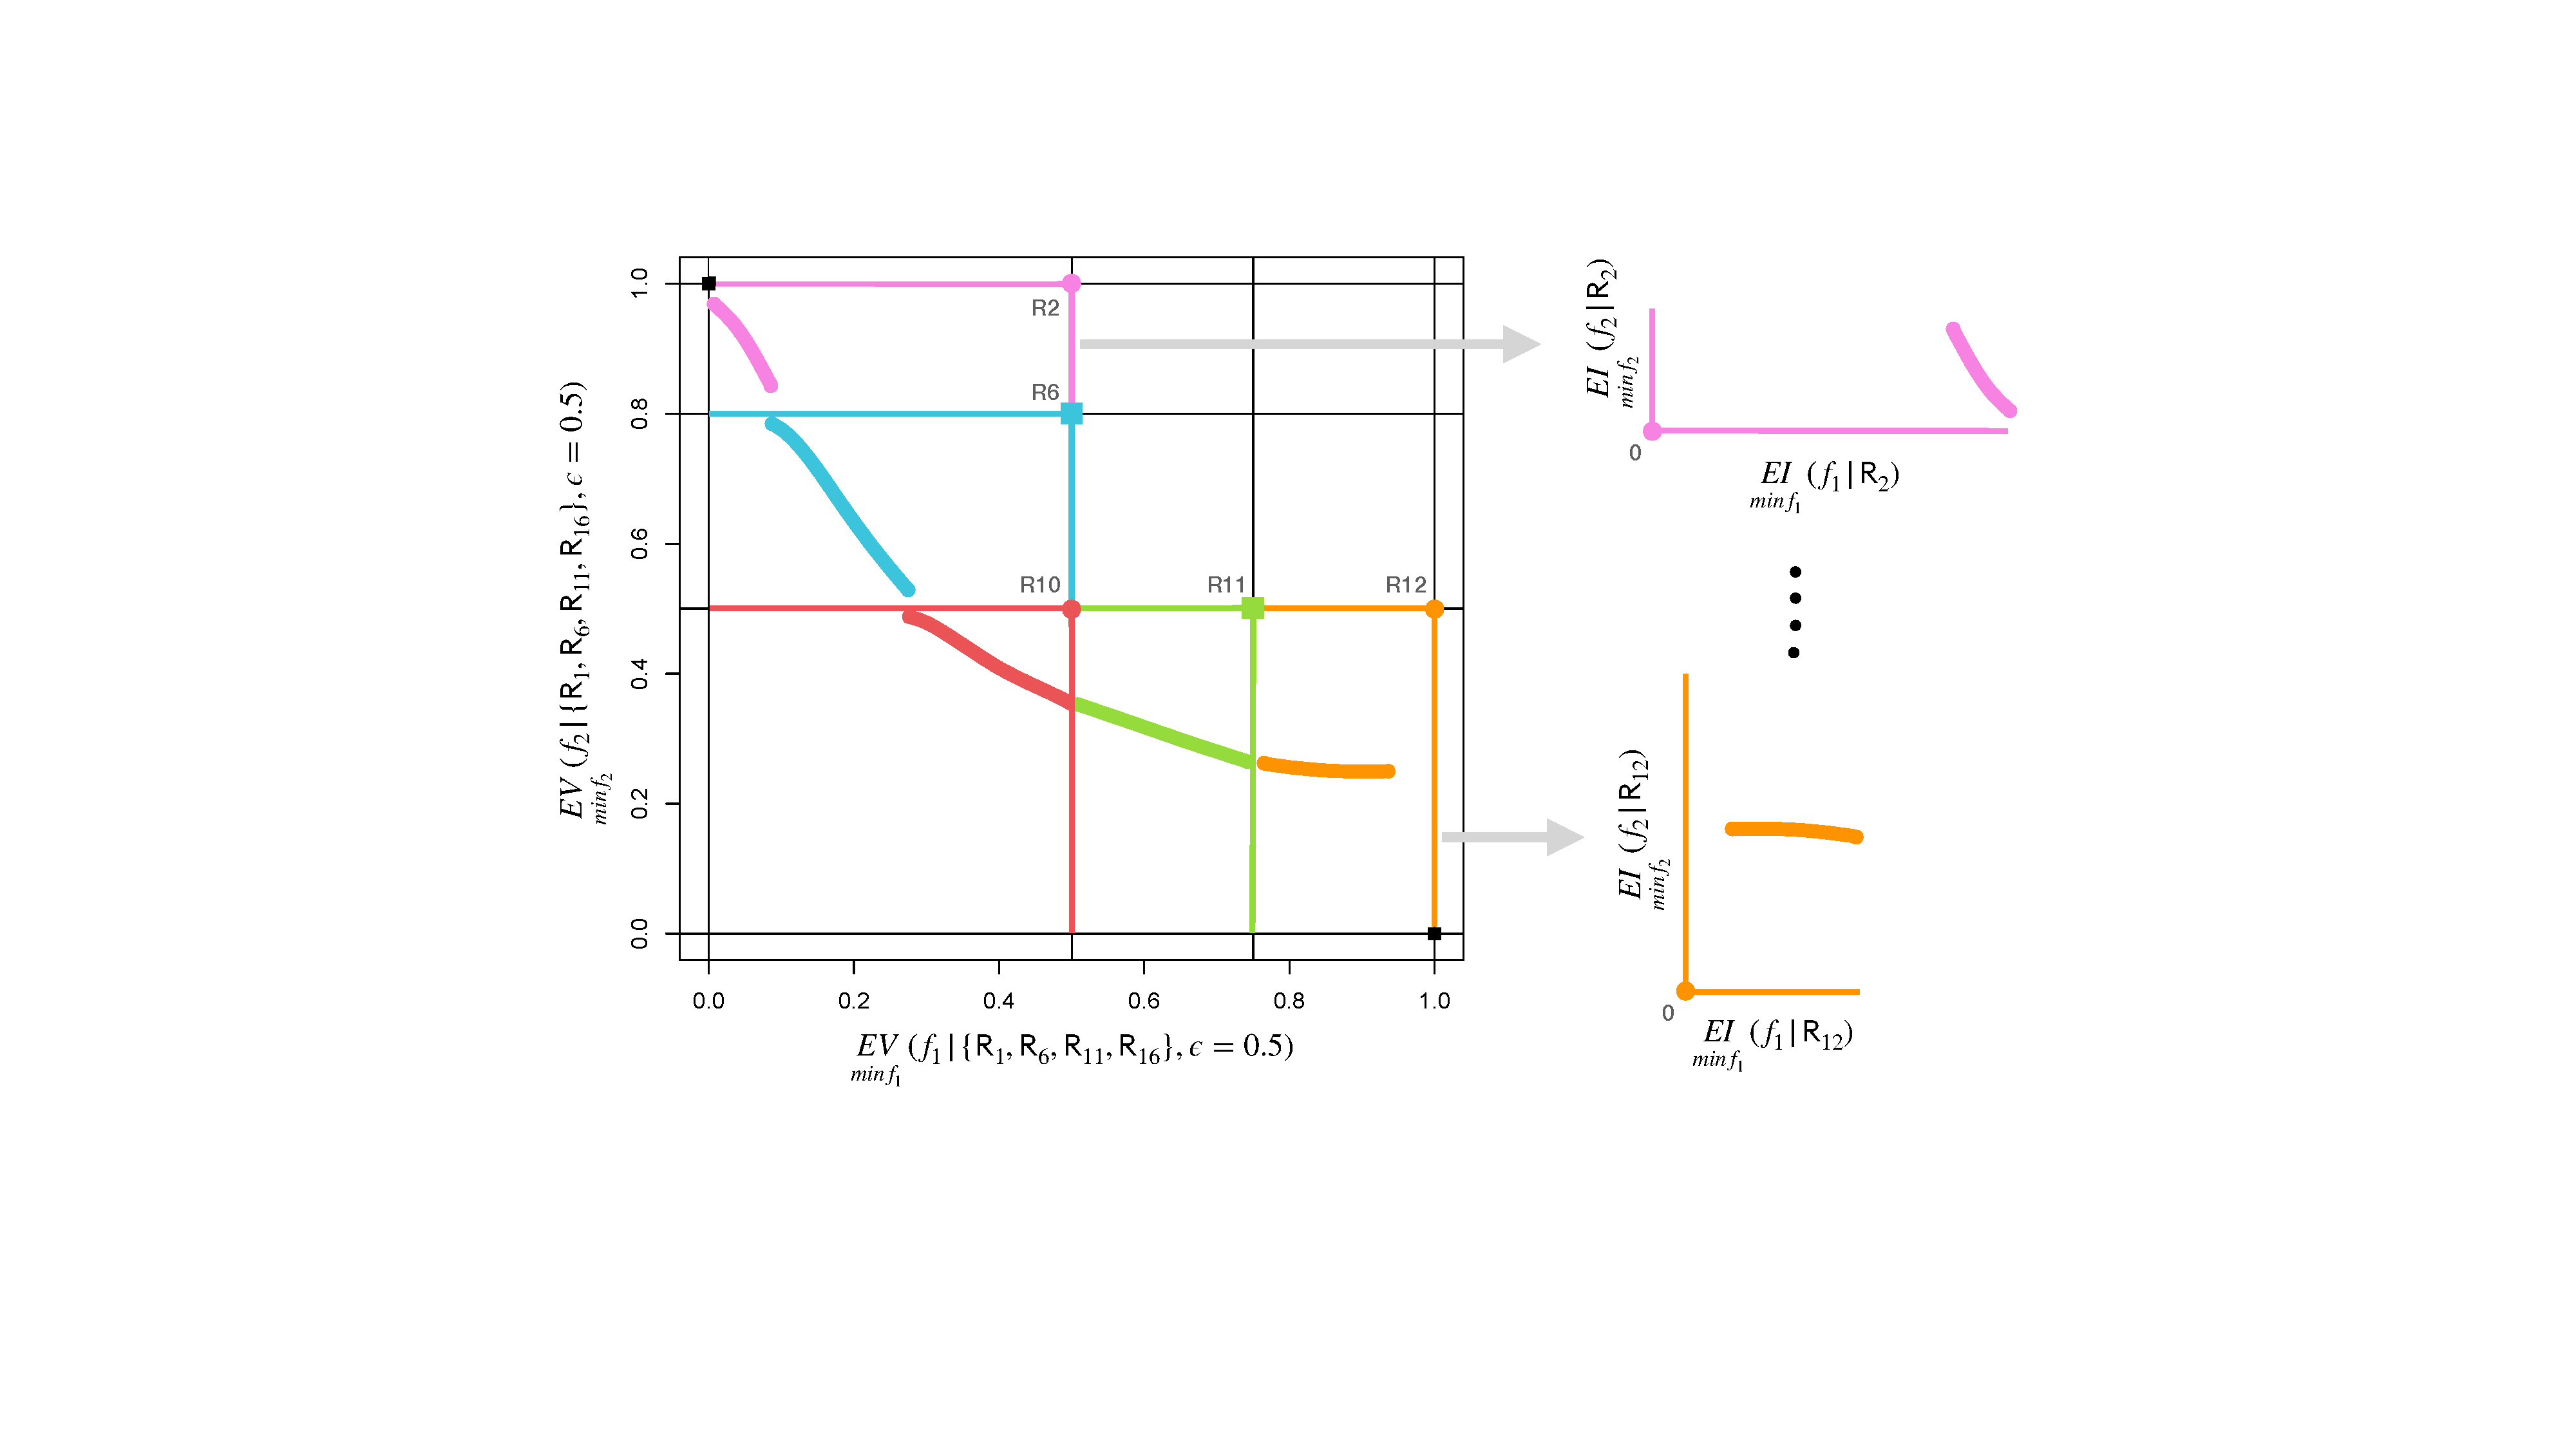
\includegraphics[scale=0.4]{Chapter5/Pictures/EV_rel_EI_ZDT1.pdf}
    \caption{Relation of $EV$ to reference point}
    \label{fig:EV_EIss}
 \end{figure}
 
 
 

Once $\mathscr{P}_{\hat{\mathcal{S}}}$ is obtained optimising Eq. \eqref{Optim_EVs} with NSGA-2, the problem leads to choosing the infill points among  $\mathscr{P}_{\hat{\mathcal{S}}}$. 
Firstly, we discuss the preference of choosing an improvement $\mathscr{I}_{\bm f^*} \in \mathfrak{I}_{\bm f^*}$, where the reference point ${\bm f^*}$ can be considered to define a part of $\bm f(\mathscr{P}_{\hat{\mathcal{S}}})$, i.e., $\{ \mathfrak{I}_{\bm f^*} \cap\bm f(\mathscr{P}_{\hat{\mathcal{S}}})\} \neq \emptyset$.
The part of the Pareto-front defined by ${\bm f^*}$ can hence be expressed as $\mathscr{P}_{\hat{\mathcal{S}}}^{\bm f^*} = \{ \mathfrak{I}_{\bm f^*} \cap \bm f(\mathscr{P}_{\hat{\mathcal{S}}})\}$, where the choice of an infill point in the set  $\mathfrak{I}_{\bm f^*}$ can be narrowed down to choosing a point  $\mathscr{I}_{\bm f^*} \in \bm f(\mathscr{P}_{\hat{\mathcal{S}}}^{\bm f^*})$. A suitable measure to quantify $\mathscr{I}_{\bm f^*}$ with respect to ${\bm f^*}$ can be given through hypervolume metric as

\begin{equation}\label{HVI_ref}
HVI(\mathscr{I}_{\bm f^*}|{\bm f^*})=\prod_{\mathsf{i}=1}^{\mathsf{m}} f_{\mathsf{i}}^*-\underset{min\,f_{\mathsf i}(\bm{x})}{EV}(\bm x|f^*_i)
\end{equation}

Hence, the most suitable choice of $\mathscr{I}_{\bm f^*} \in \bm f ( \mathscr{P}_{\hat{\mathcal{S}}}^{\bm f^*})$ is which maximises  $HVI(\mathscr{I}_{\bm f^*}|{\bm f^*})$, expressed as $\underset{\mathscr{I}_{\bm f^*} \in \bm f(\mathscr{P}_{\hat{\mathcal{S}}}^{\bm f^*})}{max} HVI(\mathscr{I}_{\bm f^*}|{\bm f^*})$.  It should be noted that, in this case, $HVI(\mathscr{I}_{\bm f^*}|{\bm f^*})$ is equivalent to ${EHVI}(\bm{x}|{\bm f^*})$, which is also similar to the criteria $mEI$ detailed in $\label{mEI}$, since $ f_{\mathsf{i}}^*-\underset{min\,f_{\mathsf i}(\bm{x})}{EV}(\bm x|f^*_i)=\underset{min\,f_{\mathsf i}(\bm{x})}{EI}(\bm x|f^*_i)$. The calculation of $HVI$ in this case is analytical and simple irrespective of the dimensions.\\

The choice of $\underset{\mathscr{I}_{\bm f^*} \in \bm f(\mathscr{P}_{\hat{\mathcal{S}}}^{\bm f^*})}{max} HVI(\mathscr{I}_{\bm f^*}|{\bm f^*})$ essentially expresses the best $HVI$ with respect to $\bm f^*$, but it makes no relation of $HVI$ relative to $\bm f(\mathscr{P}_{\mathcal S})$. 
While $HVI$ relative to $\bm f(\mathscr{P}_{\mathcal S})$ can simply be expressed as ${HVI}(\mathscr{I} |\bm f(\mathscr{P}_{\mathcal{S}}), \bm{\mathsf{R}})$\footnote{$\mathscr{I}$ is an arbitrary improvement point where we do not focus on the reference point with which it is defined, contrary to $\mathscr{I}_{\bm f^*}$}, this is quite an expensive strategy to pick an infill point from $\mathscr{P}_{\hat{\mathcal{S}}}$, since this requires evaluation of ${HVI}(\mathscr{I} |\bm f(\mathscr{P}_{\mathcal{S}}), \bm{\mathsf{R}})$ for all $\mathscr{I} \in  \mathscr{P}_{\hat{\mathcal{S}}}$. Since $HVI$ with respect to $\bm f^*$ is known, it can be said that the relation of $\mathscr{I}_{\bm f^*}$  with respect to $\mathscr{P}_{\hat{\mathcal{S}}}$ can be defined by counting the ${HVI}({\bm f^*} |\bm f(\mathscr{P}_{\mathcal{S}}), \bm{\mathsf{R}})$, expressed as

\begin{equation}
HVI_{\uplus}(\mathscr{I}_{\bm f^*}|\bm f(\mathscr{P}_{\mathcal{S}}), \bm{\mathsf{R}})=HVI(\mathscr{I}_{\bm f^*}|{\bm f^*})+
{HVI}({\bm f^*} |\bm f(\mathscr{P}_{\mathcal{S}}), \bm{\mathsf{R}})
\end{equation} 

The idea is that instead of defining ${HVI}(\mathscr{I} |\bm f(\mathscr{P}_{\mathcal{S}}), \bm{\mathsf{R}})$ for all $\mathscr{I} \in  \mathscr{P}_{\hat{\mathcal{S}}}$, the computation of  higher complexity $HVI((.)|\bm f(\mathscr{P}_{\mathcal{S}}), \bm{\mathsf{R}})$ is limited to the reference points $\bm g_o \in \mathscr{G}$ for which $\{ \mathfrak{I}_{\bm g_o} \cap \mathscr{P}_{\hat{\mathcal{S}}}\} \neq \emptyset$. With the definition of $HVI((.)|\bm f(\mathscr{P}_{\mathcal{S}}), \bm{\mathsf{R}})$ for a $\bm g_o$, the definition of $HVI$ for any improvement  
$\mathscr{I}_{\bm f^*} \in \mathfrak{I}_{\bm f^*}$ is given by simple product relation in \eqref{HVI_ref}. The infill point from ${\mathscr P}_{\hat{\mathcal S}}$ to define the maximum $HVI$ relative to $\mathscr P_{\mathcal S}$ can be expressed as

\begin{equation}
\bm x^{\iota}= \underset{\bm x \in \mathcal{X}}{arg\, max} \Big\{ HVI_{\uplus}(\mathscr{I}_{\bm g_o}(\bm x)|\bm f(\mathscr{P}_{\mathcal{S}}),\bm{\mathsf{R}})|  \{\mathfrak{I}_{\bm g_o}\cap \bm f(\mathscr{P}_{\hat{\mathcal S}})\} \neq \emptyset, \forall \bm g_o \in\mathscr{G},\forall \bm x \in \mathcal{X} \Big\}
\end{equation} 

Essentially, we scalarise $\mathscr{I} \in \mathscr{P}_{\hat{\mathcal S}}$ to find a single infill point $\bm x^{\iota}$. But this necessarily does not have to be the case, since we have the optimal measure of $\mathscr{I}$ in multiobjective context as $\mathscr{P}_{\hat{\mathcal S}}$, this gives way to lot of possibilities of choosing infill points from $\mathscr{P}_{\hat{\mathcal S}}$, considering simultaneous improvement in hypervolume with batch-selection and enhancing diversity.
 We do not yet focus on defining batch-selection in this thesis, exploiting the property of $\mathscr{G}$.\\


%The preference of choosing an improvement $\mathscr{I}_{\bm f^*} \in \mathfrak{I}_{\bm f^*}$ with respect to its reference point ${\bm f^*}$ through $\underset{\mathscr{I}_{\bm f^*} \in \mathscr{P}_{\hat{\mathcal{S}}}^{\bm f^*}}{max} HVI(\mathscr{I}_{\bm f^*}|{\bm f^*})$ can be interpreted as optimising for local definition of improvement with respect to its reference point. This is especially more true when the reference point defines improvements which contribute to $\mathscr{P}_{\hat{\mathcal{S}}}$. But this brings the question of choosing a reference point ${\bm f^*}$ to choose $\mathscr{I}_{\bm f^*}$, where this process can be interpreted as optimising for global definition of improvement. The most easiest is to quantify the reference points defining $\mathscr{P}_{\hat{\mathcal{S}}}$ through Pareto-front ranking. This means that any reference point(s) which has better rank define better improvements with respect to that reference point globally. Meanwhile if a set of reference points belong to a same rank, then preference can be inclined to the reference point which  has the maximum  $HVI$. Even though $HVI$ is defined independently with respect to a particular reference point, comparisons can be plausible since the reference points belong to the same rank. Hence, the choice of reference value through Pareto-front ranking naturally leads to global optimisation to choose the best set $\mathfrak{I}$ from which local optimisation of $\mathscr{I}$ can be defined.\\

\\

We focus on the approach of clustering improvements in $\mathscr{P}_{\hat{\mathcal{S}}}$ through $K$-means and a point can be sampled from each cluster to enhance diversity, which also defines the possibility of parallelization. 
Considering simplicity, we chose the most uncertain point in each cluster, given by the uncertainty of the $\mathcal{GP}$ models. Hence, this strategy tries to reduce uncertainty on the $\mathcal{GP}$ meta-models for the points in $\mathscr{P}_{\hat{\mathcal{S}}}$, rather than to seek improvement through quality indicators. But care should be taken, since adjacent points between adjacent clusters can have the same measure of uncertainty and hence can lead to samples for parallelization from the same part of the design space.\\

We show the effect of $\epsilon$ through the following plots, where the idea is to show the behaviour for a range of predictions. The range is defined for  $\hat{\mu} {(\bm x)} \in [50,200]$, distinguished with color scale and $\hat{\sigma} {(\bm x)} \in [5,50]$ defined on the vertical axis. The horizontal axis defines the $EV$ criteria with four possible reference values $\{ 62.5,75,100,150\}$ to choose for any prediction. Firstly, to have a general idea, we give the plot of $\hat{\mu} {(\bm x)}$ against $\hat{\sigma} {(\bm x)}$

\begin{figure}[h!]
    \centering
    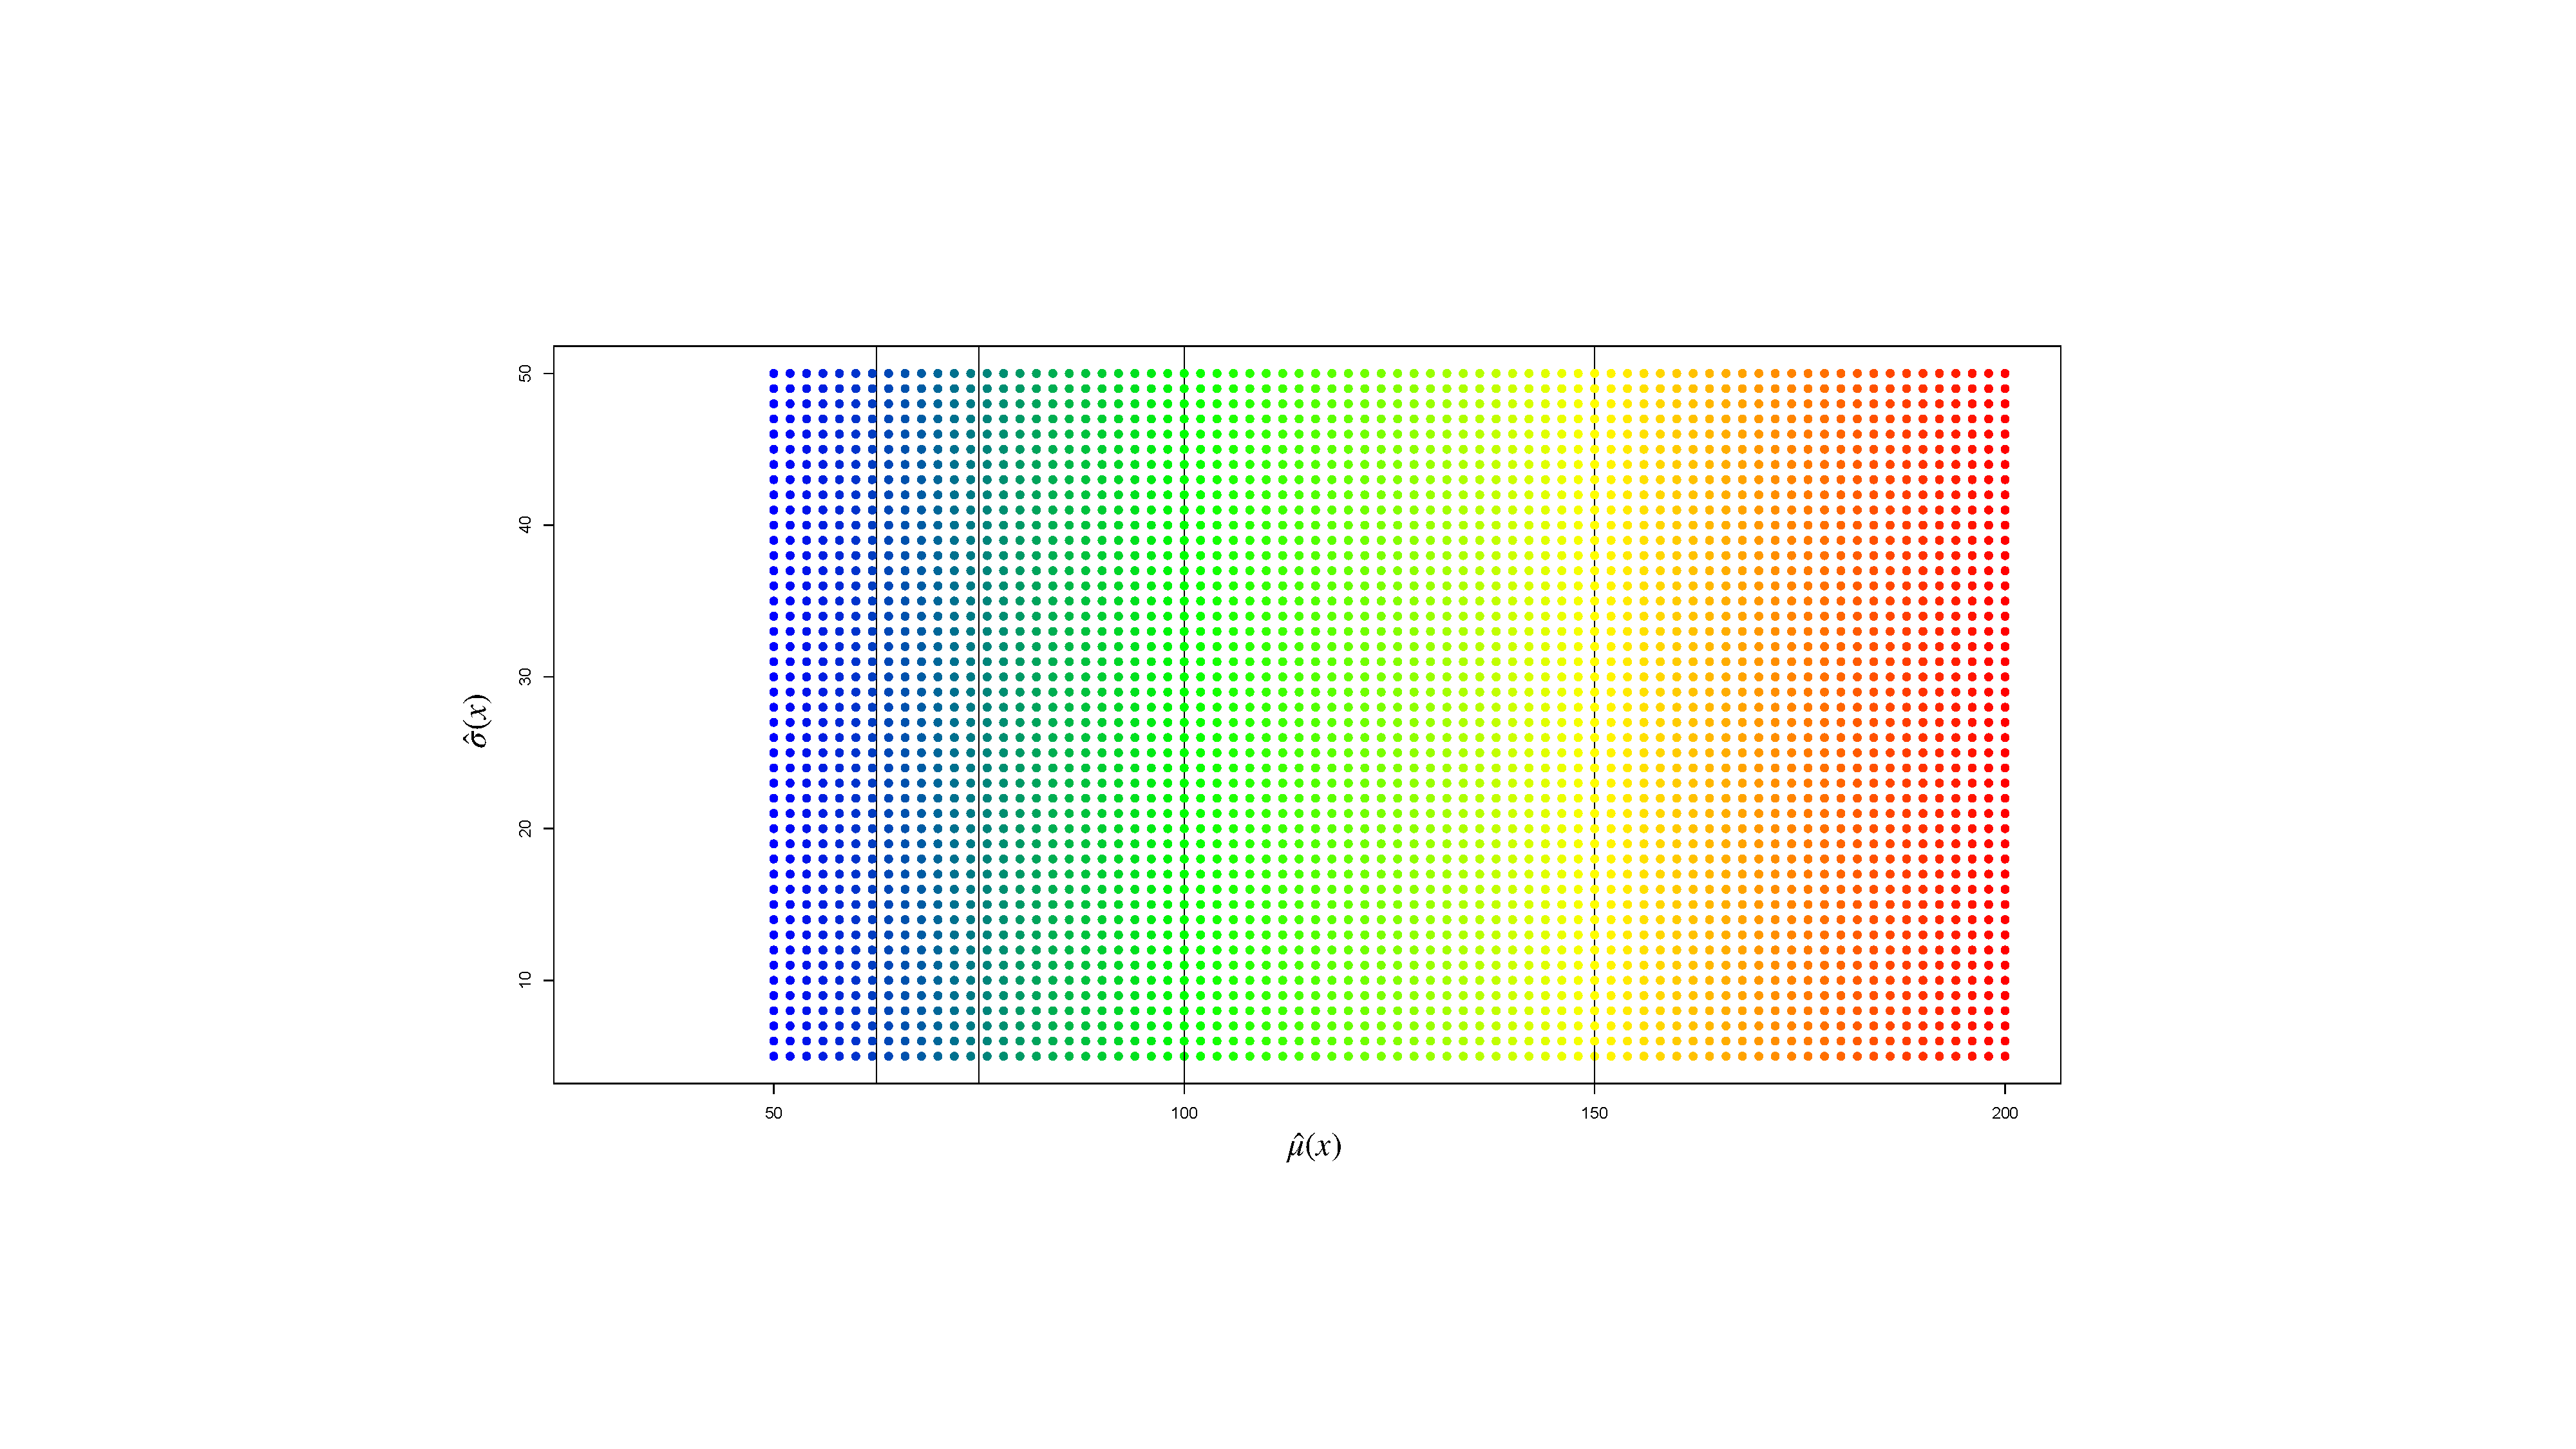
\includegraphics[scale=0.3]{Chapter5/Pictures/EV_mean}
    \caption{Plot showing the characteristics of choosing }
    \label{fig:EV_1.5}
\end{figure}





\begin{figure}[h!]
    \centering
    \subfloat[$\epsilon=0$]{
    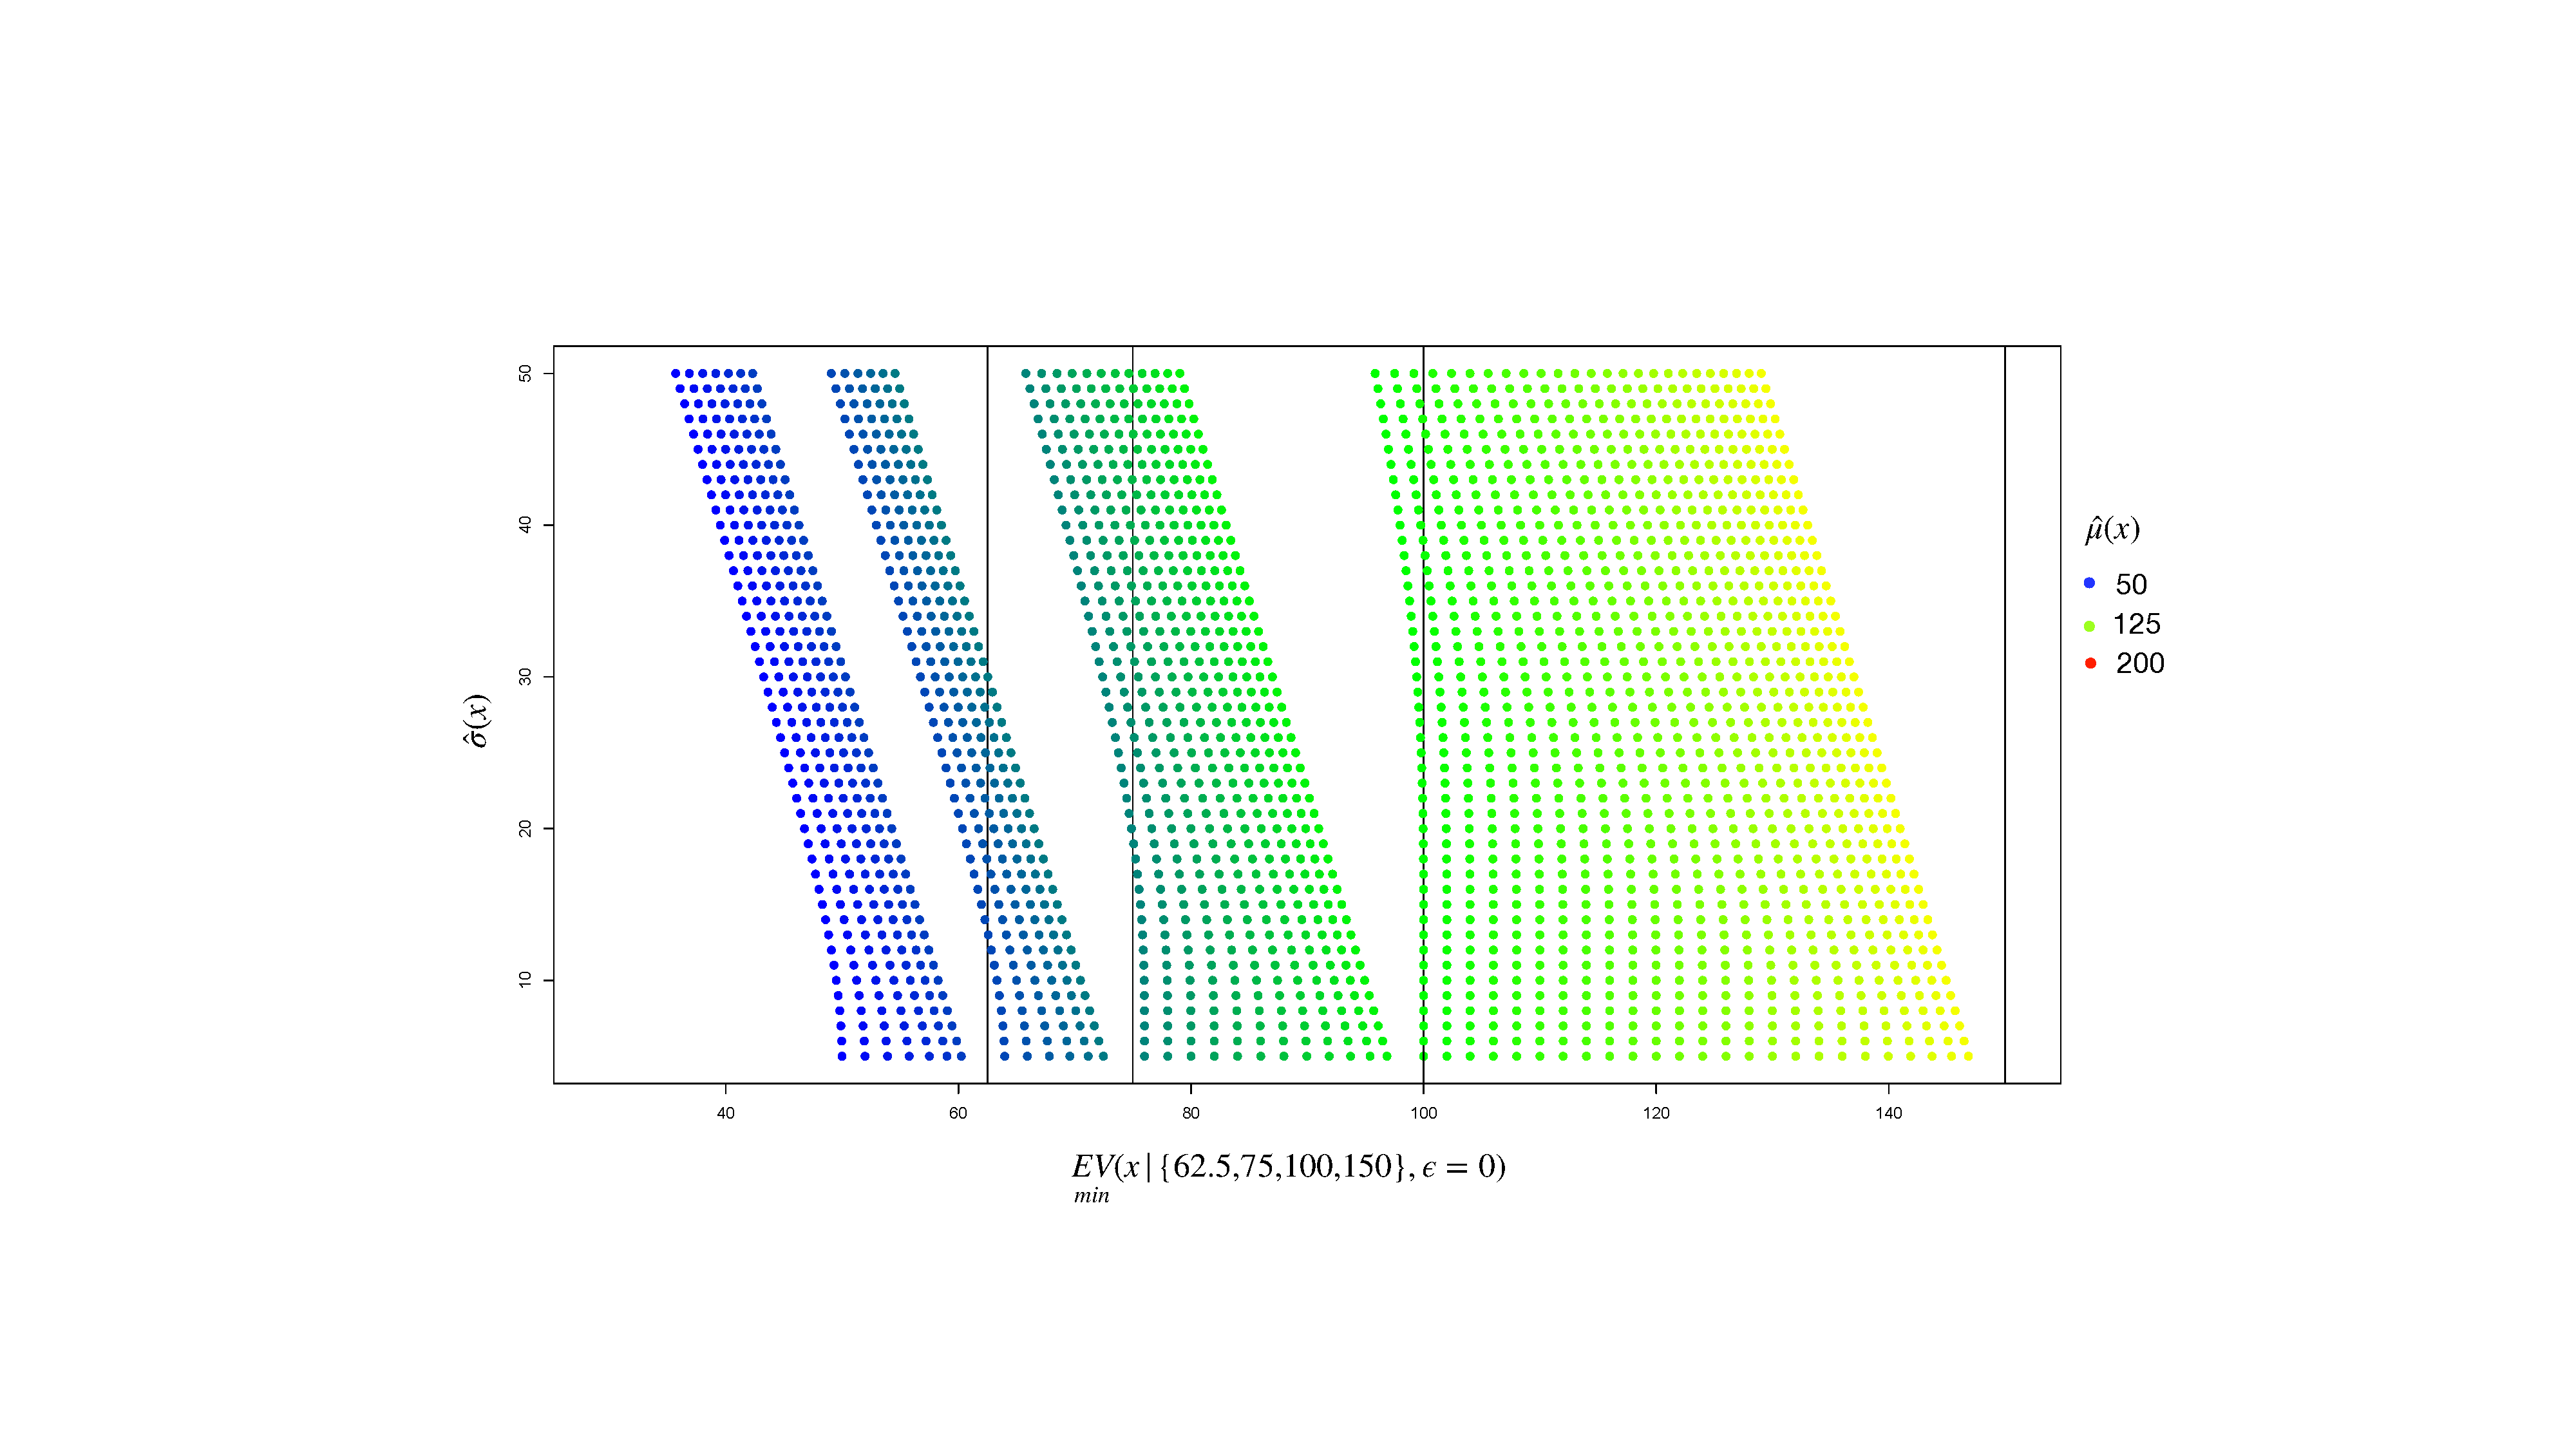
\includegraphics[scale=0.3]{Chapter5/Pictures/EV_0}}\\
    \subfloat[$\epsilon=0.5$]{
    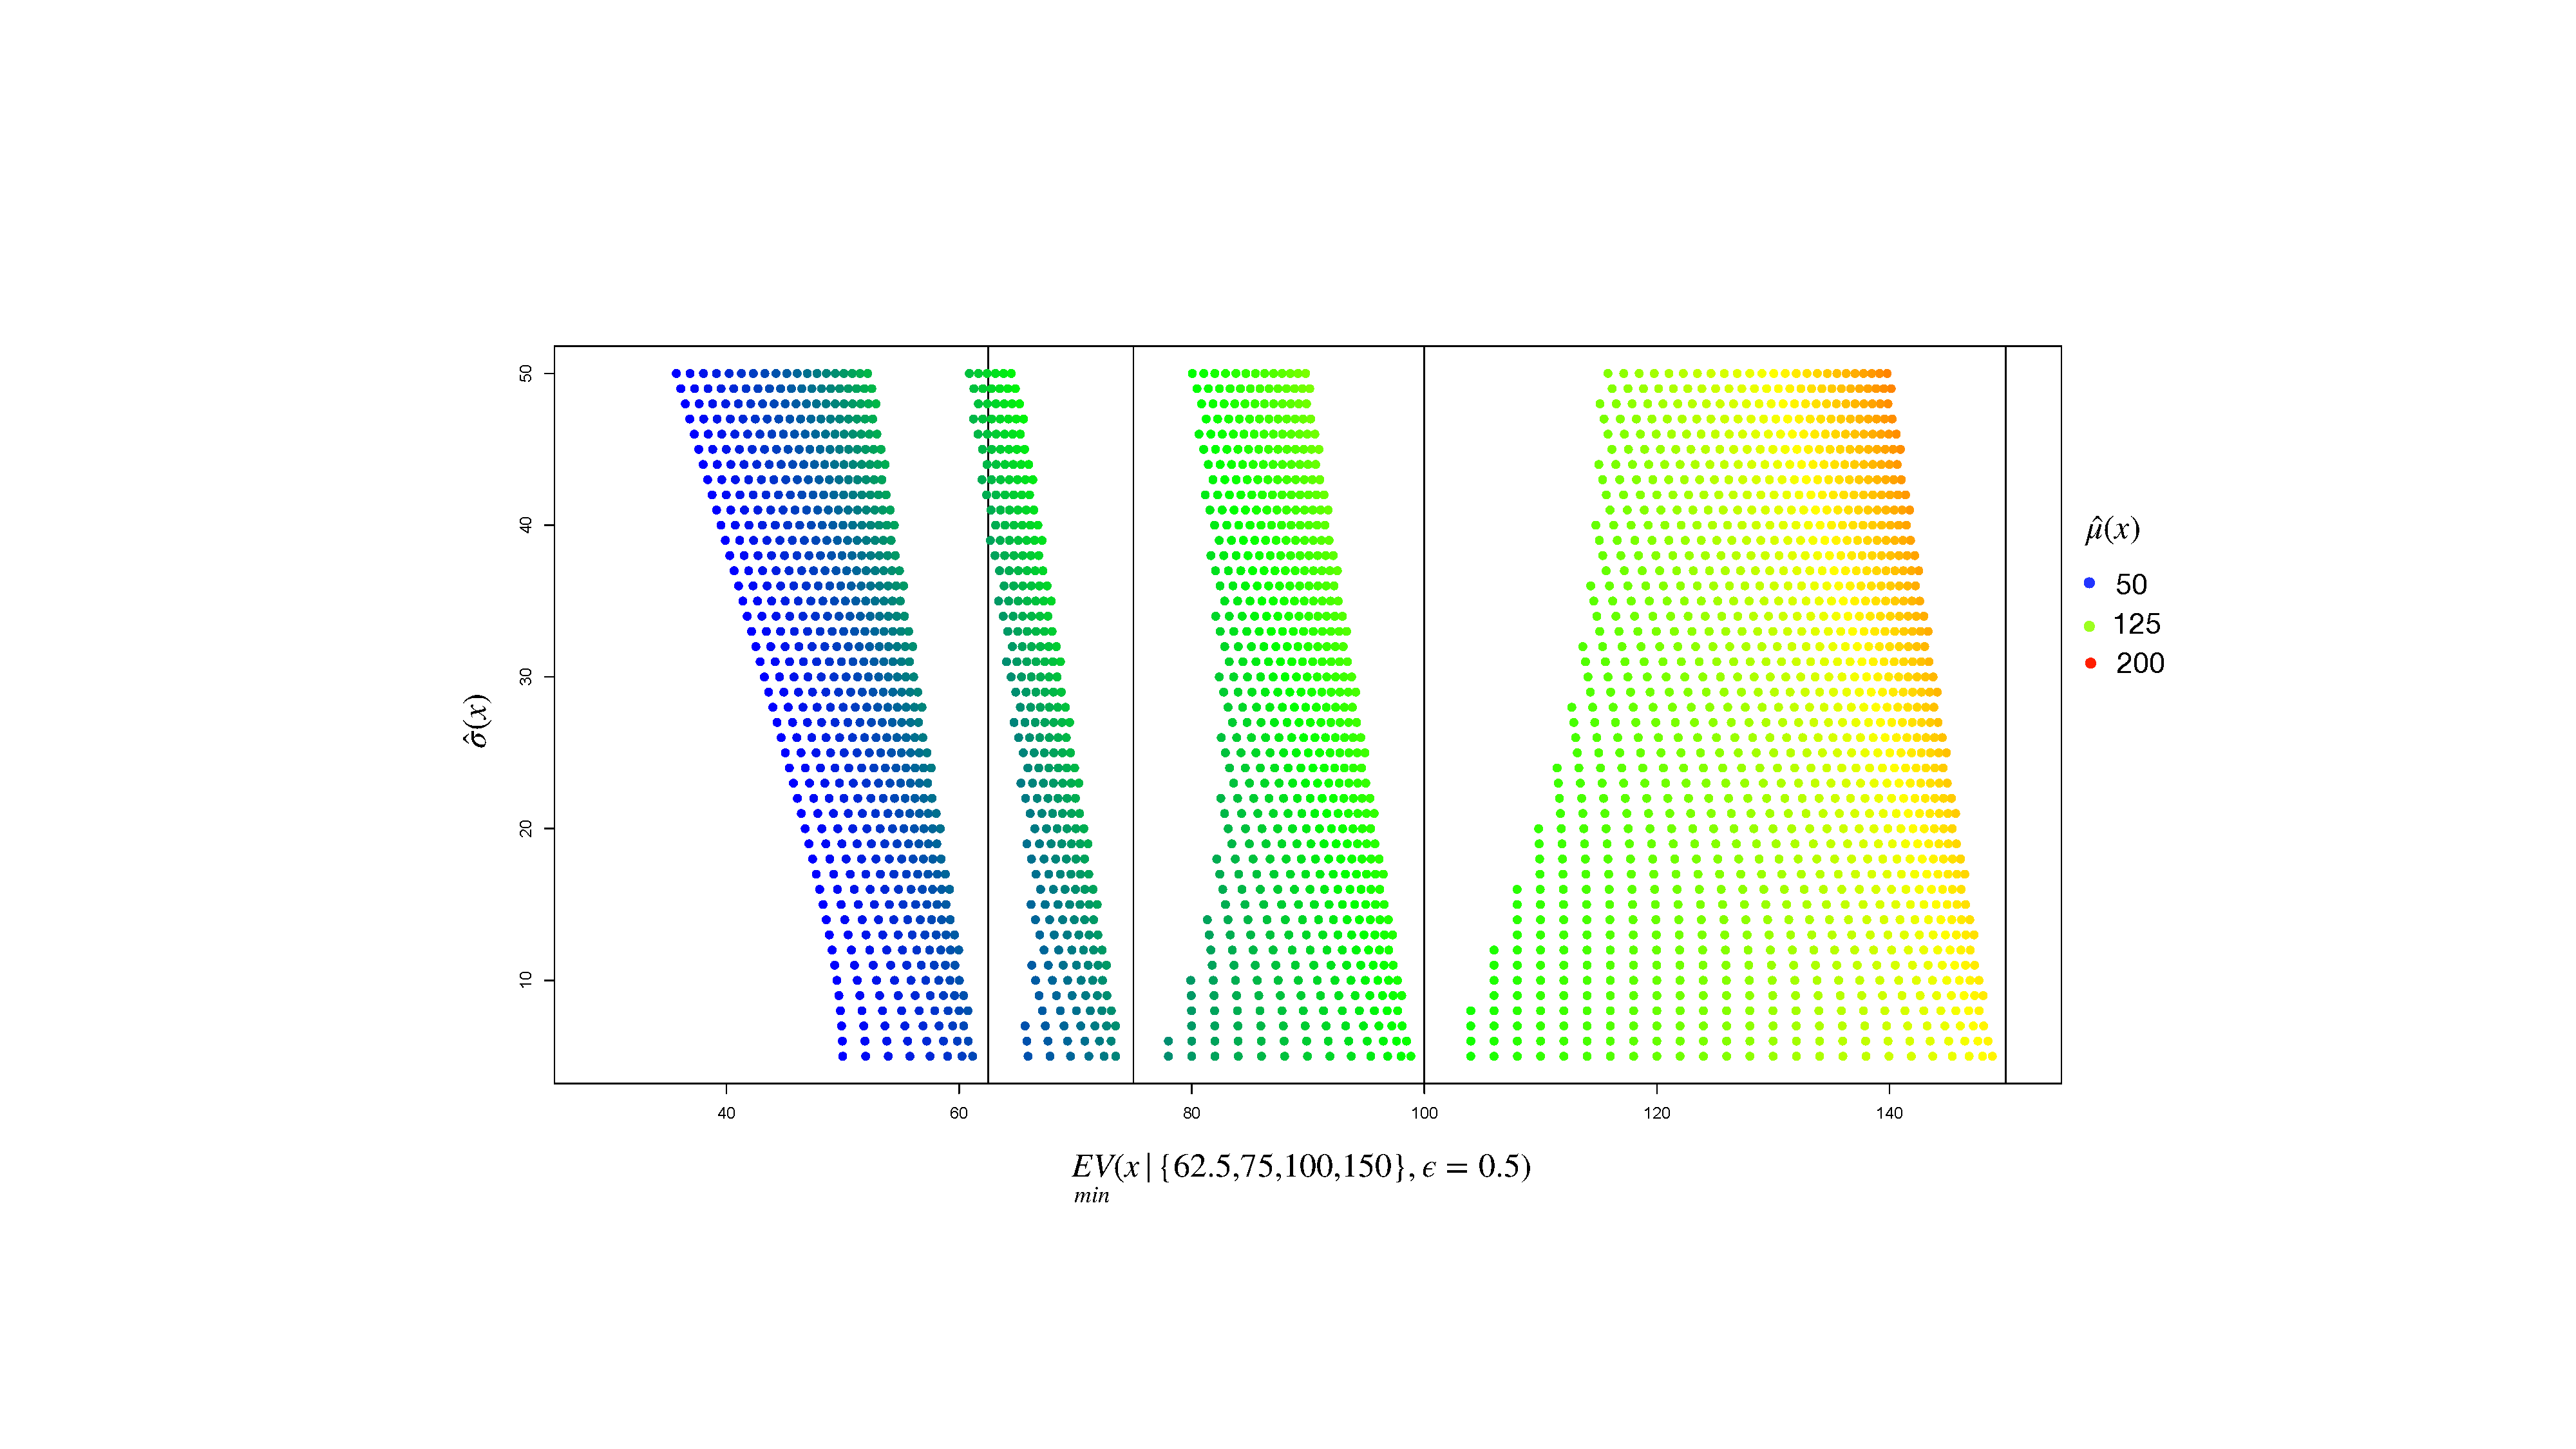
\includegraphics[scale=0.3]{Chapter5/Pictures/EV_05}}
    \end{figure}
\clearpage
    
   \begin{figure}[h!]
    \centering 
    \subfloat[$\epsilon=1$]{
    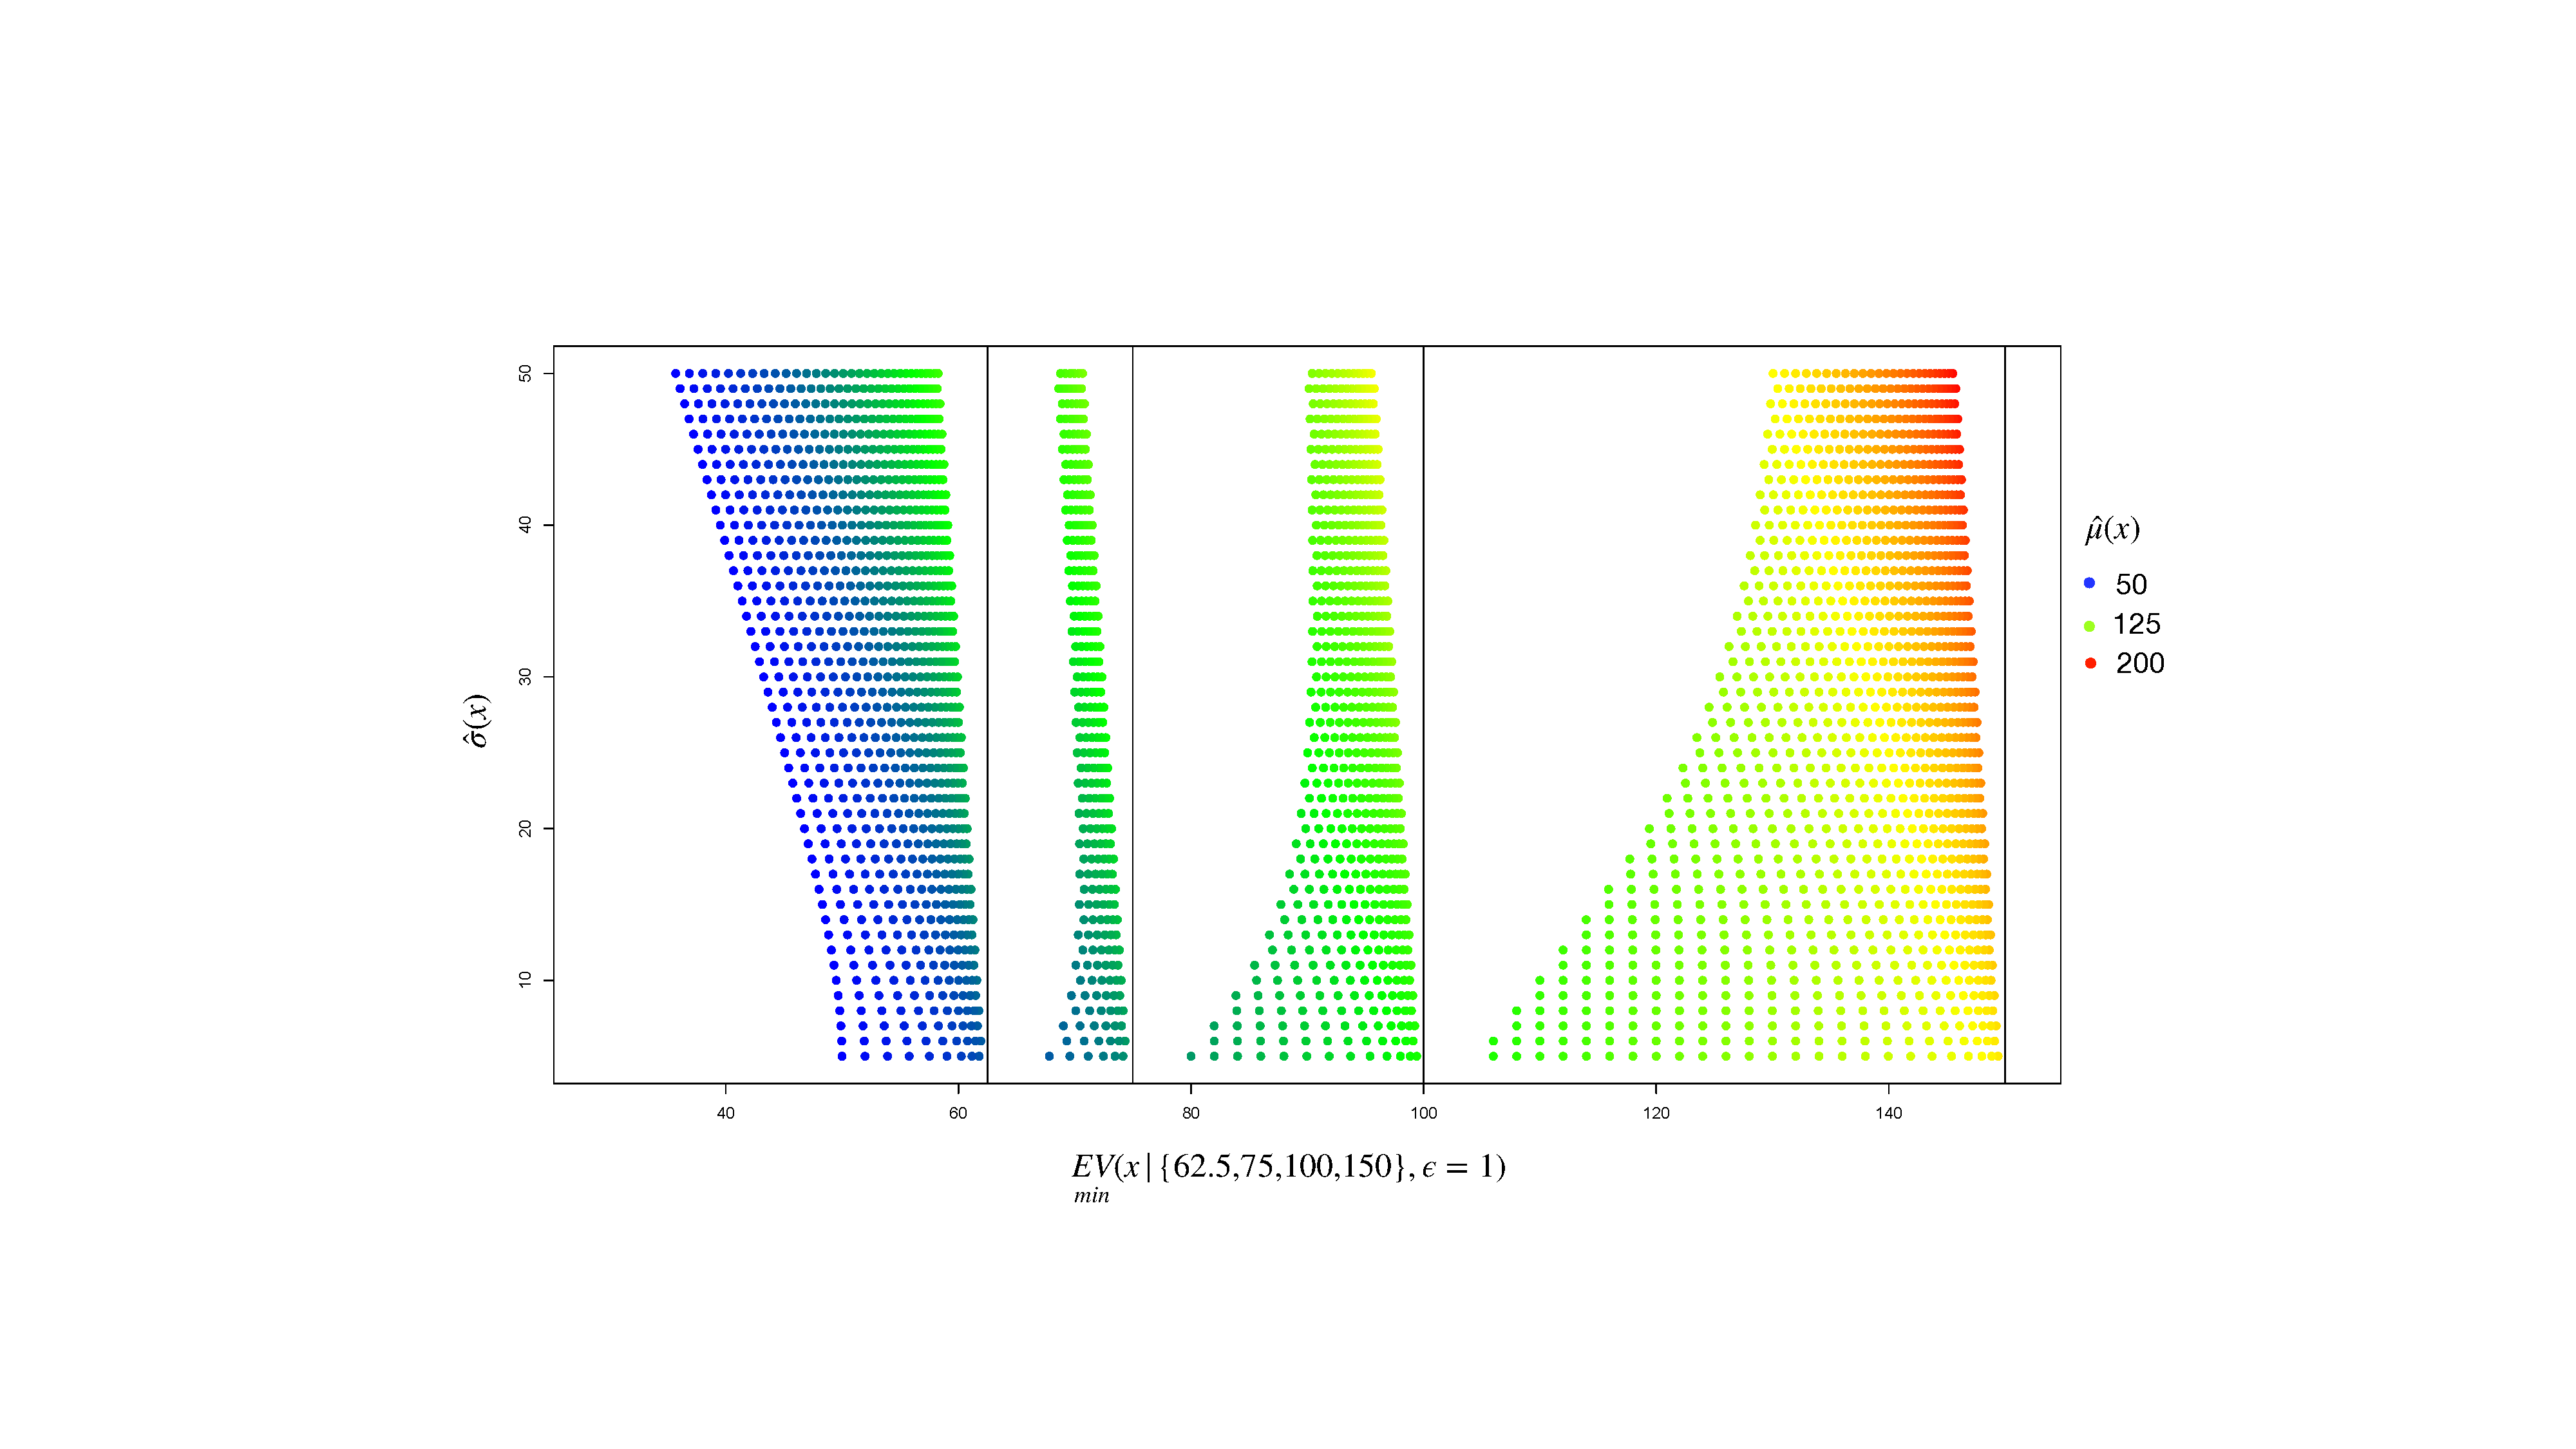
\includegraphics[scale=0.3]{Chapter5/Pictures/EV_1}}\\
    \subfloat[$\epsilon=1.5$]{
    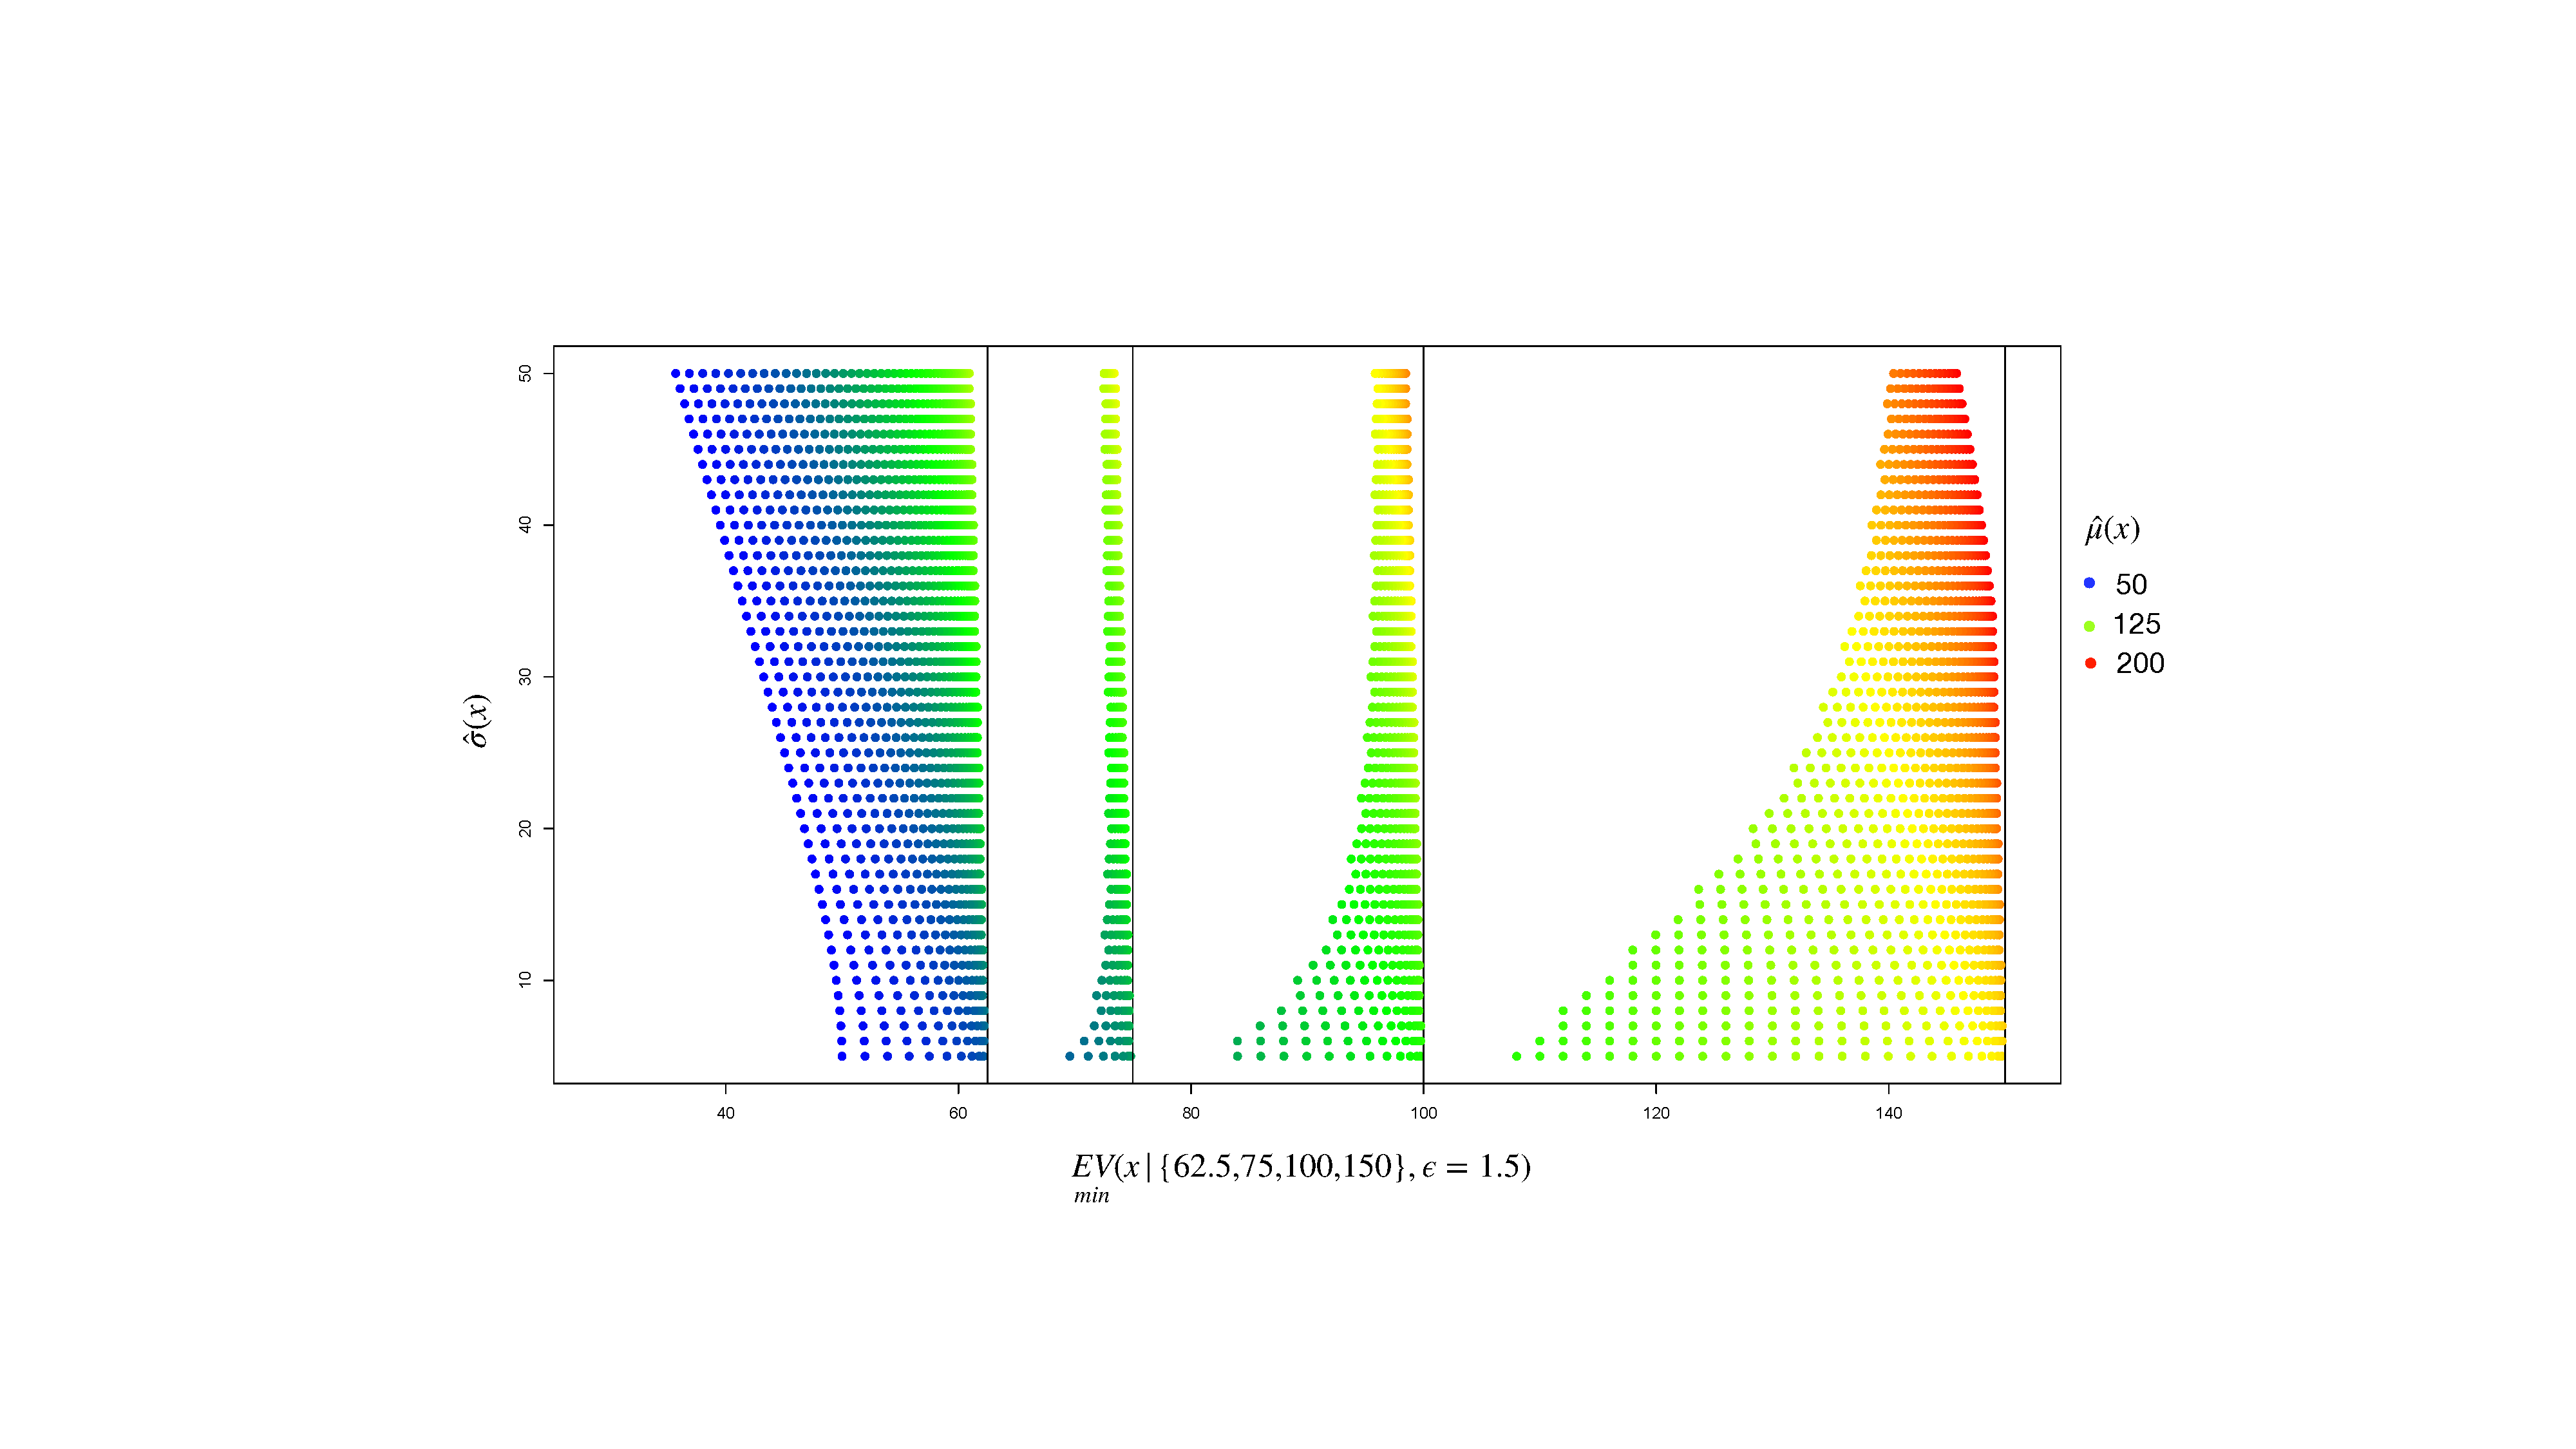
\includegraphics[scale=0.3]{Chapter5/Pictures/EV_15}}
\end{figure}

Some of the special cases where it converges to the cases of Nadir to Utopian value of reference is shown below

\begin{figure}[h!]
    \centering
    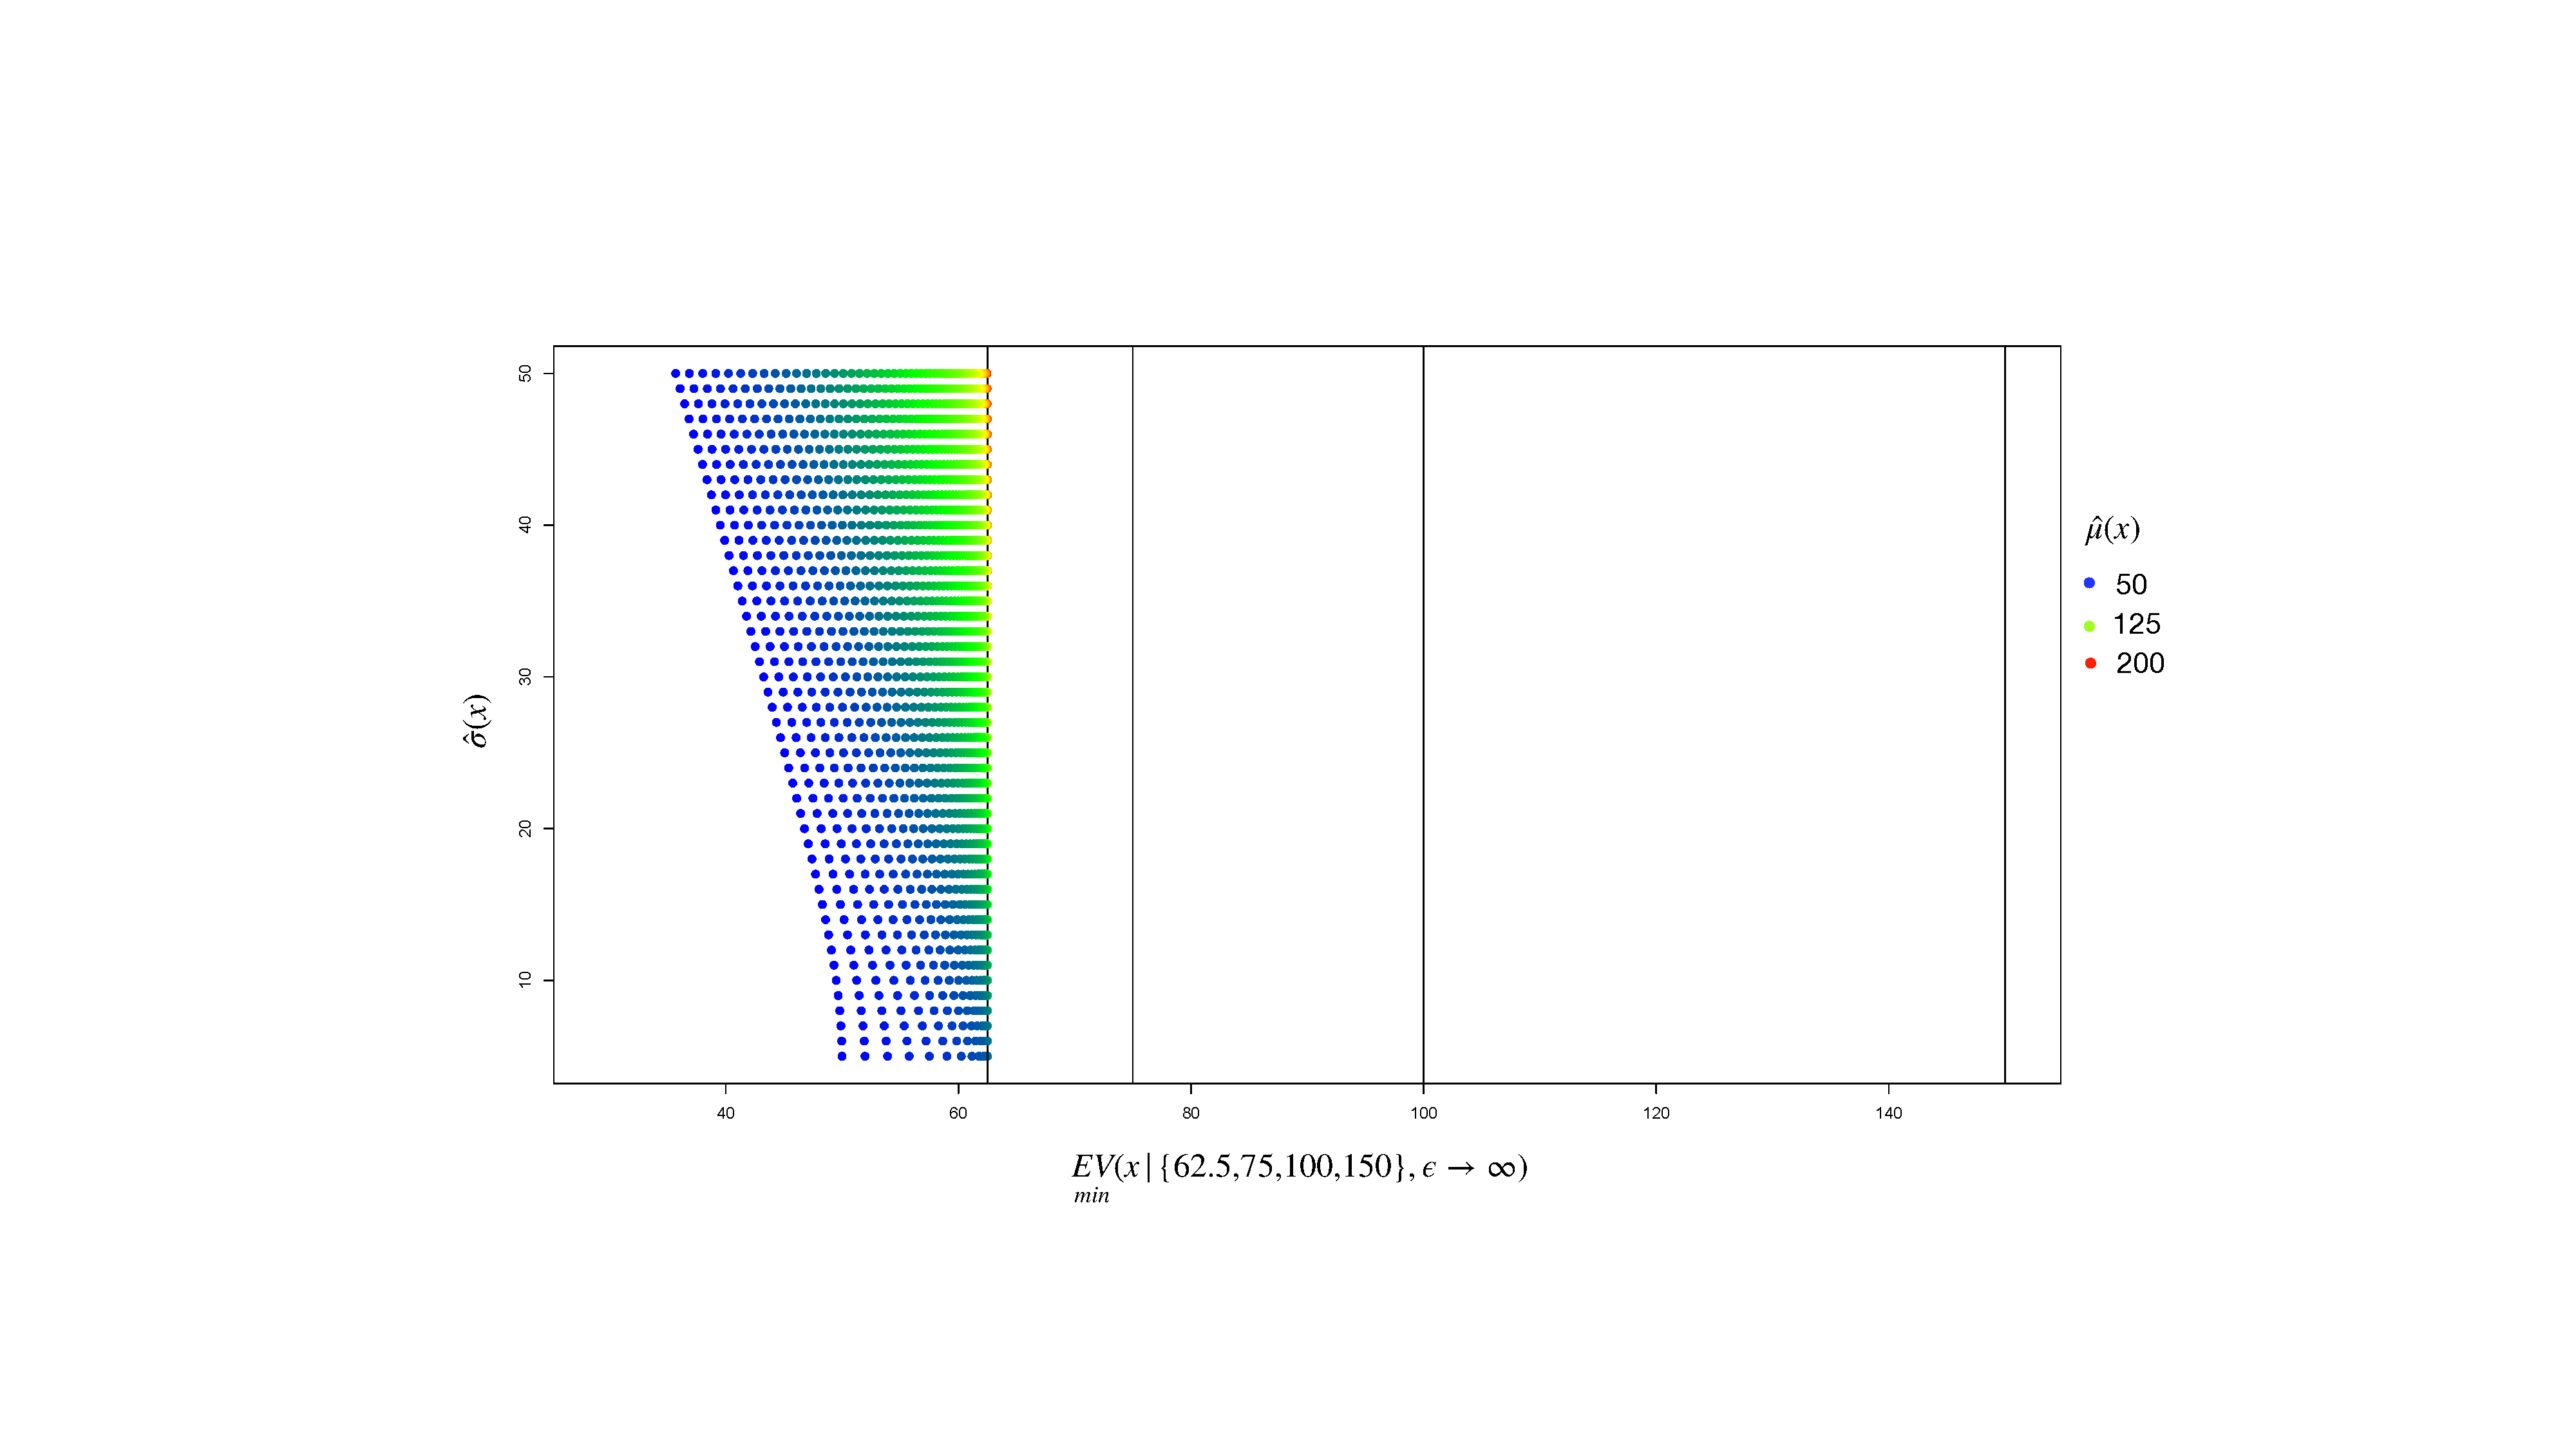
\includegraphics[scale=0.3]{Chapter5/Pictures/EV_inf}
    \caption{ $\epsilon \rightarrow \infty$}
    \label{fig:EV_1.5}
\end{figure}

\begin{figure}[h!]
    \centering
    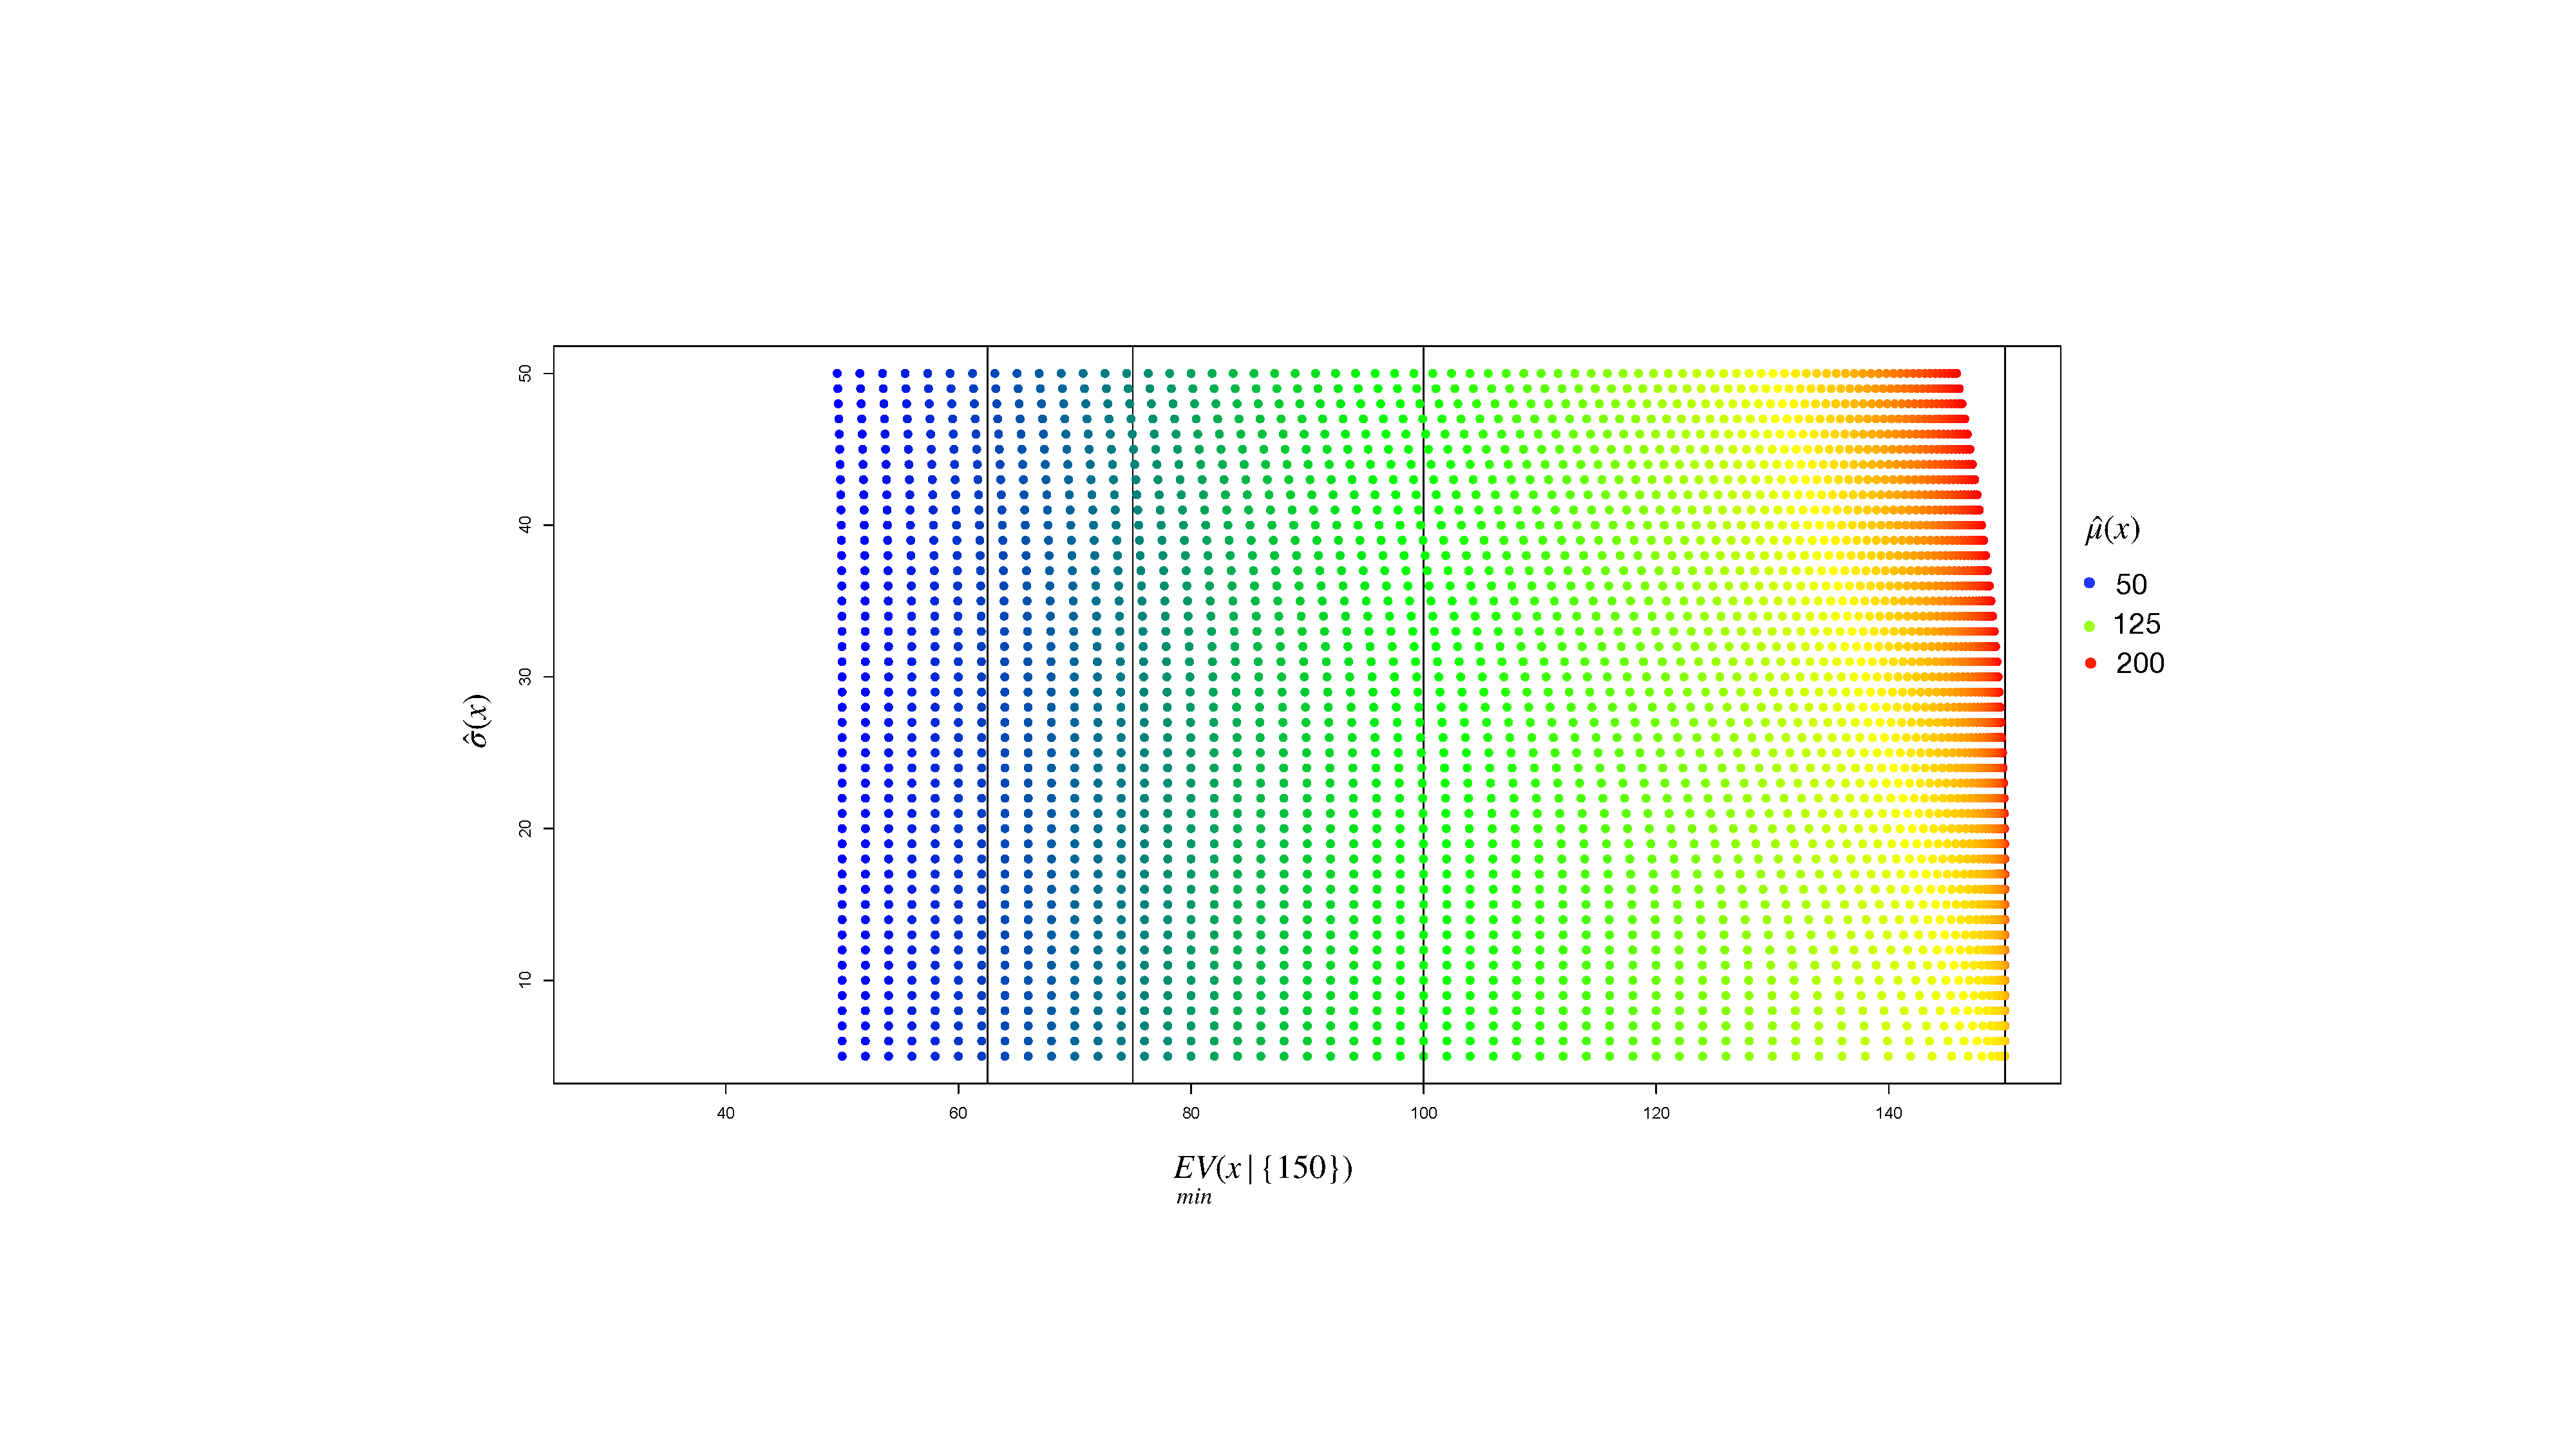
\includegraphics[scale=0.3]{Chapter5/Pictures/EV_nad}
    \caption{EV with Nadir value as reference}
    \label{fig:EV_1.5}
\end{figure}










